% Anonymous submission source (UniReps 2026 workshop at NeurIPS 2026).
% Style: the official neurips_2026.sty must be placed in this directory for submission (build.sh official).
% build.sh proxy uses a community copy of the 2026 style only to approximate layout; build.sh fallback uses a
% plain-article stand-in. Every number in the text is a macro generated from raw results.
\documentclass{article}
\IfFileExists{neurips_2026.sty}{%
  \usepackage[dblblindworkshop]{neurips_2026}%
  \workshoptitle{UniReps: Unifying Representations in Neural Models}%
}{%
  \usepackage[letterpaper,textwidth=5.5in,textheight=9in,top=1in,headheight=12pt,headsep=25pt,footskip=30pt]{geometry}%
  \usepackage[numbers,sort&compress]{natbib}%
  \usepackage{mathptmx}%
}
\usepackage[utf8]{inputenc}
\usepackage[T1]{fontenc}
\usepackage{amsmath,amssymb,amsthm}
\usepackage{booktabs}
\usepackage{graphicx}
\usepackage{xcolor}
\usepackage[hidelinks,pdfusetitle=false]{hyperref}
\hypersetup{pdfauthor={},pdftitle={Closing the Algebra Is Not Enough},pdfsubject={},pdfkeywords={},pdfcreator={},pdfproducer={}}
\usepackage{microtype}
\renewcommand{\ttdefault}{pcr}
\emergencystretch=2em
\makeatletter\newcommand{\tabinput}[1]{\@@input #1 }\makeatother
\graphicspath{{../../figures/final/}{../../figures/review/}}
% AUTO-GENERATED by scripts/analyze_final.py from raw run files. Do not edit.
\newcommand{\NSteps}{4000}
\newcommand{\NLambda}{3}
\newcommand{\NNseeds}{20}
\newcommand{\NNpairs}{10}
\newcommand{\NNabl}{10}
\newcommand{\NSOtwoBNrefClosure}{0.000}
\newcommand{\NSOtwoBNrefClosureSd}{0.000}
\newcommand{\NSOtwoBNrefGtdistance}{9.1\times10^{-5}}
\newcommand{\NSOtwoBNrefGtdistanceSd}{8.8\times10^{-5}}
\newcommand{\NSOtwoBNrefMseonestep}{0.0026}
\newcommand{\NSOtwoBNrefMseonestepSd}{0.0010}
\newcommand{\NSOtwoBNrefMseonezerostep}{0.0063}
\newcommand{\NSOtwoBNrefMseonezerostepSd}{0.0027}
\newcommand{\NSOtwoBNrefCompositionmse}{3.9\times10^{-4}}
\newcommand{\NSOtwoBNrefCompositionmseSd}{7.8\times10^{-5}}
\newcommand{\NSOtwoBNrefActiontruth}{0.039}
\newcommand{\NSOtwoBNrefActiontruthSd}{0.006}
\newcommand{\NSOtwoBNrefCkatruth}{0.981}
\newcommand{\NSOtwoBNrefCkatruthSd}{0.003}
\newcommand{\NSOtwoBNrefParticipationratio}{2.00}
\newcommand{\NSOtwoBNrefParticipationratioSd}{0.00}
\newcommand{\NSOtwoBNrefCommutatornorm}{0.000}
\newcommand{\NSOtwoBNrefCommutatornormSd}{0.000}
\newcommand{\NSOtwoBNrefRuntimes}{44.5}
\newcommand{\NSOtwoBNrefRuntimesSd}{2.0}
\newcommand{\NSOtwoBNrefGramcondition}{1.00}
\newcommand{\NSOtwoBNrefGramconditionSd}{0.00}
\newcommand{\NSOtwoBNrefClosurewhitened}{0.000}
\newcommand{\NSOtwoBNrefClosurewhitenedSd}{0.000}
\newcommand{\NSOtwoBNrefCatCorrectclosed}{20}
\newcommand{\NSOtwoBNrefCatIncorrectclosed}{0}
\newcommand{\NSOtwoBNrefCatNonclosed}{0}
\newcommand{\NSOtwoBNrefCatCollapsed}{0}
\newcommand{\NSOtwoBNrefChiral}{0}
\newcommand{\NSOtwoBNrefBadaction}{0}
\newcommand{\NSOtwoBNrefCcrateLo}{84}
\newcommand{\NSOtwoBNrefCcrateHi}{100}
\newcommand{\NSOtwoBNClosure}{0.000}
\newcommand{\NSOtwoBNClosureSd}{0.000}
\newcommand{\NSOtwoBNGtdistance}{9.1\times10^{-5}}
\newcommand{\NSOtwoBNGtdistanceSd}{8.8\times10^{-5}}
\newcommand{\NSOtwoBNMseonestep}{0.0026}
\newcommand{\NSOtwoBNMseonestepSd}{0.0010}
\newcommand{\NSOtwoBNMseonezerostep}{0.0063}
\newcommand{\NSOtwoBNMseonezerostepSd}{0.0027}
\newcommand{\NSOtwoBNCompositionmse}{3.9\times10^{-4}}
\newcommand{\NSOtwoBNCompositionmseSd}{7.8\times10^{-5}}
\newcommand{\NSOtwoBNActiontruth}{0.039}
\newcommand{\NSOtwoBNActiontruthSd}{0.006}
\newcommand{\NSOtwoBNCkatruth}{0.981}
\newcommand{\NSOtwoBNCkatruthSd}{0.003}
\newcommand{\NSOtwoBNParticipationratio}{2.00}
\newcommand{\NSOtwoBNParticipationratioSd}{0.00}
\newcommand{\NSOtwoBNCommutatornorm}{0.000}
\newcommand{\NSOtwoBNCommutatornormSd}{0.000}
\newcommand{\NSOtwoBNRuntimes}{44.2}
\newcommand{\NSOtwoBNRuntimesSd}{2.1}
\newcommand{\NSOtwoBNGramcondition}{1.00}
\newcommand{\NSOtwoBNGramconditionSd}{0.00}
\newcommand{\NSOtwoBNClosurewhitened}{0.000}
\newcommand{\NSOtwoBNClosurewhitenedSd}{0.000}
\newcommand{\NSOtwoBNCatCorrectclosed}{20}
\newcommand{\NSOtwoBNCatIncorrectclosed}{0}
\newcommand{\NSOtwoBNCatNonclosed}{0}
\newcommand{\NSOtwoBNCatCollapsed}{0}
\newcommand{\NSOtwoBNChiral}{0}
\newcommand{\NSOtwoBNBadaction}{0}
\newcommand{\NSOtwoBNCcrateLo}{84}
\newcommand{\NSOtwoBNCcrateHi}{100}
\newcommand{\NSOtwoCompClosure}{0.000}
\newcommand{\NSOtwoCompClosureSd}{0.000}
\newcommand{\NSOtwoCompGtdistance}{8.7\times10^{-5}}
\newcommand{\NSOtwoCompGtdistanceSd}{1.0\times10^{-4}}
\newcommand{\NSOtwoCompMseonestep}{0.0026}
\newcommand{\NSOtwoCompMseonestepSd}{0.0010}
\newcommand{\NSOtwoCompMseonezerostep}{0.0065}
\newcommand{\NSOtwoCompMseonezerostepSd}{0.0028}
\newcommand{\NSOtwoCompCompositionmse}{3.9\times10^{-4}}
\newcommand{\NSOtwoCompCompositionmseSd}{7.7\times10^{-5}}
\newcommand{\NSOtwoCompActiontruth}{0.039}
\newcommand{\NSOtwoCompActiontruthSd}{0.006}
\newcommand{\NSOtwoCompCkatruth}{0.981}
\newcommand{\NSOtwoCompCkatruthSd}{0.003}
\newcommand{\NSOtwoCompParticipationratio}{2.00}
\newcommand{\NSOtwoCompParticipationratioSd}{0.00}
\newcommand{\NSOtwoCompCommutatornorm}{0.000}
\newcommand{\NSOtwoCompCommutatornormSd}{0.000}
\newcommand{\NSOtwoCompRuntimes}{44.2}
\newcommand{\NSOtwoCompRuntimesSd}{2.1}
\newcommand{\NSOtwoCompGramcondition}{1.00}
\newcommand{\NSOtwoCompGramconditionSd}{0.00}
\newcommand{\NSOtwoCompClosurewhitened}{0.000}
\newcommand{\NSOtwoCompClosurewhitenedSd}{0.000}
\newcommand{\NSOtwoCompCatCorrectclosed}{20}
\newcommand{\NSOtwoCompCatIncorrectclosed}{0}
\newcommand{\NSOtwoCompCatNonclosed}{0}
\newcommand{\NSOtwoCompCatCollapsed}{0}
\newcommand{\NSOtwoCompChiral}{0}
\newcommand{\NSOtwoCompBadaction}{0}
\newcommand{\NSOtwoCompCcrateLo}{84}
\newcommand{\NSOtwoCompCcrateHi}{100}
\newcommand{\NSOtwoLocalClosure}{0.000}
\newcommand{\NSOtwoLocalClosureSd}{0.000}
\newcommand{\NSOtwoLocalGtdistance}{8.9\times10^{-5}}
\newcommand{\NSOtwoLocalGtdistanceSd}{1.0\times10^{-4}}
\newcommand{\NSOtwoLocalMseonestep}{0.0026}
\newcommand{\NSOtwoLocalMseonestepSd}{0.0010}
\newcommand{\NSOtwoLocalMseonezerostep}{0.0061}
\newcommand{\NSOtwoLocalMseonezerostepSd}{0.0019}
\newcommand{\NSOtwoLocalCompositionmse}{4.1\times10^{-4}}
\newcommand{\NSOtwoLocalCompositionmseSd}{7.6\times10^{-5}}
\newcommand{\NSOtwoLocalActiontruth}{0.038}
\newcommand{\NSOtwoLocalActiontruthSd}{0.005}
\newcommand{\NSOtwoLocalCkatruth}{0.981}
\newcommand{\NSOtwoLocalCkatruthSd}{0.003}
\newcommand{\NSOtwoLocalParticipationratio}{2.00}
\newcommand{\NSOtwoLocalParticipationratioSd}{0.00}
\newcommand{\NSOtwoLocalCommutatornorm}{0.000}
\newcommand{\NSOtwoLocalCommutatornormSd}{0.000}
\newcommand{\NSOtwoLocalRuntimes}{35.0}
\newcommand{\NSOtwoLocalRuntimesSd}{1.6}
\newcommand{\NSOtwoLocalGramcondition}{1.00}
\newcommand{\NSOtwoLocalGramconditionSd}{0.00}
\newcommand{\NSOtwoLocalClosurewhitened}{0.000}
\newcommand{\NSOtwoLocalClosurewhitenedSd}{0.000}
\newcommand{\NSOtwoLocalCatCorrectclosed}{20}
\newcommand{\NSOtwoLocalCatIncorrectclosed}{0}
\newcommand{\NSOtwoLocalCatNonclosed}{0}
\newcommand{\NSOtwoLocalCatCollapsed}{0}
\newcommand{\NSOtwoLocalChiral}{0}
\newcommand{\NSOtwoLocalBadaction}{0}
\newcommand{\NSOtwoLocalCcrateLo}{84}
\newcommand{\NSOtwoLocalCcrateHi}{100}
\newcommand{\NSOthreeBNrefClosure}{0.536}
\newcommand{\NSOthreeBNrefClosureSd}{0.536}
\newcommand{\NSOthreeBNrefGtdistance}{0.453}
\newcommand{\NSOthreeBNrefGtdistanceSd}{0.413}
\newcommand{\NSOthreeBNrefMseonestep}{0.0050}
\newcommand{\NSOthreeBNrefMseonestepSd}{0.0031}
\newcommand{\NSOthreeBNrefMseonezerostep}{0.0484}
\newcommand{\NSOthreeBNrefMseonezerostepSd}{0.0484}
\newcommand{\NSOthreeBNrefCompositionmse}{6.0\times10^{-4}}
\newcommand{\NSOthreeBNrefCompositionmseSd}{7.0\times10^{-4}}
\newcommand{\NSOthreeBNrefActiontruth}{0.833}
\newcommand{\NSOthreeBNrefActiontruthSd}{0.356}
\newcommand{\NSOthreeBNrefCkatruth}{0.960}
\newcommand{\NSOthreeBNrefCkatruthSd}{0.055}
\newcommand{\NSOthreeBNrefParticipationratio}{2.33}
\newcommand{\NSOthreeBNrefParticipationratioSd}{0.46}
\newcommand{\NSOthreeBNrefCommutatornorm}{1.453}
\newcommand{\NSOthreeBNrefCommutatornormSd}{0.226}
\newcommand{\NSOthreeBNrefRuntimes}{53.2}
\newcommand{\NSOthreeBNrefRuntimesSd}{4.6}
\newcommand{\NSOthreeBNrefGramcondition}{1.01}
\newcommand{\NSOthreeBNrefGramconditionSd}{0.01}
\newcommand{\NSOthreeBNrefClosurewhitened}{0.537}
\newcommand{\NSOthreeBNrefClosurewhitenedSd}{0.537}
\newcommand{\NSOthreeBNrefCatCorrectclosed}{5}
\newcommand{\NSOthreeBNrefCatIncorrectclosed}{0}
\newcommand{\NSOthreeBNrefCatNonclosed}{15}
\newcommand{\NSOthreeBNrefCatCollapsed}{0}
\newcommand{\NSOthreeBNrefChiral}{0}
\newcommand{\NSOthreeBNrefBadaction}{0}
\newcommand{\NSOthreeBNrefCcrateLo}{11}
\newcommand{\NSOthreeBNrefCcrateHi}{47}
\newcommand{\NSOthreeBNClosure}{0.025}
\newcommand{\NSOthreeBNClosureSd}{0.071}
\newcommand{\NSOthreeBNGtdistance}{0.243}
\newcommand{\NSOthreeBNGtdistanceSd}{0.254}
\newcommand{\NSOthreeBNMseonestep}{0.0049}
\newcommand{\NSOthreeBNMseonestepSd}{0.0034}
\newcommand{\NSOthreeBNMseonezerostep}{0.0319}
\newcommand{\NSOthreeBNMseonezerostepSd}{0.0341}
\newcommand{\NSOthreeBNCompositionmse}{5.2\times10^{-4}}
\newcommand{\NSOthreeBNCompositionmseSd}{5.8\times10^{-4}}
\newcommand{\NSOthreeBNActiontruth}{0.764}
\newcommand{\NSOthreeBNActiontruthSd}{0.320}
\newcommand{\NSOthreeBNCkatruth}{0.961}
\newcommand{\NSOthreeBNCkatruthSd}{0.055}
\newcommand{\NSOthreeBNParticipationratio}{2.91}
\newcommand{\NSOthreeBNParticipationratioSd}{1.00}
\newcommand{\NSOthreeBNCommutatornorm}{1.675}
\newcommand{\NSOthreeBNCommutatornormSd}{0.301}
\newcommand{\NSOthreeBNRuntimes}{54.4}
\newcommand{\NSOthreeBNRuntimesSd}{5.8}
\newcommand{\NSOthreeBNGramcondition}{1.01}
\newcommand{\NSOthreeBNGramconditionSd}{0.02}
\newcommand{\NSOthreeBNClosurewhitened}{0.026}
\newcommand{\NSOthreeBNClosurewhitenedSd}{0.074}
\newcommand{\NSOthreeBNCatCorrectclosed}{8}
\newcommand{\NSOthreeBNCatIncorrectclosed}{8}
\newcommand{\NSOthreeBNCatNonclosed}{4}
\newcommand{\NSOthreeBNCatCollapsed}{0}
\newcommand{\NSOthreeBNChiral}{8}
\newcommand{\NSOthreeBNBadaction}{0}
\newcommand{\NSOthreeBNCcrateLo}{22}
\newcommand{\NSOthreeBNCcrateHi}{61}
\newcommand{\NSOthreeCompClosure}{0.616}
\newcommand{\NSOthreeCompClosureSd}{0.570}
\newcommand{\NSOthreeCompGtdistance}{0.475}
\newcommand{\NSOthreeCompGtdistanceSd}{0.433}
\newcommand{\NSOthreeCompMseonestep}{0.0048}
\newcommand{\NSOthreeCompMseonestepSd}{0.0031}
\newcommand{\NSOthreeCompMseonezerostep}{0.0328}
\newcommand{\NSOthreeCompMseonezerostepSd}{0.0299}
\newcommand{\NSOthreeCompCompositionmse}{6.0\times10^{-4}}
\newcommand{\NSOthreeCompCompositionmseSd}{7.1\times10^{-4}}
\newcommand{\NSOthreeCompActiontruth}{0.838}
\newcommand{\NSOthreeCompActiontruthSd}{0.361}
\newcommand{\NSOthreeCompCkatruth}{0.959}
\newcommand{\NSOthreeCompCkatruthSd}{0.056}
\newcommand{\NSOthreeCompParticipationratio}{2.27}
\newcommand{\NSOthreeCompParticipationratioSd}{0.44}
\newcommand{\NSOthreeCompCommutatornorm}{1.432}
\newcommand{\NSOthreeCompCommutatornormSd}{0.204}
\newcommand{\NSOthreeCompRuntimes}{53.1}
\newcommand{\NSOthreeCompRuntimesSd}{4.9}
\newcommand{\NSOthreeCompGramcondition}{1.01}
\newcommand{\NSOthreeCompGramconditionSd}{0.01}
\newcommand{\NSOthreeCompClosurewhitened}{0.616}
\newcommand{\NSOthreeCompClosurewhitenedSd}{0.570}
\newcommand{\NSOthreeCompCatCorrectclosed}{5}
\newcommand{\NSOthreeCompCatIncorrectclosed}{0}
\newcommand{\NSOthreeCompCatNonclosed}{15}
\newcommand{\NSOthreeCompCatCollapsed}{0}
\newcommand{\NSOthreeCompChiral}{0}
\newcommand{\NSOthreeCompBadaction}{0}
\newcommand{\NSOthreeCompCcrateLo}{11}
\newcommand{\NSOthreeCompCcrateHi}{47}
\newcommand{\NSOthreeLocalClosure}{0.626}
\newcommand{\NSOthreeLocalClosureSd}{0.572}
\newcommand{\NSOthreeLocalGtdistance}{0.479}
\newcommand{\NSOthreeLocalGtdistanceSd}{0.435}
\newcommand{\NSOthreeLocalMseonestep}{0.0048}
\newcommand{\NSOthreeLocalMseonestepSd}{0.0027}
\newcommand{\NSOthreeLocalMseonezerostep}{0.0325}
\newcommand{\NSOthreeLocalMseonezerostepSd}{0.0312}
\newcommand{\NSOthreeLocalCompositionmse}{8.0\times10^{-4}}
\newcommand{\NSOthreeLocalCompositionmseSd}{9.0\times10^{-4}}
\newcommand{\NSOthreeLocalActiontruth}{0.849}
\newcommand{\NSOthreeLocalActiontruthSd}{0.355}
\newcommand{\NSOthreeLocalCkatruth}{0.960}
\newcommand{\NSOthreeLocalCkatruthSd}{0.055}
\newcommand{\NSOthreeLocalParticipationratio}{2.26}
\newcommand{\NSOthreeLocalParticipationratioSd}{0.44}
\newcommand{\NSOthreeLocalCommutatornorm}{1.429}
\newcommand{\NSOthreeLocalCommutatornormSd}{0.195}
\newcommand{\NSOthreeLocalRuntimes}{38.3}
\newcommand{\NSOthreeLocalRuntimesSd}{3.1}
\newcommand{\NSOthreeLocalGramcondition}{1.01}
\newcommand{\NSOthreeLocalGramconditionSd}{0.01}
\newcommand{\NSOthreeLocalClosurewhitened}{0.626}
\newcommand{\NSOthreeLocalClosurewhitenedSd}{0.572}
\newcommand{\NSOthreeLocalCatCorrectclosed}{6}
\newcommand{\NSOthreeLocalCatIncorrectclosed}{0}
\newcommand{\NSOthreeLocalCatNonclosed}{14}
\newcommand{\NSOthreeLocalCatCollapsed}{0}
\newcommand{\NSOthreeLocalChiral}{0}
\newcommand{\NSOthreeLocalBadaction}{0}
\newcommand{\NSOthreeLocalCcrateLo}{15}
\newcommand{\NSOthreeLocalCcrateHi}{52}
\newcommand{\NTtwoBNrefClosure}{0.307}
\newcommand{\NTtwoBNrefClosureSd}{0.614}
\newcommand{\NTtwoBNrefGtdistance}{0.157}
\newcommand{\NTtwoBNrefGtdistanceSd}{0.277}
\newcommand{\NTtwoBNrefMseonestep}{0.0082}
\newcommand{\NTtwoBNrefMseonestepSd}{0.0078}
\newcommand{\NTtwoBNrefMseonezerostep}{0.0622}
\newcommand{\NTtwoBNrefMseonezerostepSd}{0.0785}
\newcommand{\NTtwoBNrefCompositionmse}{3.1\times10^{-4}}
\newcommand{\NTtwoBNrefCompositionmseSd}{1.1\times10^{-4}}
\newcommand{\NTtwoBNrefActiontruth}{0.331}
\newcommand{\NTtwoBNrefActiontruthSd}{0.433}
\newcommand{\NTtwoBNrefCkatruth}{0.918}
\newcommand{\NTtwoBNrefCkatruthSd}{0.128}
\newcommand{\NTtwoBNrefParticipationratio}{2.93}
\newcommand{\NTtwoBNrefParticipationratioSd}{0.26}
\newcommand{\NTtwoBNrefCommutatornorm}{0.410}
\newcommand{\NTtwoBNrefCommutatornormSd}{0.685}
\newcommand{\NTtwoBNrefRuntimes}{70.5}
\newcommand{\NTtwoBNrefRuntimesSd}{10.8}
\newcommand{\NTtwoBNrefGramcondition}{1.00}
\newcommand{\NTtwoBNrefGramconditionSd}{0.00}
\newcommand{\NTtwoBNrefClosurewhitened}{0.307}
\newcommand{\NTtwoBNrefClosurewhitenedSd}{0.614}
\newcommand{\NTtwoBNrefCatCorrectclosed}{14}
\newcommand{\NTtwoBNrefCatIncorrectclosed}{0}
\newcommand{\NTtwoBNrefCatNonclosed}{6}
\newcommand{\NTtwoBNrefCatCollapsed}{0}
\newcommand{\NTtwoBNrefChiral}{0}
\newcommand{\NTtwoBNrefBadaction}{0}
\newcommand{\NTtwoBNrefCcrateLo}{48}
\newcommand{\NTtwoBNrefCcrateHi}{85}
\newcommand{\NTtwoBNClosure}{0.022}
\newcommand{\NTtwoBNClosureSd}{0.056}
\newcommand{\NTtwoBNGtdistance}{0.129}
\newcommand{\NTtwoBNGtdistanceSd}{0.282}
\newcommand{\NTtwoBNMseonestep}{0.0072}
\newcommand{\NTtwoBNMseonestepSd}{0.0079}
\newcommand{\NTtwoBNMseonezerostep}{0.0539}
\newcommand{\NTtwoBNMseonezerostepSd}{0.0792}
\newcommand{\NTtwoBNCompositionmse}{3.1\times10^{-4}}
\newcommand{\NTtwoBNCompositionmseSd}{1.2\times10^{-4}}
\newcommand{\NTtwoBNActiontruth}{0.261}
\newcommand{\NTtwoBNActiontruthSd}{0.405}
\newcommand{\NTtwoBNCkatruth}{0.918}
\newcommand{\NTtwoBNCkatruthSd}{0.133}
\newcommand{\NTtwoBNParticipationratio}{2.86}
\newcommand{\NTtwoBNParticipationratioSd}{0.08}
\newcommand{\NTtwoBNCommutatornorm}{0.089}
\newcommand{\NTtwoBNCommutatornormSd}{0.193}
\newcommand{\NTtwoBNRuntimes}{68.0}
\newcommand{\NTtwoBNRuntimesSd}{8.3}
\newcommand{\NTtwoBNGramcondition}{1.00}
\newcommand{\NTtwoBNGramconditionSd}{0.00}
\newcommand{\NTtwoBNClosurewhitened}{0.022}
\newcommand{\NTtwoBNClosurewhitenedSd}{0.056}
\newcommand{\NTtwoBNCatCorrectclosed}{16}
\newcommand{\NTtwoBNCatIncorrectclosed}{1}
\newcommand{\NTtwoBNCatNonclosed}{3}
\newcommand{\NTtwoBNCatCollapsed}{0}
\newcommand{\NTtwoBNChiral}{0}
\newcommand{\NTtwoBNBadaction}{0}
\newcommand{\NTtwoBNCcrateLo}{58}
\newcommand{\NTtwoBNCcrateHi}{92}
\newcommand{\NTtwoCompClosure}{0.291}
\newcommand{\NTtwoCompClosureSd}{0.632}
\newcommand{\NTtwoCompGtdistance}{0.151}
\newcommand{\NTtwoCompGtdistanceSd}{0.274}
\newcommand{\NTtwoCompMseonestep}{0.0081}
\newcommand{\NTtwoCompMseonestepSd}{0.0076}
\newcommand{\NTtwoCompMseonezerostep}{0.0605}
\newcommand{\NTtwoCompMseonezerostepSd}{0.0757}
\newcommand{\NTtwoCompCompositionmse}{3.0\times10^{-4}}
\newcommand{\NTtwoCompCompositionmseSd}{1.2\times10^{-4}}
\newcommand{\NTtwoCompActiontruth}{0.326}
\newcommand{\NTtwoCompActiontruthSd}{0.429}
\newcommand{\NTtwoCompCkatruth}{0.917}
\newcommand{\NTtwoCompCkatruthSd}{0.131}
\newcommand{\NTtwoCompParticipationratio}{2.93}
\newcommand{\NTtwoCompParticipationratioSd}{0.30}
\newcommand{\NTtwoCompCommutatornorm}{0.378}
\newcommand{\NTtwoCompCommutatornormSd}{0.679}
\newcommand{\NTtwoCompRuntimes}{69.7}
\newcommand{\NTtwoCompRuntimesSd}{14.3}
\newcommand{\NTtwoCompGramcondition}{1.00}
\newcommand{\NTtwoCompGramconditionSd}{0.00}
\newcommand{\NTtwoCompClosurewhitened}{0.291}
\newcommand{\NTtwoCompClosurewhitenedSd}{0.632}
\newcommand{\NTtwoCompCatCorrectclosed}{14}
\newcommand{\NTtwoCompCatIncorrectclosed}{0}
\newcommand{\NTtwoCompCatNonclosed}{6}
\newcommand{\NTtwoCompCatCollapsed}{0}
\newcommand{\NTtwoCompChiral}{0}
\newcommand{\NTtwoCompBadaction}{0}
\newcommand{\NTtwoCompCcrateLo}{48}
\newcommand{\NTtwoCompCcrateHi}{85}
\newcommand{\NTtwoLocalClosure}{0.342}
\newcommand{\NTtwoLocalClosureSd}{0.719}
\newcommand{\NTtwoLocalGtdistance}{0.161}
\newcommand{\NTtwoLocalGtdistanceSd}{0.282}
\newcommand{\NTtwoLocalMseonestep}{0.0080}
\newcommand{\NTtwoLocalMseonestepSd}{0.0076}
\newcommand{\NTtwoLocalMseonezerostep}{0.0645}
\newcommand{\NTtwoLocalMseonezerostepSd}{0.0841}
\newcommand{\NTtwoLocalCompositionmse}{3.2\times10^{-4}}
\newcommand{\NTtwoLocalCompositionmseSd}{1.3\times10^{-4}}
\newcommand{\NTtwoLocalActiontruth}{0.336}
\newcommand{\NTtwoLocalActiontruthSd}{0.438}
\newcommand{\NTtwoLocalCkatruth}{0.916}
\newcommand{\NTtwoLocalCkatruthSd}{0.131}
\newcommand{\NTtwoLocalParticipationratio}{2.98}
\newcommand{\NTtwoLocalParticipationratioSd}{0.38}
\newcommand{\NTtwoLocalCommutatornorm}{0.408}
\newcommand{\NTtwoLocalCommutatornormSd}{0.738}
\newcommand{\NTtwoLocalRuntimes}{45.4}
\newcommand{\NTtwoLocalRuntimesSd}{4.9}
\newcommand{\NTtwoLocalGramcondition}{1.00}
\newcommand{\NTtwoLocalGramconditionSd}{0.01}
\newcommand{\NTtwoLocalClosurewhitened}{0.342}
\newcommand{\NTtwoLocalClosurewhitenedSd}{0.719}
\newcommand{\NTtwoLocalCatCorrectclosed}{14}
\newcommand{\NTtwoLocalCatIncorrectclosed}{0}
\newcommand{\NTtwoLocalCatNonclosed}{6}
\newcommand{\NTtwoLocalCatCollapsed}{0}
\newcommand{\NTtwoLocalChiral}{0}
\newcommand{\NTtwoLocalBadaction}{0}
\newcommand{\NTtwoLocalCcrateLo}{48}
\newcommand{\NTtwoLocalCcrateHi}{85}
\newcommand{\NHoneTtwoMeandiff}{-0.2689}
\newcommand{\NHoneTtwoCilo}{-0.5427}
\newcommand{\NHoneTtwoCihi}{0.0049}
\newcommand{\NHoneTtwoCohensdz}{-0.46}
\newcommand{\NHoneTtwoSignflipp}{4.3\times10^{-5}}
\newcommand{\NHoneTtwoHolmp}{2.1\times10^{-4}}
\newcommand{\NHoneTtwoPctchangeofmeans}{-92.6}
\newcommand{\NHoneTtwoMeana}{0.0216}
\newcommand{\NHoneTtwoMeanb}{0.2906}
\newcommand{\NHoneTtwoWins}{16/20}
\newcommand{\NHoneTtwoSig}{yes}
\newcommand{\NHtwoTtwoMeandiff}{-0.0217}
\newcommand{\NHtwoTtwoCilo}{-0.0674}
\newcommand{\NHtwoTtwoCihi}{0.0240}
\newcommand{\NHtwoTtwoCohensdz}{-0.22}
\newcommand{\NHtwoTtwoSignflipp}{0.16}
\newcommand{\NHtwoTtwoHolmp}{0.31}
\newcommand{\NHtwoTtwoPctchangeofmeans}{-14.4}
\newcommand{\NHtwoTtwoMeana}{0.1289}
\newcommand{\NHtwoTtwoMeanb}{0.1506}
\newcommand{\NHtwoTtwoWins}{16/20}
\newcommand{\NHtwoTtwoSig}{no}
\newcommand{\NHthreeTtwoMeandiff}{-0.0157}
\newcommand{\NHthreeTtwoCilo}{-0.1421}
\newcommand{\NHthreeTtwoCihi}{0.1106}
\newcommand{\NHthreeTtwoCohensdz}{-0.09}
\newcommand{\NHthreeTtwoSignflipp}{0.38}
\newcommand{\NHthreeTtwoHolmp}{0.38}
\newcommand{\NHthreeTtwoPctchangeofmeans}{-7.4}
\newcommand{\NHthreeTtwoMeana}{0.1981}
\newcommand{\NHthreeTtwoMeanb}{0.2138}
\newcommand{\NHthreeTtwoWins}{7/10}
\newcommand{\NHthreeTtwoSig}{no}
\newcommand{\NHoneSOthreeMeandiff}{-0.5914}
\newcommand{\NHoneSOthreeCilo}{-0.8550}
\newcommand{\NHoneSOthreeCihi}{-0.3278}
\newcommand{\NHoneSOthreeCohensdz}{-1.05}
\newcommand{\NHoneSOthreeSignflipp}{9.5\times10^{-7}}
\newcommand{\NHoneSOthreeHolmp}{5.7\times10^{-6}}
\newcommand{\NHoneSOthreePctchangeofmeans}{-95.9}
\newcommand{\NHoneSOthreeMeana}{0.0250}
\newcommand{\NHoneSOthreeMeanb}{0.6163}
\newcommand{\NHoneSOthreeWins}{20/20}
\newcommand{\NHoneSOthreeSig}{yes}
\newcommand{\NHtwoSOthreeMeandiff}{-0.2324}
\newcommand{\NHtwoSOthreeCilo}{-0.3348}
\newcommand{\NHtwoSOthreeCihi}{-0.1301}
\newcommand{\NHtwoSOthreeCohensdz}{-1.06}
\newcommand{\NHtwoSOthreeSignflipp}{1.2\times10^{-4}}
\newcommand{\NHtwoSOthreeHolmp}{4.9\times10^{-4}}
\newcommand{\NHtwoSOthreePctchangeofmeans}{-48.9}
\newcommand{\NHtwoSOthreeMeana}{0.2429}
\newcommand{\NHtwoSOthreeMeanb}{0.4754}
\newcommand{\NHtwoSOthreeWins}{19/20}
\newcommand{\NHtwoSOthreeSig}{yes}
\newcommand{\NHthreeSOthreeMeandiff}{-0.2924}
\newcommand{\NHthreeSOthreeCilo}{-0.4424}
\newcommand{\NHthreeSOthreeCihi}{-0.1423}
\newcommand{\NHthreeSOthreeCohensdz}{-1.39}
\newcommand{\NHthreeSOthreeSignflipp}{2.9\times10^{-3}}
\newcommand{\NHthreeSOthreeHolmp}{8.8\times10^{-3}}
\newcommand{\NHthreeSOthreePctchangeofmeans}{-42.7}
\newcommand{\NHthreeSOthreeMeana}{0.3922}
\newcommand{\NHthreeSOthreeMeanb}{0.6845}
\newcommand{\NHthreeSOthreeWins}{9/10}
\newcommand{\NHthreeSOthreeSig}{yes}
\newcommand{\NTtwoBNVsClosureMeandiff}{-0.2689}
\newcommand{\NTtwoBNVsClosureCilo}{-0.5427}
\newcommand{\NTtwoBNVsClosureCihi}{0.0049}
\newcommand{\NTtwoBNVsClosureSignflipp}{8.6\times10^{-5}}
\newcommand{\NTtwoBNVsClosurePctchangeofmeans}{-92.6}
\newcommand{\NTtwoBNVsGtdistanceMeandiff}{-0.0217}
\newcommand{\NTtwoBNVsGtdistanceCilo}{-0.0674}
\newcommand{\NTtwoBNVsGtdistanceCihi}{0.0240}
\newcommand{\NTtwoBNVsGtdistanceSignflipp}{0.31}
\newcommand{\NTtwoBNVsGtdistancePctchangeofmeans}{-14.4}
\newcommand{\NTtwoBNVsMseonestepMeandiff}{-8.73\times10^{-4}}
\newcommand{\NTtwoBNVsMseonestepCilo}{-0.0025}
\newcommand{\NTtwoBNVsMseonestepCihi}{7.57\times10^{-4}}
\newcommand{\NTtwoBNVsMseonestepSignflipp}{0.42}
\newcommand{\NTtwoBNVsMseonestepPctchangeofmeans}{-10.8}
\newcommand{\NTtwoBNVsMseonezerostepMeandiff}{-0.0067}
\newcommand{\NTtwoBNVsMseonezerostepCilo}{-0.0199}
\newcommand{\NTtwoBNVsMseonezerostepCihi}{0.0066}
\newcommand{\NTtwoBNVsMseonezerostepSignflipp}{0.43}
\newcommand{\NTtwoBNVsMseonezerostepPctchangeofmeans}{-11.0}
\newcommand{\NTtwoBNVsCompositionmseMeandiff}{4.15\times10^{-6}}
\newcommand{\NTtwoBNVsCompositionmseCilo}{-4.58\times10^{-6}}
\newcommand{\NTtwoBNVsCompositionmseCihi}{1.29\times10^{-5}}
\newcommand{\NTtwoBNVsCompositionmseSignflipp}{0.35}
\newcommand{\NTtwoBNVsCompositionmsePctchangeofmeans}{1.4}
\newcommand{\NTtwoBNVsActiontruthMeandiff}{-0.0645}
\newcommand{\NTtwoBNVsActiontruthCilo}{-0.1475}
\newcommand{\NTtwoBNVsActiontruthCihi}{0.0186}
\newcommand{\NTtwoBNVsActiontruthSignflipp}{0.06}
\newcommand{\NTtwoBNVsActiontruthPctchangeofmeans}{-19.8}
\newcommand{\NTtwoBNVsCkatruthMeandiff}{0.0018}
\newcommand{\NTtwoBNVsCkatruthCilo}{-0.0058}
\newcommand{\NTtwoBNVsCkatruthCihi}{0.0095}
\newcommand{\NTtwoBNVsCkatruthSignflipp}{0.60}
\newcommand{\NTtwoBNVsCkatruthPctchangeofmeans}{0.2}
\newcommand{\NTtwoBNrefVsClosureMeandiff}{0.0161}
\newcommand{\NTtwoBNrefVsClosureCilo}{-0.0192}
\newcommand{\NTtwoBNrefVsClosureCihi}{0.0514}
\newcommand{\NTtwoBNrefVsClosureSignflipp}{0.41}
\newcommand{\NTtwoBNrefVsClosurePctchangeofmeans}{5.5}
\newcommand{\NTtwoBNrefVsGtdistanceMeandiff}{0.0060}
\newcommand{\NTtwoBNrefVsGtdistanceCilo}{-0.0035}
\newcommand{\NTtwoBNrefVsGtdistanceCihi}{0.0155}
\newcommand{\NTtwoBNrefVsGtdistanceSignflipp}{0.15}
\newcommand{\NTtwoBNrefVsGtdistancePctchangeofmeans}{4.0}
\newcommand{\NTtwoBNrefVsMseonestepMeandiff}{1.08\times10^{-4}}
\newcommand{\NTtwoBNrefVsMseonestepCilo}{-5.20\times10^{-5}}
\newcommand{\NTtwoBNrefVsMseonestepCihi}{2.68\times10^{-4}}
\newcommand{\NTtwoBNrefVsMseonestepSignflipp}{0.24}
\newcommand{\NTtwoBNrefVsMseonestepPctchangeofmeans}{1.3}
\newcommand{\NTtwoBNrefVsMseonezerostepMeandiff}{0.0017}
\newcommand{\NTtwoBNrefVsMseonezerostepCilo}{-0.0026}
\newcommand{\NTtwoBNrefVsMseonezerostepCihi}{0.0059}
\newcommand{\NTtwoBNrefVsMseonezerostepSignflipp}{0.70}
\newcommand{\NTtwoBNrefVsMseonezerostepPctchangeofmeans}{2.8}
\newcommand{\NTtwoBNrefVsCompositionmseMeandiff}{3.56\times10^{-6}}
\newcommand{\NTtwoBNrefVsCompositionmseCilo}{-1.79\times10^{-6}}
\newcommand{\NTtwoBNrefVsCompositionmseCihi}{8.92\times10^{-6}}
\newcommand{\NTtwoBNrefVsCompositionmseSignflipp}{0.19}
\newcommand{\NTtwoBNrefVsCompositionmsePctchangeofmeans}{1.2}
\newcommand{\NTtwoBNrefVsActiontruthMeandiff}{0.0053}
\newcommand{\NTtwoBNrefVsActiontruthCilo}{-0.0048}
\newcommand{\NTtwoBNrefVsActiontruthCihi}{0.0154}
\newcommand{\NTtwoBNrefVsActiontruthSignflipp}{0.29}
\newcommand{\NTtwoBNrefVsActiontruthPctchangeofmeans}{1.6}
\newcommand{\NTtwoBNrefVsCkatruthMeandiff}{0.0018}
\newcommand{\NTtwoBNrefVsCkatruthCilo}{-2.52\times10^{-4}}
\newcommand{\NTtwoBNrefVsCkatruthCihi}{0.0039}
\newcommand{\NTtwoBNrefVsCkatruthSignflipp}{2.4\times10^{-3}}
\newcommand{\NTtwoBNrefVsCkatruthPctchangeofmeans}{0.2}
\newcommand{\NTtwoLocalVsClosureMeandiff}{0.0512}
\newcommand{\NTtwoLocalVsClosureCilo}{-0.0328}
\newcommand{\NTtwoLocalVsClosureCihi}{0.1352}
\newcommand{\NTtwoLocalVsClosureSignflipp}{0.37}
\newcommand{\NTtwoLocalVsClosurePctchangeofmeans}{17.6}
\newcommand{\NTtwoLocalVsGtdistanceMeandiff}{0.0106}
\newcommand{\NTtwoLocalVsGtdistanceCilo}{-0.0050}
\newcommand{\NTtwoLocalVsGtdistanceCihi}{0.0263}
\newcommand{\NTtwoLocalVsGtdistanceSignflipp}{0.42}
\newcommand{\NTtwoLocalVsGtdistancePctchangeofmeans}{7.1}
\newcommand{\NTtwoLocalVsMseonestepMeandiff}{-5.86\times10^{-5}}
\newcommand{\NTtwoLocalVsMseonestepCilo}{-3.04\times10^{-4}}
\newcommand{\NTtwoLocalVsMseonestepCihi}{1.87\times10^{-4}}
\newcommand{\NTtwoLocalVsMseonestepSignflipp}{0.71}
\newcommand{\NTtwoLocalVsMseonestepPctchangeofmeans}{-0.7}
\newcommand{\NTtwoLocalVsMseonezerostepMeandiff}{0.0040}
\newcommand{\NTtwoLocalVsMseonezerostepCilo}{-0.0035}
\newcommand{\NTtwoLocalVsMseonezerostepCihi}{0.0115}
\newcommand{\NTtwoLocalVsMseonezerostepSignflipp}{0.35}
\newcommand{\NTtwoLocalVsMseonezerostepPctchangeofmeans}{6.6}
\newcommand{\NTtwoLocalVsCompositionmseMeandiff}{2.01\times10^{-5}}
\newcommand{\NTtwoLocalVsCompositionmseCilo}{-6.75\times10^{-7}}
\newcommand{\NTtwoLocalVsCompositionmseCihi}{4.09\times10^{-5}}
\newcommand{\NTtwoLocalVsCompositionmseSignflipp}{6.1\times10^{-5}}
\newcommand{\NTtwoLocalVsCompositionmsePctchangeofmeans}{6.6}
\newcommand{\NTtwoLocalVsActiontruthMeandiff}{0.0106}
\newcommand{\NTtwoLocalVsActiontruthCilo}{-0.0047}
\newcommand{\NTtwoLocalVsActiontruthCihi}{0.0260}
\newcommand{\NTtwoLocalVsActiontruthSignflipp}{0.24}
\newcommand{\NTtwoLocalVsActiontruthPctchangeofmeans}{3.3}
\newcommand{\NTtwoLocalVsCkatruthMeandiff}{-1.62\times10^{-4}}
\newcommand{\NTtwoLocalVsCkatruthCilo}{-0.0019}
\newcommand{\NTtwoLocalVsCkatruthCihi}{0.0016}
\newcommand{\NTtwoLocalVsCkatruthSignflipp}{0.82}
\newcommand{\NTtwoLocalVsCkatruthPctchangeofmeans}{-0.0}
\newcommand{\NSOthreeBNVsClosureMeandiff}{-0.5914}
\newcommand{\NSOthreeBNVsClosureCilo}{-0.8550}
\newcommand{\NSOthreeBNVsClosureCihi}{-0.3278}
\newcommand{\NSOthreeBNVsClosureSignflipp}{1.9\times10^{-6}}
\newcommand{\NSOthreeBNVsClosurePctchangeofmeans}{-95.9}
\newcommand{\NSOthreeBNVsGtdistanceMeandiff}{-0.2324}
\newcommand{\NSOthreeBNVsGtdistanceCilo}{-0.3348}
\newcommand{\NSOthreeBNVsGtdistanceCihi}{-0.1301}
\newcommand{\NSOthreeBNVsGtdistanceSignflipp}{2.5\times10^{-4}}
\newcommand{\NSOthreeBNVsGtdistancePctchangeofmeans}{-48.9}
\newcommand{\NSOthreeBNVsMseonestepMeandiff}{8.48\times10^{-5}}
\newcommand{\NSOthreeBNVsMseonestepCilo}{-4.29\times10^{-4}}
\newcommand{\NSOthreeBNVsMseonestepCihi}{5.98\times10^{-4}}
\newcommand{\NSOthreeBNVsMseonestepSignflipp}{0.70}
\newcommand{\NSOthreeBNVsMseonestepPctchangeofmeans}{1.8}
\newcommand{\NSOthreeBNVsMseonezerostepMeandiff}{-9.78\times10^{-4}}
\newcommand{\NSOthreeBNVsMseonezerostepCilo}{-0.0080}
\newcommand{\NSOthreeBNVsMseonezerostepCihi}{0.0061}
\newcommand{\NSOthreeBNVsMseonezerostepSignflipp}{0.79}
\newcommand{\NSOthreeBNVsMseonezerostepPctchangeofmeans}{-3.0}
\newcommand{\NSOthreeBNVsCompositionmseMeandiff}{-8.33\times10^{-5}}
\newcommand{\NSOthreeBNVsCompositionmseCilo}{-2.64\times10^{-4}}
\newcommand{\NSOthreeBNVsCompositionmseCihi}{9.70\times10^{-5}}
\newcommand{\NSOthreeBNVsCompositionmseSignflipp}{0.50}
\newcommand{\NSOthreeBNVsCompositionmsePctchangeofmeans}{-13.9}
\newcommand{\NSOthreeBNVsActiontruthMeandiff}{-0.0737}
\newcommand{\NSOthreeBNVsActiontruthCilo}{-0.1299}
\newcommand{\NSOthreeBNVsActiontruthCihi}{-0.0176}
\newcommand{\NSOthreeBNVsActiontruthSignflipp}{0.01}
\newcommand{\NSOthreeBNVsActiontruthPctchangeofmeans}{-8.8}
\newcommand{\NSOthreeBNVsCkatruthMeandiff}{0.0017}
\newcommand{\NSOthreeBNVsCkatruthCilo}{-3.56\times10^{-4}}
\newcommand{\NSOthreeBNVsCkatruthCihi}{0.0037}
\newcommand{\NSOthreeBNVsCkatruthSignflipp}{2.1\times10^{-5}}
\newcommand{\NSOthreeBNVsCkatruthPctchangeofmeans}{0.2}
\newcommand{\NSOthreeBNrefVsClosureMeandiff}{-0.0799}
\newcommand{\NSOthreeBNrefVsClosureCilo}{-0.1407}
\newcommand{\NSOthreeBNrefVsClosureCihi}{-0.0190}
\newcommand{\NSOthreeBNrefVsClosureSignflipp}{2.3\times10^{-3}}
\newcommand{\NSOthreeBNrefVsClosurePctchangeofmeans}{-13.0}
\newcommand{\NSOthreeBNrefVsGtdistanceMeandiff}{-0.0228}
\newcommand{\NSOthreeBNrefVsGtdistanceCilo}{-0.0402}
\newcommand{\NSOthreeBNrefVsGtdistanceCihi}{-0.0053}
\newcommand{\NSOthreeBNrefVsGtdistanceSignflipp}{9.1\times10^{-4}}
\newcommand{\NSOthreeBNrefVsGtdistancePctchangeofmeans}{-4.8}
\newcommand{\NSOthreeBNrefVsMseonestepMeandiff}{1.76\times10^{-4}}
\newcommand{\NSOthreeBNrefVsMseonestepCilo}{-3.96\times10^{-5}}
\newcommand{\NSOthreeBNrefVsMseonestepCihi}{3.92\times10^{-4}}
\newcommand{\NSOthreeBNrefVsMseonestepSignflipp}{0.10}
\newcommand{\NSOthreeBNrefVsMseonestepPctchangeofmeans}{3.7}
\newcommand{\NSOthreeBNrefVsMseonezerostepMeandiff}{0.0155}
\newcommand{\NSOthreeBNrefVsMseonezerostepCilo}{0.0032}
\newcommand{\NSOthreeBNrefVsMseonezerostepCihi}{0.0279}
\newcommand{\NSOthreeBNrefVsMseonezerostepSignflipp}{0.01}
\newcommand{\NSOthreeBNrefVsMseonezerostepPctchangeofmeans}{47.3}
\newcommand{\NSOthreeBNrefVsCompositionmseMeandiff}{2.48\times10^{-6}}
\newcommand{\NSOthreeBNrefVsCompositionmseCilo}{-1.20\times10^{-6}}
\newcommand{\NSOthreeBNrefVsCompositionmseCihi}{6.16\times10^{-6}}
\newcommand{\NSOthreeBNrefVsCompositionmseSignflipp}{0.18}
\newcommand{\NSOthreeBNrefVsCompositionmsePctchangeofmeans}{0.4}
\newcommand{\NSOthreeBNrefVsActiontruthMeandiff}{-0.0049}
\newcommand{\NSOthreeBNrefVsActiontruthCilo}{-0.0102}
\newcommand{\NSOthreeBNrefVsActiontruthCihi}{4.69\times10^{-4}}
\newcommand{\NSOthreeBNrefVsActiontruthSignflipp}{0.07}
\newcommand{\NSOthreeBNrefVsActiontruthPctchangeofmeans}{-0.6}
\newcommand{\NSOthreeBNrefVsCkatruthMeandiff}{1.65\times10^{-4}}
\newcommand{\NSOthreeBNrefVsCkatruthCilo}{-8.38\times10^{-5}}
\newcommand{\NSOthreeBNrefVsCkatruthCihi}{4.13\times10^{-4}}
\newcommand{\NSOthreeBNrefVsCkatruthSignflipp}{0.17}
\newcommand{\NSOthreeBNrefVsCkatruthPctchangeofmeans}{0.0}
\newcommand{\NSOthreeLocalVsClosureMeandiff}{0.0097}
\newcommand{\NSOthreeLocalVsClosureCilo}{-0.0074}
\newcommand{\NSOthreeLocalVsClosureCihi}{0.0267}
\newcommand{\NSOthreeLocalVsClosureSignflipp}{0.37}
\newcommand{\NSOthreeLocalVsClosurePctchangeofmeans}{1.6}
\newcommand{\NSOthreeLocalVsGtdistanceMeandiff}{0.0037}
\newcommand{\NSOthreeLocalVsGtdistanceCilo}{-0.0011}
\newcommand{\NSOthreeLocalVsGtdistanceCihi}{0.0085}
\newcommand{\NSOthreeLocalVsGtdistanceSignflipp}{0.14}
\newcommand{\NSOthreeLocalVsGtdistancePctchangeofmeans}{0.8}
\newcommand{\NSOthreeLocalVsMseonestepMeandiff}{-5.16\times10^{-5}}
\newcommand{\NSOthreeLocalVsMseonestepCilo}{-3.54\times10^{-4}}
\newcommand{\NSOthreeLocalVsMseonestepCihi}{2.51\times10^{-4}}
\newcommand{\NSOthreeLocalVsMseonestepSignflipp}{0.79}
\newcommand{\NSOthreeLocalVsMseonestepPctchangeofmeans}{-1.1}
\newcommand{\NSOthreeLocalVsMseonezerostepMeandiff}{-3.61\times10^{-4}}
\newcommand{\NSOthreeLocalVsMseonezerostepCilo}{-0.0049}
\newcommand{\NSOthreeLocalVsMseonezerostepCihi}{0.0041}
\newcommand{\NSOthreeLocalVsMseonezerostepSignflipp}{0.87}
\newcommand{\NSOthreeLocalVsMseonezerostepPctchangeofmeans}{-1.1}
\newcommand{\NSOthreeLocalVsCompositionmseMeandiff}{2.02\times10^{-4}}
\newcommand{\NSOthreeLocalVsCompositionmseCilo}{4.45\times10^{-5}}
\newcommand{\NSOthreeLocalVsCompositionmseCihi}{3.59\times10^{-4}}
\newcommand{\NSOthreeLocalVsCompositionmseSignflipp}{2.7\times10^{-3}}
\newcommand{\NSOthreeLocalVsCompositionmsePctchangeofmeans}{33.6}
\newcommand{\NSOthreeLocalVsActiontruthMeandiff}{0.0112}
\newcommand{\NSOthreeLocalVsActiontruthCilo}{0.0051}
\newcommand{\NSOthreeLocalVsActiontruthCihi}{0.0173}
\newcommand{\NSOthreeLocalVsActiontruthSignflipp}{2.5\times10^{-5}}
\newcommand{\NSOthreeLocalVsActiontruthPctchangeofmeans}{1.3}
\newcommand{\NSOthreeLocalVsCkatruthMeandiff}{6.28\times10^{-4}}
\newcommand{\NSOthreeLocalVsCkatruthCilo}{-7.81\times10^{-4}}
\newcommand{\NSOthreeLocalVsCkatruthCihi}{0.0020}
\newcommand{\NSOthreeLocalVsCkatruthSignflipp}{0.59}
\newcommand{\NSOthreeLocalVsCkatruthPctchangeofmeans}{0.1}
\newcommand{\NSOtwoBNVsClosureMeandiff}{0.0000}
\newcommand{\NSOtwoBNVsClosureCilo}{0.0000}
\newcommand{\NSOtwoBNVsClosureCihi}{0.0000}
\newcommand{\NSOtwoBNVsClosureSignflipp}{1.00}
\newcommand{\NSOtwoBNVsClosurePctchangeofmeans}{n/a}
\newcommand{\NSOtwoBNVsGtdistanceMeandiff}{3.74\times10^{-6}}
\newcommand{\NSOtwoBNVsGtdistanceCilo}{-3.43\times10^{-5}}
\newcommand{\NSOtwoBNVsGtdistanceCihi}{4.18\times10^{-5}}
\newcommand{\NSOtwoBNVsGtdistanceSignflipp}{0.85}
\newcommand{\NSOtwoBNVsGtdistancePctchangeofmeans}{4.3}
\newcommand{\NSOtwoBNVsMseonestepMeandiff}{-8.46\times10^{-6}}
\newcommand{\NSOtwoBNVsMseonestepCilo}{-2.13\times10^{-5}}
\newcommand{\NSOtwoBNVsMseonestepCihi}{4.34\times10^{-6}}
\newcommand{\NSOtwoBNVsMseonestepSignflipp}{0.19}
\newcommand{\NSOtwoBNVsMseonestepPctchangeofmeans}{-0.3}
\newcommand{\NSOtwoBNVsMseonezerostepMeandiff}{-2.63\times10^{-4}}
\newcommand{\NSOtwoBNVsMseonezerostepCilo}{-8.44\times10^{-4}}
\newcommand{\NSOtwoBNVsMseonezerostepCihi}{3.19\times10^{-4}}
\newcommand{\NSOtwoBNVsMseonezerostepSignflipp}{0.46}
\newcommand{\NSOtwoBNVsMseonezerostepPctchangeofmeans}{-4.0}
\newcommand{\NSOtwoBNVsCompositionmseMeandiff}{6.63\times10^{-7}}
\newcommand{\NSOtwoBNVsCompositionmseCilo}{-1.06\times10^{-6}}
\newcommand{\NSOtwoBNVsCompositionmseCihi}{2.39\times10^{-6}}
\newcommand{\NSOtwoBNVsCompositionmseSignflipp}{0.43}
\newcommand{\NSOtwoBNVsCompositionmsePctchangeofmeans}{0.2}
\newcommand{\NSOtwoBNVsActiontruthMeandiff}{2.19\times10^{-5}}
\newcommand{\NSOtwoBNVsActiontruthCilo}{-1.36\times10^{-4}}
\newcommand{\NSOtwoBNVsActiontruthCihi}{1.79\times10^{-4}}
\newcommand{\NSOtwoBNVsActiontruthSignflipp}{0.80}
\newcommand{\NSOtwoBNVsActiontruthPctchangeofmeans}{0.1}
\newcommand{\NSOtwoBNVsCkatruthMeandiff}{2.02\times10^{-6}}
\newcommand{\NSOtwoBNVsCkatruthCilo}{-1.08\times10^{-6}}
\newcommand{\NSOtwoBNVsCkatruthCihi}{5.11\times10^{-6}}
\newcommand{\NSOtwoBNVsCkatruthSignflipp}{0.19}
\newcommand{\NSOtwoBNVsCkatruthPctchangeofmeans}{2.1\times10^{-4}}
\newcommand{\NSOtwoBNrefVsClosureMeandiff}{0.0000}
\newcommand{\NSOtwoBNrefVsClosureCilo}{0.0000}
\newcommand{\NSOtwoBNrefVsClosureCihi}{0.0000}
\newcommand{\NSOtwoBNrefVsClosureSignflipp}{1.00}
\newcommand{\NSOtwoBNrefVsClosurePctchangeofmeans}{n/a}
\newcommand{\NSOtwoBNrefVsGtdistanceMeandiff}{3.74\times10^{-6}}
\newcommand{\NSOtwoBNrefVsGtdistanceCilo}{-3.43\times10^{-5}}
\newcommand{\NSOtwoBNrefVsGtdistanceCihi}{4.18\times10^{-5}}
\newcommand{\NSOtwoBNrefVsGtdistanceSignflipp}{0.85}
\newcommand{\NSOtwoBNrefVsGtdistancePctchangeofmeans}{4.3}
\newcommand{\NSOtwoBNrefVsMseonestepMeandiff}{-8.46\times10^{-6}}
\newcommand{\NSOtwoBNrefVsMseonestepCilo}{-2.13\times10^{-5}}
\newcommand{\NSOtwoBNrefVsMseonestepCihi}{4.34\times10^{-6}}
\newcommand{\NSOtwoBNrefVsMseonestepSignflipp}{0.19}
\newcommand{\NSOtwoBNrefVsMseonestepPctchangeofmeans}{-0.3}
\newcommand{\NSOtwoBNrefVsMseonezerostepMeandiff}{-2.63\times10^{-4}}
\newcommand{\NSOtwoBNrefVsMseonezerostepCilo}{-8.44\times10^{-4}}
\newcommand{\NSOtwoBNrefVsMseonezerostepCihi}{3.19\times10^{-4}}
\newcommand{\NSOtwoBNrefVsMseonezerostepSignflipp}{0.46}
\newcommand{\NSOtwoBNrefVsMseonezerostepPctchangeofmeans}{-4.0}
\newcommand{\NSOtwoBNrefVsCompositionmseMeandiff}{6.63\times10^{-7}}
\newcommand{\NSOtwoBNrefVsCompositionmseCilo}{-1.06\times10^{-6}}
\newcommand{\NSOtwoBNrefVsCompositionmseCihi}{2.39\times10^{-6}}
\newcommand{\NSOtwoBNrefVsCompositionmseSignflipp}{0.43}
\newcommand{\NSOtwoBNrefVsCompositionmsePctchangeofmeans}{0.2}
\newcommand{\NSOtwoBNrefVsActiontruthMeandiff}{2.19\times10^{-5}}
\newcommand{\NSOtwoBNrefVsActiontruthCilo}{-1.36\times10^{-4}}
\newcommand{\NSOtwoBNrefVsActiontruthCihi}{1.79\times10^{-4}}
\newcommand{\NSOtwoBNrefVsActiontruthSignflipp}{0.80}
\newcommand{\NSOtwoBNrefVsActiontruthPctchangeofmeans}{0.1}
\newcommand{\NSOtwoBNrefVsCkatruthMeandiff}{2.02\times10^{-6}}
\newcommand{\NSOtwoBNrefVsCkatruthCilo}{-1.08\times10^{-6}}
\newcommand{\NSOtwoBNrefVsCkatruthCihi}{5.11\times10^{-6}}
\newcommand{\NSOtwoBNrefVsCkatruthSignflipp}{0.19}
\newcommand{\NSOtwoBNrefVsCkatruthPctchangeofmeans}{2.1\times10^{-4}}
\newcommand{\NSOtwoLocalVsClosureMeandiff}{0.0000}
\newcommand{\NSOtwoLocalVsClosureCilo}{0.0000}
\newcommand{\NSOtwoLocalVsClosureCihi}{0.0000}
\newcommand{\NSOtwoLocalVsClosureSignflipp}{1.00}
\newcommand{\NSOtwoLocalVsClosurePctchangeofmeans}{n/a}
\newcommand{\NSOtwoLocalVsGtdistanceMeandiff}{1.38\times10^{-6}}
\newcommand{\NSOtwoLocalVsGtdistanceCilo}{-2.84\times10^{-6}}
\newcommand{\NSOtwoLocalVsGtdistanceCihi}{5.60\times10^{-6}}
\newcommand{\NSOtwoLocalVsGtdistanceSignflipp}{0.51}
\newcommand{\NSOtwoLocalVsGtdistancePctchangeofmeans}{1.6}
\newcommand{\NSOtwoLocalVsMseonestepMeandiff}{-1.18\times10^{-6}}
\newcommand{\NSOtwoLocalVsMseonestepCilo}{-3.23\times10^{-5}}
\newcommand{\NSOtwoLocalVsMseonestepCihi}{2.99\times10^{-5}}
\newcommand{\NSOtwoLocalVsMseonestepSignflipp}{0.94}
\newcommand{\NSOtwoLocalVsMseonestepPctchangeofmeans}{-0.0}
\newcommand{\NSOtwoLocalVsMseonezerostepMeandiff}{-4.46\times10^{-4}}
\newcommand{\NSOtwoLocalVsMseonezerostepCilo}{-0.0014}
\newcommand{\NSOtwoLocalVsMseonezerostepCihi}{5.46\times10^{-4}}
\newcommand{\NSOtwoLocalVsMseonezerostepSignflipp}{0.37}
\newcommand{\NSOtwoLocalVsMseonezerostepPctchangeofmeans}{-6.8}
\newcommand{\NSOtwoLocalVsCompositionmseMeandiff}{1.72\times10^{-5}}
\newcommand{\NSOtwoLocalVsCompositionmseCilo}{9.16\times10^{-6}}
\newcommand{\NSOtwoLocalVsCompositionmseCihi}{2.52\times10^{-5}}
\newcommand{\NSOtwoLocalVsCompositionmseSignflipp}{1.6\times10^{-4}}
\newcommand{\NSOtwoLocalVsCompositionmsePctchangeofmeans}{4.4}
\newcommand{\NSOtwoLocalVsActiontruthMeandiff}{-4.23\times10^{-4}}
\newcommand{\NSOtwoLocalVsActiontruthCilo}{-0.0011}
\newcommand{\NSOtwoLocalVsActiontruthCihi}{2.38\times10^{-4}}
\newcommand{\NSOtwoLocalVsActiontruthSignflipp}{0.21}
\newcommand{\NSOtwoLocalVsActiontruthPctchangeofmeans}{-1.1}
\newcommand{\NSOtwoLocalVsCkatruthMeandiff}{-1.77\times10^{-5}}
\newcommand{\NSOtwoLocalVsCkatruthCilo}{-5.46\times10^{-5}}
\newcommand{\NSOtwoLocalVsCkatruthCihi}{1.92\times10^{-5}}
\newcommand{\NSOtwoLocalVsCkatruthSignflipp}{0.33}
\newcommand{\NSOtwoLocalVsCkatruthPctchangeofmeans}{-0.0}
\newcommand{\NTtwoMcnemarp}{0.50}
\newcommand{\NSOthreeMcnemarp}{0.25}
\newcommand{\NAlSOtwoLocalCka}{0.996}
\newcommand{\NAlSOtwoLocalCkaSd}{0.002}
\newcommand{\NAlSOtwoLocalAlgebradistance}{1.7\times10^{-4}}
\newcommand{\NAlSOtwoLocalAlgebradistanceSd}{8.3\times10^{-5}}
\newcommand{\NAlSOtwoLocalActiondisagreement}{0.010}
\newcommand{\NAlSOtwoLocalActiondisagreementSd}{0.004}
\newcommand{\NAlSOtwoLocalTransfermseonegap}{0.007}
\newcommand{\NAlSOtwoLocalTransfermseonegapSd}{0.006}
\newcommand{\NAlSOtwoLocalTransfermseonezerogap}{0.006}
\newcommand{\NAlSOtwoLocalTransfermseonezerogapSd}{0.004}
\newcommand{\NAlSOtwoLocalTransferprojectedmseonegap}{0.007}
\newcommand{\NAlSOtwoLocalTransferprojectedmseonegapSd}{0.006}
\newcommand{\NAlSOtwoLocalNativemseone}{0.003}
\newcommand{\NAlSOtwoLocalNativemseoneSd}{8.7\times10^{-4}}
\newcommand{\NAlSOtwoLocalTransfermseone}{0.003}
\newcommand{\NAlSOtwoLocalTransfermseoneSd}{9.4\times10^{-4}}
\newcommand{\NAlSOtwoLocalIdentitymseone}{0.033}
\newcommand{\NAlSOtwoLocalIdentitymseoneSd}{8.7\times10^{-4}}
\newcommand{\NAlSOtwoLocalBothcorrect}{10}
\newcommand{\NAlSOtwoLocalAllpairs}{2.0\times10^{-4}}
\newcommand{\NAlSOtwoLocalAllpairsse}{4.6\times10^{-5}}
\newcommand{\NAlSOtwoCompCka}{0.996}
\newcommand{\NAlSOtwoCompCkaSd}{0.002}
\newcommand{\NAlSOtwoCompAlgebradistance}{1.8\times10^{-4}}
\newcommand{\NAlSOtwoCompAlgebradistanceSd}{8.2\times10^{-5}}
\newcommand{\NAlSOtwoCompActiondisagreement}{0.010}
\newcommand{\NAlSOtwoCompActiondisagreementSd}{0.004}
\newcommand{\NAlSOtwoCompTransfermseonegap}{0.007}
\newcommand{\NAlSOtwoCompTransfermseonegapSd}{0.006}
\newcommand{\NAlSOtwoCompTransfermseonezerogap}{0.006}
\newcommand{\NAlSOtwoCompTransfermseonezerogapSd}{0.004}
\newcommand{\NAlSOtwoCompTransferprojectedmseonegap}{0.007}
\newcommand{\NAlSOtwoCompTransferprojectedmseonegapSd}{0.006}
\newcommand{\NAlSOtwoCompNativemseone}{0.003}
\newcommand{\NAlSOtwoCompNativemseoneSd}{8.6\times10^{-4}}
\newcommand{\NAlSOtwoCompTransfermseone}{0.003}
\newcommand{\NAlSOtwoCompTransfermseoneSd}{9.3\times10^{-4}}
\newcommand{\NAlSOtwoCompIdentitymseone}{0.033}
\newcommand{\NAlSOtwoCompIdentitymseoneSd}{8.8\times10^{-4}}
\newcommand{\NAlSOtwoCompBothcorrect}{10}
\newcommand{\NAlSOtwoCompAllpairs}{1.9\times10^{-4}}
\newcommand{\NAlSOtwoCompAllpairsse}{4.3\times10^{-5}}
\newcommand{\NAlSOtwoBNCka}{0.996}
\newcommand{\NAlSOtwoBNCkaSd}{0.002}
\newcommand{\NAlSOtwoBNAlgebradistance}{1.9\times10^{-4}}
\newcommand{\NAlSOtwoBNAlgebradistanceSd}{1.3\times10^{-4}}
\newcommand{\NAlSOtwoBNActiondisagreement}{0.010}
\newcommand{\NAlSOtwoBNActiondisagreementSd}{0.004}
\newcommand{\NAlSOtwoBNTransfermseonegap}{0.007}
\newcommand{\NAlSOtwoBNTransfermseonegapSd}{0.006}
\newcommand{\NAlSOtwoBNTransfermseonezerogap}{0.006}
\newcommand{\NAlSOtwoBNTransfermseonezerogapSd}{0.004}
\newcommand{\NAlSOtwoBNTransferprojectedmseonegap}{0.007}
\newcommand{\NAlSOtwoBNTransferprojectedmseonegapSd}{0.006}
\newcommand{\NAlSOtwoBNNativemseone}{0.003}
\newcommand{\NAlSOtwoBNNativemseoneSd}{8.6\times10^{-4}}
\newcommand{\NAlSOtwoBNTransfermseone}{0.003}
\newcommand{\NAlSOtwoBNTransfermseoneSd}{9.4\times10^{-4}}
\newcommand{\NAlSOtwoBNIdentitymseone}{0.033}
\newcommand{\NAlSOtwoBNIdentitymseoneSd}{8.9\times10^{-4}}
\newcommand{\NAlSOtwoBNBothcorrect}{10}
\newcommand{\NAlSOtwoBNAllpairs}{2.1\times10^{-4}}
\newcommand{\NAlSOtwoBNAllpairsse}{4.1\times10^{-5}}
\newcommand{\NAlSOtwoBNrefCka}{0.996}
\newcommand{\NAlSOtwoBNrefCkaSd}{0.002}
\newcommand{\NAlSOtwoBNrefAlgebradistance}{1.9\times10^{-4}}
\newcommand{\NAlSOtwoBNrefAlgebradistanceSd}{1.3\times10^{-4}}
\newcommand{\NAlSOtwoBNrefActiondisagreement}{0.010}
\newcommand{\NAlSOtwoBNrefActiondisagreementSd}{0.004}
\newcommand{\NAlSOtwoBNrefTransfermseonegap}{0.007}
\newcommand{\NAlSOtwoBNrefTransfermseonegapSd}{0.006}
\newcommand{\NAlSOtwoBNrefTransfermseonezerogap}{0.006}
\newcommand{\NAlSOtwoBNrefTransfermseonezerogapSd}{0.004}
\newcommand{\NAlSOtwoBNrefTransferprojectedmseonegap}{0.007}
\newcommand{\NAlSOtwoBNrefTransferprojectedmseonegapSd}{0.006}
\newcommand{\NAlSOtwoBNrefNativemseone}{0.003}
\newcommand{\NAlSOtwoBNrefNativemseoneSd}{8.6\times10^{-4}}
\newcommand{\NAlSOtwoBNrefTransfermseone}{0.003}
\newcommand{\NAlSOtwoBNrefTransfermseoneSd}{9.4\times10^{-4}}
\newcommand{\NAlSOtwoBNrefIdentitymseone}{0.033}
\newcommand{\NAlSOtwoBNrefIdentitymseoneSd}{8.9\times10^{-4}}
\newcommand{\NAlSOtwoBNrefBothcorrect}{10}
\newcommand{\NAlSOtwoBNrefAllpairs}{2.1\times10^{-4}}
\newcommand{\NAlSOtwoBNrefAllpairsse}{4.1\times10^{-5}}
\newcommand{\NAlTtwoLocalCka}{0.920}
\newcommand{\NAlTtwoLocalCkaSd}{0.110}
\newcommand{\NAlTtwoLocalAlgebradistance}{0.234}
\newcommand{\NAlTtwoLocalAlgebradistanceSd}{0.261}
\newcommand{\NAlTtwoLocalActiondisagreement}{0.596}
\newcommand{\NAlTtwoLocalActiondisagreementSd}{0.662}
\newcommand{\NAlTtwoLocalTransfermseonegap}{0.876}
\newcommand{\NAlTtwoLocalTransfermseonegapSd}{1.621}
\newcommand{\NAlTtwoLocalTransfermseonezerogap}{1.092}
\newcommand{\NAlTtwoLocalTransfermseonezerogapSd}{2.202}
\newcommand{\NAlTtwoLocalTransferprojectedmseonegap}{0.647}
\newcommand{\NAlTtwoLocalTransferprojectedmseonegapSd}{1.069}
\newcommand{\NAlTtwoLocalNativemseone}{0.007}
\newcommand{\NAlTtwoLocalNativemseoneSd}{0.006}
\newcommand{\NAlTtwoLocalTransfermseone}{0.035}
\newcommand{\NAlTtwoLocalTransfermseoneSd}{0.054}
\newcommand{\NAlTtwoLocalIdentitymseone}{0.048}
\newcommand{\NAlTtwoLocalIdentitymseoneSd}{0.001}
\newcommand{\NAlTtwoLocalBothcorrect}{5}
\newcommand{\NAlTtwoLocalAllpairs}{0.296}
\newcommand{\NAlTtwoLocalAllpairsse}{0.105}
\newcommand{\NAlTtwoCompCka}{0.920}
\newcommand{\NAlTtwoCompCkaSd}{0.109}
\newcommand{\NAlTtwoCompAlgebradistance}{0.214}
\newcommand{\NAlTtwoCompAlgebradistanceSd}{0.252}
\newcommand{\NAlTtwoCompActiondisagreement}{0.580}
\newcommand{\NAlTtwoCompActiondisagreementSd}{0.659}
\newcommand{\NAlTtwoCompTransfermseonegap}{0.852}
\newcommand{\NAlTtwoCompTransfermseonegapSd}{1.573}
\newcommand{\NAlTtwoCompTransfermseonezerogap}{0.975}
\newcommand{\NAlTtwoCompTransfermseonezerogapSd}{1.963}
\newcommand{\NAlTtwoCompTransferprojectedmseonegap}{0.626}
\newcommand{\NAlTtwoCompTransferprojectedmseonegapSd}{1.032}
\newcommand{\NAlTtwoCompNativemseone}{0.007}
\newcommand{\NAlTtwoCompNativemseoneSd}{0.006}
\newcommand{\NAlTtwoCompTransfermseone}{0.035}
\newcommand{\NAlTtwoCompTransfermseoneSd}{0.053}
\newcommand{\NAlTtwoCompIdentitymseone}{0.048}
\newcommand{\NAlTtwoCompIdentitymseoneSd}{0.001}
\newcommand{\NAlTtwoCompBothcorrect}{5}
\newcommand{\NAlTtwoCompAllpairs}{0.278}
\newcommand{\NAlTtwoCompAllpairsse}{0.104}
\newcommand{\NAlTtwoBNCka}{0.925}
\newcommand{\NAlTtwoBNCkaSd}{0.114}
\newcommand{\NAlTtwoBNAlgebradistance}{0.198}
\newcommand{\NAlTtwoBNAlgebradistanceSd}{0.341}
\newcommand{\NAlTtwoBNActiondisagreement}{0.485}
\newcommand{\NAlTtwoBNActiondisagreementSd}{0.785}
\newcommand{\NAlTtwoBNTransfermseonegap}{0.769}
\newcommand{\NAlTtwoBNTransfermseonegapSd}{1.406}
\newcommand{\NAlTtwoBNTransfermseonezerogap}{1.119}
\newcommand{\NAlTtwoBNTransfermseonezerogapSd}{2.373}
\newcommand{\NAlTtwoBNTransferprojectedmseonegap}{0.432}
\newcommand{\NAlTtwoBNTransferprojectedmseonegapSd}{0.838}
\newcommand{\NAlTtwoBNNativemseone}{0.007}
\newcommand{\NAlTtwoBNNativemseoneSd}{0.006}
\newcommand{\NAlTtwoBNTransfermseone}{0.030}
\newcommand{\NAlTtwoBNTransfermseoneSd}{0.047}
\newcommand{\NAlTtwoBNIdentitymseone}{0.048}
\newcommand{\NAlTtwoBNIdentitymseoneSd}{0.001}
\newcommand{\NAlTtwoBNBothcorrect}{7}
\newcommand{\NAlTtwoBNAllpairs}{0.243}
\newcommand{\NAlTtwoBNAllpairsse}{0.112}
\newcommand{\NAlTtwoBNrefCka}{0.923}
\newcommand{\NAlTtwoBNrefCkaSd}{0.106}
\newcommand{\NAlTtwoBNrefAlgebradistance}{0.228}
\newcommand{\NAlTtwoBNrefAlgebradistanceSd}{0.259}
\newcommand{\NAlTtwoBNrefActiondisagreement}{0.592}
\newcommand{\NAlTtwoBNrefActiondisagreementSd}{0.662}
\newcommand{\NAlTtwoBNrefTransfermseonegap}{0.770}
\newcommand{\NAlTtwoBNrefTransfermseonegapSd}{1.398}
\newcommand{\NAlTtwoBNrefTransfermseonezerogap}{0.908}
\newcommand{\NAlTtwoBNrefTransfermseonezerogapSd}{1.785}
\newcommand{\NAlTtwoBNrefTransferprojectedmseonegap}{0.611}
\newcommand{\NAlTtwoBNrefTransferprojectedmseonegapSd}{0.997}
\newcommand{\NAlTtwoBNrefNativemseone}{0.007}
\newcommand{\NAlTtwoBNrefNativemseoneSd}{0.006}
\newcommand{\NAlTtwoBNrefTransfermseone}{0.032}
\newcommand{\NAlTtwoBNrefTransfermseoneSd}{0.047}
\newcommand{\NAlTtwoBNrefIdentitymseone}{0.048}
\newcommand{\NAlTtwoBNrefIdentitymseoneSd}{0.001}
\newcommand{\NAlTtwoBNrefBothcorrect}{5}
\newcommand{\NAlTtwoBNrefAllpairs}{0.288}
\newcommand{\NAlTtwoBNrefAllpairsse}{0.104}
\newcommand{\NAlSOthreeLocalCka}{0.951}
\newcommand{\NAlSOthreeLocalCkaSd}{0.074}
\newcommand{\NAlSOthreeLocalAlgebradistance}{0.685}
\newcommand{\NAlSOthreeLocalAlgebradistanceSd}{0.312}
\newcommand{\NAlSOthreeLocalActiondisagreement}{2.280}
\newcommand{\NAlSOthreeLocalActiondisagreementSd}{0.995}
\newcommand{\NAlSOthreeLocalTransfermseonegap}{0.745}
\newcommand{\NAlSOthreeLocalTransfermseonegapSd}{1.033}
\newcommand{\NAlSOthreeLocalTransfermseonezerogap}{0.705}
\newcommand{\NAlSOthreeLocalTransfermseonezerogapSd}{1.020}
\newcommand{\NAlSOthreeLocalTransferprojectedmseonegap}{0.923}
\newcommand{\NAlSOthreeLocalTransferprojectedmseonegapSd}{0.413}
\newcommand{\NAlSOthreeLocalNativemseone}{0.005}
\newcommand{\NAlSOthreeLocalNativemseoneSd}{0.002}
\newcommand{\NAlSOthreeLocalTransfermseone}{0.059}
\newcommand{\NAlSOthreeLocalTransfermseoneSd}{0.073}
\newcommand{\NAlSOthreeLocalIdentitymseone}{0.079}
\newcommand{\NAlSOthreeLocalIdentitymseoneSd}{0.001}
\newcommand{\NAlSOthreeLocalBothcorrect}{0}
\newcommand{\NAlSOthreeLocalAllpairs}{0.522}
\newcommand{\NAlSOthreeLocalAllpairsse}{0.010}
\newcommand{\NAlSOthreeCompCka}{0.949}
\newcommand{\NAlSOthreeCompCkaSd}{0.073}
\newcommand{\NAlSOthreeCompAlgebradistance}{0.685}
\newcommand{\NAlSOthreeCompAlgebradistanceSd}{0.308}
\newcommand{\NAlSOthreeCompActiondisagreement}{2.222}
\newcommand{\NAlSOthreeCompActiondisagreementSd}{0.973}
\newcommand{\NAlSOthreeCompTransfermseonegap}{0.741}
\newcommand{\NAlSOthreeCompTransfermseonegapSd}{1.008}
\newcommand{\NAlSOthreeCompTransfermseonezerogap}{0.696}
\newcommand{\NAlSOthreeCompTransfermseonezerogapSd}{1.000}
\newcommand{\NAlSOthreeCompTransferprojectedmseonegap}{0.909}
\newcommand{\NAlSOthreeCompTransferprojectedmseonegapSd}{0.393}
\newcommand{\NAlSOthreeCompNativemseone}{0.005}
\newcommand{\NAlSOthreeCompNativemseoneSd}{0.002}
\newcommand{\NAlSOthreeCompTransfermseone}{0.059}
\newcommand{\NAlSOthreeCompTransfermseoneSd}{0.072}
\newcommand{\NAlSOthreeCompIdentitymseone}{0.079}
\newcommand{\NAlSOthreeCompIdentitymseoneSd}{0.001}
\newcommand{\NAlSOthreeCompBothcorrect}{0}
\newcommand{\NAlSOthreeCompAllpairs}{0.522}
\newcommand{\NAlSOthreeCompAllpairsse}{0.011}
\newcommand{\NAlSOthreeBNCka}{0.952}
\newcommand{\NAlSOthreeBNCkaSd}{0.073}
\newcommand{\NAlSOthreeBNAlgebradistance}{0.392}
\newcommand{\NAlSOthreeBNAlgebradistanceSd}{0.257}
\newcommand{\NAlSOthreeBNActiondisagreement}{2.015}
\newcommand{\NAlSOthreeBNActiondisagreementSd}{0.815}
\newcommand{\NAlSOthreeBNTransfermseonegap}{0.732}
\newcommand{\NAlSOthreeBNTransfermseonegapSd}{0.919}
\newcommand{\NAlSOthreeBNTransfermseonezerogap}{0.765}
\newcommand{\NAlSOthreeBNTransfermseonezerogapSd}{0.880}
\newcommand{\NAlSOthreeBNTransferprojectedmseonegap}{1.257}
\newcommand{\NAlSOthreeBNTransferprojectedmseonegapSd}{0.536}
\newcommand{\NAlSOthreeBNNativemseone}{0.005}
\newcommand{\NAlSOthreeBNNativemseoneSd}{0.002}
\newcommand{\NAlSOthreeBNTransfermseone}{0.057}
\newcommand{\NAlSOthreeBNTransfermseoneSd}{0.065}
\newcommand{\NAlSOthreeBNIdentitymseone}{0.079}
\newcommand{\NAlSOthreeBNIdentitymseoneSd}{0.001}
\newcommand{\NAlSOthreeBNBothcorrect}{1}
\newcommand{\NAlSOthreeBNAllpairs}{0.383}
\newcommand{\NAlSOthreeBNAllpairsse}{0.066}
\newcommand{\NAlSOthreeBNrefCka}{0.949}
\newcommand{\NAlSOthreeBNrefCkaSd}{0.074}
\newcommand{\NAlSOthreeBNrefAlgebradistance}{0.664}
\newcommand{\NAlSOthreeBNrefAlgebradistanceSd}{0.296}
\newcommand{\NAlSOthreeBNrefActiondisagreement}{2.194}
\newcommand{\NAlSOthreeBNrefActiondisagreementSd}{0.949}
\newcommand{\NAlSOthreeBNrefTransfermseonegap}{0.726}
\newcommand{\NAlSOthreeBNrefTransfermseonegapSd}{0.978}
\newcommand{\NAlSOthreeBNrefTransfermseonezerogap}{0.727}
\newcommand{\NAlSOthreeBNrefTransfermseonezerogapSd}{1.122}
\newcommand{\NAlSOthreeBNrefTransferprojectedmseonegap}{0.924}
\newcommand{\NAlSOthreeBNrefTransferprojectedmseonegapSd}{0.375}
\newcommand{\NAlSOthreeBNrefNativemseone}{0.005}
\newcommand{\NAlSOthreeBNrefNativemseoneSd}{0.002}
\newcommand{\NAlSOthreeBNrefTransfermseone}{0.057}
\newcommand{\NAlSOthreeBNrefTransfermseoneSd}{0.069}
\newcommand{\NAlSOthreeBNrefIdentitymseone}{0.079}
\newcommand{\NAlSOthreeBNrefIdentitymseoneSd}{0.001}
\newcommand{\NAlSOthreeBNrefBothcorrect}{0}
\newcommand{\NAlSOthreeBNrefAllpairs}{0.519}
\newcommand{\NAlSOthreeBNrefAllpairsse}{0.019}
\newcommand{\NApSOtwoBNAlgebradistanceMeandiff}{1.4\times10^{-5}}
\newcommand{\NApSOtwoBNAlgebradistanceCilo}{-6.7\times10^{-5}}
\newcommand{\NApSOtwoBNAlgebradistanceCihi}{9.4\times10^{-5}}
\newcommand{\NApSOtwoBNAlgebradistanceSignflipp}{0.71}
\newcommand{\NApSOtwoBNAlgebradistanceCohensdz}{0.12}
\newcommand{\NApSOtwoBNAlgebradistanceWins}{4/10}
\newcommand{\NApSOtwoBNCkaMeandiff}{-2.2\times10^{-6}}
\newcommand{\NApSOtwoBNCkaCilo}{-1.4\times10^{-5}}
\newcommand{\NApSOtwoBNCkaCihi}{9.9\times10^{-6}}
\newcommand{\NApSOtwoBNCkaSignflipp}{0.69}
\newcommand{\NApSOtwoBNCkaCohensdz}{-0.13}
\newcommand{\NApSOtwoBNCkaWins}{6/10}
\newcommand{\NApSOtwoBNActiondisagreementMeandiff}{5.0\times10^{-5}}
\newcommand{\NApSOtwoBNActiondisagreementCilo}{-2.3\times10^{-4}}
\newcommand{\NApSOtwoBNActiondisagreementCihi}{3.3\times10^{-4}}
\newcommand{\NApSOtwoBNActiondisagreementSignflipp}{0.67}
\newcommand{\NApSOtwoBNActiondisagreementCohensdz}{0.13}
\newcommand{\NApSOtwoBNActiondisagreementWins}{6/10}
\newcommand{\NApSOtwoBNTransfermseonegapMeandiff}{-9.1\times10^{-5}}
\newcommand{\NApSOtwoBNTransfermseonegapCilo}{-2.2\times10^{-4}}
\newcommand{\NApSOtwoBNTransfermseonegapCihi}{4.0\times10^{-5}}
\newcommand{\NApSOtwoBNTransfermseonegapSignflipp}{0.15}
\newcommand{\NApSOtwoBNTransfermseonegapCohensdz}{-0.50}
\newcommand{\NApSOtwoBNTransfermseonegapWins}{6/10}
\newcommand{\NApSOtwoBNTransfermseonezerogapMeandiff}{-7.2\times10^{-5}}
\newcommand{\NApSOtwoBNTransfermseonezerogapCilo}{-2.8\times10^{-4}}
\newcommand{\NApSOtwoBNTransfermseonezerogapCihi}{1.4\times10^{-4}}
\newcommand{\NApSOtwoBNTransfermseonezerogapSignflipp}{0.47}
\newcommand{\NApSOtwoBNTransfermseonezerogapCohensdz}{-0.25}
\newcommand{\NApSOtwoBNTransfermseonezerogapWins}{6/10}
\newcommand{\NApSOtwoBNTransferprojectedmseonegapMeandiff}{-6.4\times10^{-5}}
\newcommand{\NApSOtwoBNTransferprojectedmseonegapCilo}{-1.8\times10^{-4}}
\newcommand{\NApSOtwoBNTransferprojectedmseonegapCihi}{5.3\times10^{-5}}
\newcommand{\NApSOtwoBNTransferprojectedmseonegapSignflipp}{0.28}
\newcommand{\NApSOtwoBNTransferprojectedmseonegapCohensdz}{-0.39}
\newcommand{\NApSOtwoBNTransferprojectedmseonegapWins}{5/10}
\newcommand{\NApSOtwoBNTransfermseoneMeandiff}{-9.4\times10^{-6}}
\newcommand{\NApSOtwoBNTransfermseoneCilo}{-2.0\times10^{-5}}
\newcommand{\NApSOtwoBNTransfermseoneCihi}{1.3\times10^{-6}}
\newcommand{\NApSOtwoBNTransfermseoneSignflipp}{0.09}
\newcommand{\NApSOtwoBNTransfermseoneCohensdz}{-0.63}
\newcommand{\NApSOtwoBNTransfermseoneWins}{7/10}
\newcommand{\NApSOtwoBNrefAlgebradistanceMeandiff}{1.4\times10^{-5}}
\newcommand{\NApSOtwoBNrefAlgebradistanceCilo}{-6.7\times10^{-5}}
\newcommand{\NApSOtwoBNrefAlgebradistanceCihi}{9.4\times10^{-5}}
\newcommand{\NApSOtwoBNrefAlgebradistanceSignflipp}{0.71}
\newcommand{\NApSOtwoBNrefAlgebradistanceCohensdz}{0.12}
\newcommand{\NApSOtwoBNrefAlgebradistanceWins}{4/10}
\newcommand{\NApSOtwoBNrefCkaMeandiff}{-2.2\times10^{-6}}
\newcommand{\NApSOtwoBNrefCkaCilo}{-1.4\times10^{-5}}
\newcommand{\NApSOtwoBNrefCkaCihi}{9.9\times10^{-6}}
\newcommand{\NApSOtwoBNrefCkaSignflipp}{0.69}
\newcommand{\NApSOtwoBNrefCkaCohensdz}{-0.13}
\newcommand{\NApSOtwoBNrefCkaWins}{6/10}
\newcommand{\NApSOtwoBNrefActiondisagreementMeandiff}{5.0\times10^{-5}}
\newcommand{\NApSOtwoBNrefActiondisagreementCilo}{-2.3\times10^{-4}}
\newcommand{\NApSOtwoBNrefActiondisagreementCihi}{3.3\times10^{-4}}
\newcommand{\NApSOtwoBNrefActiondisagreementSignflipp}{0.67}
\newcommand{\NApSOtwoBNrefActiondisagreementCohensdz}{0.13}
\newcommand{\NApSOtwoBNrefActiondisagreementWins}{6/10}
\newcommand{\NApSOtwoBNrefTransfermseonegapMeandiff}{-9.1\times10^{-5}}
\newcommand{\NApSOtwoBNrefTransfermseonegapCilo}{-2.2\times10^{-4}}
\newcommand{\NApSOtwoBNrefTransfermseonegapCihi}{4.0\times10^{-5}}
\newcommand{\NApSOtwoBNrefTransfermseonegapSignflipp}{0.15}
\newcommand{\NApSOtwoBNrefTransfermseonegapCohensdz}{-0.50}
\newcommand{\NApSOtwoBNrefTransfermseonegapWins}{6/10}
\newcommand{\NApSOtwoBNrefTransfermseonezerogapMeandiff}{-7.2\times10^{-5}}
\newcommand{\NApSOtwoBNrefTransfermseonezerogapCilo}{-2.8\times10^{-4}}
\newcommand{\NApSOtwoBNrefTransfermseonezerogapCihi}{1.4\times10^{-4}}
\newcommand{\NApSOtwoBNrefTransfermseonezerogapSignflipp}{0.47}
\newcommand{\NApSOtwoBNrefTransfermseonezerogapCohensdz}{-0.25}
\newcommand{\NApSOtwoBNrefTransfermseonezerogapWins}{6/10}
\newcommand{\NApSOtwoBNrefTransferprojectedmseonegapMeandiff}{-6.4\times10^{-5}}
\newcommand{\NApSOtwoBNrefTransferprojectedmseonegapCilo}{-1.8\times10^{-4}}
\newcommand{\NApSOtwoBNrefTransferprojectedmseonegapCihi}{5.3\times10^{-5}}
\newcommand{\NApSOtwoBNrefTransferprojectedmseonegapSignflipp}{0.28}
\newcommand{\NApSOtwoBNrefTransferprojectedmseonegapCohensdz}{-0.39}
\newcommand{\NApSOtwoBNrefTransferprojectedmseonegapWins}{5/10}
\newcommand{\NApSOtwoBNrefTransfermseoneMeandiff}{-9.4\times10^{-6}}
\newcommand{\NApSOtwoBNrefTransfermseoneCilo}{-2.0\times10^{-5}}
\newcommand{\NApSOtwoBNrefTransfermseoneCihi}{1.3\times10^{-6}}
\newcommand{\NApSOtwoBNrefTransfermseoneSignflipp}{0.09}
\newcommand{\NApSOtwoBNrefTransfermseoneCohensdz}{-0.63}
\newcommand{\NApSOtwoBNrefTransfermseoneWins}{7/10}
\newcommand{\NApSOtwoLocalAlgebradistanceMeandiff}{-4.1\times10^{-6}}
\newcommand{\NApSOtwoLocalAlgebradistanceCilo}{-2.0\times10^{-5}}
\newcommand{\NApSOtwoLocalAlgebradistanceCihi}{1.2\times10^{-5}}
\newcommand{\NApSOtwoLocalAlgebradistanceSignflipp}{0.57}
\newcommand{\NApSOtwoLocalAlgebradistanceCohensdz}{-0.18}
\newcommand{\NApSOtwoLocalAlgebradistanceWins}{4/10}
\newcommand{\NApSOtwoLocalCkaMeandiff}{-3.0\times10^{-6}}
\newcommand{\NApSOtwoLocalCkaCilo}{-5.2\times10^{-5}}
\newcommand{\NApSOtwoLocalCkaCihi}{4.6\times10^{-5}}
\newcommand{\NApSOtwoLocalCkaSignflipp}{0.89}
\newcommand{\NApSOtwoLocalCkaCohensdz}{-0.04}
\newcommand{\NApSOtwoLocalCkaWins}{5/10}
\newcommand{\NApSOtwoLocalActiondisagreementMeandiff}{3.2\times10^{-6}}
\newcommand{\NApSOtwoLocalActiondisagreementCilo}{-0.001}
\newcommand{\NApSOtwoLocalActiondisagreementCihi}{0.001}
\newcommand{\NApSOtwoLocalActiondisagreementSignflipp}{0.99}
\newcommand{\NApSOtwoLocalActiondisagreementCohensdz}{0.00}
\newcommand{\NApSOtwoLocalActiondisagreementWins}{4/10}
\newcommand{\NApSOtwoLocalTransfermseonegapMeandiff}{-1.2\times10^{-4}}
\newcommand{\NApSOtwoLocalTransfermseonegapCilo}{-5.9\times10^{-4}}
\newcommand{\NApSOtwoLocalTransfermseonegapCihi}{3.5\times10^{-4}}
\newcommand{\NApSOtwoLocalTransfermseonegapSignflipp}{0.57}
\newcommand{\NApSOtwoLocalTransfermseonegapCohensdz}{-0.18}
\newcommand{\NApSOtwoLocalTransfermseonegapWins}{6/10}
\newcommand{\NApSOtwoLocalTransfermseonezerogapMeandiff}{-4.0\times10^{-4}}
\newcommand{\NApSOtwoLocalTransfermseonezerogapCilo}{-0.001}
\newcommand{\NApSOtwoLocalTransfermseonezerogapCihi}{2.6\times10^{-4}}
\newcommand{\NApSOtwoLocalTransfermseonezerogapSignflipp}{0.21}
\newcommand{\NApSOtwoLocalTransfermseonezerogapCohensdz}{-0.44}
\newcommand{\NApSOtwoLocalTransfermseonezerogapWins}{7/10}
\newcommand{\NApSOtwoLocalTransferprojectedmseonegapMeandiff}{-1.1\times10^{-4}}
\newcommand{\NApSOtwoLocalTransferprojectedmseonegapCilo}{-5.8\times10^{-4}}
\newcommand{\NApSOtwoLocalTransferprojectedmseonegapCihi}{3.5\times10^{-4}}
\newcommand{\NApSOtwoLocalTransferprojectedmseonegapSignflipp}{0.60}
\newcommand{\NApSOtwoLocalTransferprojectedmseonegapCohensdz}{-0.17}
\newcommand{\NApSOtwoLocalTransferprojectedmseonegapWins}{6/10}
\newcommand{\NApSOtwoLocalTransfermseoneMeandiff}{-3.2\times10^{-6}}
\newcommand{\NApSOtwoLocalTransfermseoneCilo}{-2.7\times10^{-5}}
\newcommand{\NApSOtwoLocalTransfermseoneCihi}{2.1\times10^{-5}}
\newcommand{\NApSOtwoLocalTransfermseoneSignflipp}{0.77}
\newcommand{\NApSOtwoLocalTransfermseoneCohensdz}{-0.09}
\newcommand{\NApSOtwoLocalTransfermseoneWins}{6/10}
\newcommand{\NApTtwoBNAlgebradistanceMeandiff}{-0.016}
\newcommand{\NApTtwoBNAlgebradistanceCilo}{-0.142}
\newcommand{\NApTtwoBNAlgebradistanceCihi}{0.111}
\newcommand{\NApTtwoBNAlgebradistanceSignflipp}{0.75}
\newcommand{\NApTtwoBNAlgebradistanceCohensdz}{-0.09}
\newcommand{\NApTtwoBNAlgebradistanceWins}{7/10}
\newcommand{\NApTtwoBNCkaMeandiff}{0.004}
\newcommand{\NApTtwoBNCkaCilo}{-0.012}
\newcommand{\NApTtwoBNCkaCihi}{0.021}
\newcommand{\NApTtwoBNCkaSignflipp}{0.61}
\newcommand{\NApTtwoBNCkaCohensdz}{0.19}
\newcommand{\NApTtwoBNCkaWins}{6/10}
\newcommand{\NApTtwoBNActiondisagreementMeandiff}{-0.095}
\newcommand{\NApTtwoBNActiondisagreementCilo}{-0.387}
\newcommand{\NApTtwoBNActiondisagreementCihi}{0.197}
\newcommand{\NApTtwoBNActiondisagreementSignflipp}{0.30}
\newcommand{\NApTtwoBNActiondisagreementCohensdz}{-0.23}
\newcommand{\NApTtwoBNActiondisagreementWins}{6/10}
\newcommand{\NApTtwoBNTransfermseonegapMeandiff}{-0.082}
\newcommand{\NApTtwoBNTransfermseonegapCilo}{-0.289}
\newcommand{\NApTtwoBNTransfermseonegapCihi}{0.124}
\newcommand{\NApTtwoBNTransfermseonegapSignflipp}{0.32}
\newcommand{\NApTtwoBNTransfermseonegapCohensdz}{-0.29}
\newcommand{\NApTtwoBNTransfermseonegapWins}{7/10}
\newcommand{\NApTtwoBNTransfermseonezerogapMeandiff}{0.144}
\newcommand{\NApTtwoBNTransfermseonezerogapCilo}{-0.217}
\newcommand{\NApTtwoBNTransfermseonezerogapCihi}{0.505}
\newcommand{\NApTtwoBNTransfermseonezerogapSignflipp}{0.56}
\newcommand{\NApTtwoBNTransfermseonezerogapCohensdz}{0.29}
\newcommand{\NApTtwoBNTransfermseonezerogapWins}{7/10}
\newcommand{\NApTtwoBNTransferprojectedmseonegapMeandiff}{-0.195}
\newcommand{\NApTtwoBNTransferprojectedmseonegapCilo}{-0.404}
\newcommand{\NApTtwoBNTransferprojectedmseonegapCihi}{0.015}
\newcommand{\NApTtwoBNTransferprojectedmseonegapSignflipp}{0.07}
\newcommand{\NApTtwoBNTransferprojectedmseonegapCohensdz}{-0.66}
\newcommand{\NApTtwoBNTransferprojectedmseonegapWins}{8/10}
\newcommand{\NApTtwoBNTransfermseoneMeandiff}{-0.005}
\newcommand{\NApTtwoBNTransfermseoneCilo}{-0.013}
\newcommand{\NApTtwoBNTransfermseoneCihi}{0.004}
\newcommand{\NApTtwoBNTransfermseoneSignflipp}{0.25}
\newcommand{\NApTtwoBNTransfermseoneCohensdz}{-0.41}
\newcommand{\NApTtwoBNTransfermseoneWins}{4/10}
\newcommand{\NApTtwoBNrefAlgebradistanceMeandiff}{0.014}
\newcommand{\NApTtwoBNrefAlgebradistanceCilo}{-0.006}
\newcommand{\NApTtwoBNrefAlgebradistanceCihi}{0.035}
\newcommand{\NApTtwoBNrefAlgebradistanceSignflipp}{0.11}
\newcommand{\NApTtwoBNrefAlgebradistanceCohensdz}{0.50}
\newcommand{\NApTtwoBNrefAlgebradistanceWins}{3/10}
\newcommand{\NApTtwoBNrefCkaMeandiff}{0.003}
\newcommand{\NApTtwoBNrefCkaCilo}{-9.1\times10^{-4}}
\newcommand{\NApTtwoBNrefCkaCihi}{0.008}
\newcommand{\NApTtwoBNrefCkaSignflipp}{0.11}
\newcommand{\NApTtwoBNrefCkaCohensdz}{0.56}
\newcommand{\NApTtwoBNrefCkaWins}{5/10}
\newcommand{\NApTtwoBNrefActiondisagreementMeandiff}{0.011}
\newcommand{\NApTtwoBNrefActiondisagreementCilo}{-0.012}
\newcommand{\NApTtwoBNrefActiondisagreementCihi}{0.034}
\newcommand{\NApTtwoBNrefActiondisagreementSignflipp}{0.32}
\newcommand{\NApTtwoBNrefActiondisagreementCohensdz}{0.35}
\newcommand{\NApTtwoBNrefActiondisagreementWins}{3/10}
\newcommand{\NApTtwoBNrefTransfermseonegapMeandiff}{-0.082}
\newcommand{\NApTtwoBNrefTransfermseonegapCilo}{-0.223}
\newcommand{\NApTtwoBNrefTransfermseonegapCihi}{0.059}
\newcommand{\NApTtwoBNrefTransfermseonegapSignflipp}{0.13}
\newcommand{\NApTtwoBNrefTransfermseonegapCohensdz}{-0.41}
\newcommand{\NApTtwoBNrefTransfermseonegapWins}{7/10}
\newcommand{\NApTtwoBNrefTransfermseonezerogapMeandiff}{-0.066}
\newcommand{\NApTtwoBNrefTransfermseonezerogapCilo}{-0.215}
\newcommand{\NApTtwoBNrefTransfermseonezerogapCihi}{0.082}
\newcommand{\NApTtwoBNrefTransfermseonezerogapSignflipp}{0.45}
\newcommand{\NApTtwoBNrefTransfermseonezerogapCohensdz}{-0.32}
\newcommand{\NApTtwoBNrefTransfermseonezerogapWins}{7/10}
\newcommand{\NApTtwoBNrefTransferprojectedmseonegapMeandiff}{-0.015}
\newcommand{\NApTtwoBNrefTransferprojectedmseonegapCilo}{-0.072}
\newcommand{\NApTtwoBNrefTransferprojectedmseonegapCihi}{0.042}
\newcommand{\NApTtwoBNrefTransferprojectedmseonegapSignflipp}{0.51}
\newcommand{\NApTtwoBNrefTransferprojectedmseonegapCohensdz}{-0.19}
\newcommand{\NApTtwoBNrefTransferprojectedmseonegapWins}{8/10}
\newcommand{\NApTtwoBNrefTransfermseoneMeandiff}{-0.003}
\newcommand{\NApTtwoBNrefTransfermseoneCilo}{-0.008}
\newcommand{\NApTtwoBNrefTransfermseoneCihi}{0.002}
\newcommand{\NApTtwoBNrefTransfermseoneSignflipp}{0.19}
\newcommand{\NApTtwoBNrefTransfermseoneCohensdz}{-0.44}
\newcommand{\NApTtwoBNrefTransfermseoneWins}{4/10}
\newcommand{\NApTtwoLocalAlgebradistanceMeandiff}{0.020}
\newcommand{\NApTtwoLocalAlgebradistanceCilo}{-0.013}
\newcommand{\NApTtwoLocalAlgebradistanceCihi}{0.054}
\newcommand{\NApTtwoLocalAlgebradistanceSignflipp}{0.42}
\newcommand{\NApTtwoLocalAlgebradistanceCohensdz}{0.44}
\newcommand{\NApTtwoLocalAlgebradistanceWins}{4/10}
\newcommand{\NApTtwoLocalCkaMeandiff}{3.1\times10^{-4}}
\newcommand{\NApTtwoLocalCkaCilo}{-0.004}
\newcommand{\NApTtwoLocalCkaCihi}{0.005}
\newcommand{\NApTtwoLocalCkaSignflipp}{0.99}
\newcommand{\NApTtwoLocalCkaCohensdz}{0.05}
\newcommand{\NApTtwoLocalCkaWins}{7/10}
\newcommand{\NApTtwoLocalActiondisagreementMeandiff}{0.016}
\newcommand{\NApTtwoLocalActiondisagreementCilo}{-0.013}
\newcommand{\NApTtwoLocalActiondisagreementCihi}{0.045}
\newcommand{\NApTtwoLocalActiondisagreementSignflipp}{0.28}
\newcommand{\NApTtwoLocalActiondisagreementCohensdz}{0.39}
\newcommand{\NApTtwoLocalActiondisagreementWins}{4/10}
\newcommand{\NApTtwoLocalTransfermseonegapMeandiff}{0.024}
\newcommand{\NApTtwoLocalTransfermseonegapCilo}{-0.032}
\newcommand{\NApTtwoLocalTransfermseonegapCihi}{0.080}
\newcommand{\NApTtwoLocalTransfermseonegapSignflipp}{0.35}
\newcommand{\NApTtwoLocalTransfermseonegapCohensdz}{0.31}
\newcommand{\NApTtwoLocalTransfermseonegapWins}{3/10}
\newcommand{\NApTtwoLocalTransfermseonezerogapMeandiff}{0.117}
\newcommand{\NApTtwoLocalTransfermseonezerogapCilo}{-0.062}
\newcommand{\NApTtwoLocalTransfermseonezerogapCihi}{0.297}
\newcommand{\NApTtwoLocalTransfermseonezerogapSignflipp}{0.19}
\newcommand{\NApTtwoLocalTransfermseonezerogapCohensdz}{0.47}
\newcommand{\NApTtwoLocalTransfermseonezerogapWins}{1/10}
\newcommand{\NApTtwoLocalTransferprojectedmseonegapMeandiff}{0.021}
\newcommand{\NApTtwoLocalTransferprojectedmseonegapCilo}{-0.024}
\newcommand{\NApTtwoLocalTransferprojectedmseonegapCihi}{0.066}
\newcommand{\NApTtwoLocalTransferprojectedmseonegapSignflipp}{0.26}
\newcommand{\NApTtwoLocalTransferprojectedmseonegapCohensdz}{0.34}
\newcommand{\NApTtwoLocalTransferprojectedmseonegapWins}{3/10}
\newcommand{\NApTtwoLocalTransfermseoneMeandiff}{2.6\times10^{-4}}
\newcommand{\NApTtwoLocalTransfermseoneCilo}{-0.002}
\newcommand{\NApTtwoLocalTransfermseoneCihi}{0.002}
\newcommand{\NApTtwoLocalTransfermseoneSignflipp}{0.77}
\newcommand{\NApTtwoLocalTransfermseoneCohensdz}{0.09}
\newcommand{\NApTtwoLocalTransfermseoneWins}{3/10}
\newcommand{\NApSOthreeBNAlgebradistanceMeandiff}{-0.292}
\newcommand{\NApSOthreeBNAlgebradistanceCilo}{-0.442}
\newcommand{\NApSOthreeBNAlgebradistanceCihi}{-0.142}
\newcommand{\NApSOthreeBNAlgebradistanceSignflipp}{5.9\times10^{-3}}
\newcommand{\NApSOthreeBNAlgebradistanceCohensdz}{-1.39}
\newcommand{\NApSOthreeBNAlgebradistanceWins}{9/10}
\newcommand{\NApSOthreeBNCkaMeandiff}{0.002}
\newcommand{\NApSOthreeBNCkaCilo}{-0.002}
\newcommand{\NApSOthreeBNCkaCihi}{0.007}
\newcommand{\NApSOthreeBNCkaSignflipp}{0.18}
\newcommand{\NApSOthreeBNCkaCohensdz}{0.39}
\newcommand{\NApSOthreeBNCkaWins}{4/10}
\newcommand{\NApSOthreeBNActiondisagreementMeandiff}{-0.207}
\newcommand{\NApSOthreeBNActiondisagreementCilo}{-0.503}
\newcommand{\NApSOthreeBNActiondisagreementCihi}{0.089}
\newcommand{\NApSOthreeBNActiondisagreementSignflipp}{0.17}
\newcommand{\NApSOthreeBNActiondisagreementCohensdz}{-0.50}
\newcommand{\NApSOthreeBNActiondisagreementWins}{6/10}
\newcommand{\NApSOthreeBNTransfermseonegapMeandiff}{-0.008}
\newcommand{\NApSOthreeBNTransfermseonegapCilo}{-0.161}
\newcommand{\NApSOthreeBNTransfermseonegapCihi}{0.144}
\newcommand{\NApSOthreeBNTransfermseonegapSignflipp}{0.91}
\newcommand{\NApSOthreeBNTransfermseonegapCohensdz}{-0.04}
\newcommand{\NApSOthreeBNTransfermseonegapWins}{8/10}
\newcommand{\NApSOthreeBNTransfermseonezerogapMeandiff}{0.069}
\newcommand{\NApSOthreeBNTransfermseonezerogapCilo}{-0.187}
\newcommand{\NApSOthreeBNTransfermseonezerogapCihi}{0.326}
\newcommand{\NApSOthreeBNTransfermseonezerogapSignflipp}{0.63}
\newcommand{\NApSOthreeBNTransfermseonezerogapCohensdz}{0.19}
\newcommand{\NApSOthreeBNTransfermseonezerogapWins}{7/10}
\newcommand{\NApSOthreeBNTransferprojectedmseonegapMeandiff}{0.348}
\newcommand{\NApSOthreeBNTransferprojectedmseonegapCilo}{-0.015}
\newcommand{\NApSOthreeBNTransferprojectedmseonegapCihi}{0.711}
\newcommand{\NApSOthreeBNTransferprojectedmseonegapSignflipp}{0.06}
\newcommand{\NApSOthreeBNTransferprojectedmseonegapCohensdz}{0.69}
\newcommand{\NApSOthreeBNTransferprojectedmseonegapWins}{2/10}
\newcommand{\NApSOthreeBNTransfermseoneMeandiff}{-0.001}
\newcommand{\NApSOthreeBNTransfermseoneCilo}{-0.013}
\newcommand{\NApSOthreeBNTransfermseoneCihi}{0.010}
\newcommand{\NApSOthreeBNTransfermseoneSignflipp}{0.80}
\newcommand{\NApSOthreeBNTransfermseoneCohensdz}{-0.08}
\newcommand{\NApSOthreeBNTransfermseoneWins}{8/10}
\newcommand{\NApSOthreeBNrefAlgebradistanceMeandiff}{-0.021}
\newcommand{\NApSOthreeBNrefAlgebradistanceCilo}{-0.061}
\newcommand{\NApSOthreeBNrefAlgebradistanceCihi}{0.019}
\newcommand{\NApSOthreeBNrefAlgebradistanceSignflipp}{0.29}
\newcommand{\NApSOthreeBNrefAlgebradistanceCohensdz}{-0.38}
\newcommand{\NApSOthreeBNrefAlgebradistanceWins}{8/10}
\newcommand{\NApSOthreeBNrefCkaMeandiff}{-2.4\times10^{-4}}
\newcommand{\NApSOthreeBNrefCkaCilo}{-8.9\times10^{-4}}
\newcommand{\NApSOthreeBNrefCkaCihi}{4.1\times10^{-4}}
\newcommand{\NApSOthreeBNrefCkaSignflipp}{0.45}
\newcommand{\NApSOthreeBNrefCkaCohensdz}{-0.27}
\newcommand{\NApSOthreeBNrefCkaWins}{6/10}
\newcommand{\NApSOthreeBNrefActiondisagreementMeandiff}{-0.028}
\newcommand{\NApSOthreeBNrefActiondisagreementCilo}{-0.092}
\newcommand{\NApSOthreeBNrefActiondisagreementCihi}{0.035}
\newcommand{\NApSOthreeBNrefActiondisagreementSignflipp}{0.40}
\newcommand{\NApSOthreeBNrefActiondisagreementCohensdz}{-0.32}
\newcommand{\NApSOthreeBNrefActiondisagreementWins}{4/10}
\newcommand{\NApSOthreeBNrefTransfermseonegapMeandiff}{-0.015}
\newcommand{\NApSOthreeBNrefTransfermseonegapCilo}{-0.038}
\newcommand{\NApSOthreeBNrefTransfermseonegapCihi}{0.008}
\newcommand{\NApSOthreeBNrefTransfermseonegapSignflipp}{0.15}
\newcommand{\NApSOthreeBNrefTransfermseonegapCohensdz}{-0.47}
\newcommand{\NApSOthreeBNrefTransfermseonegapWins}{6/10}
\newcommand{\NApSOthreeBNrefTransfermseonezerogapMeandiff}{0.031}
\newcommand{\NApSOthreeBNrefTransfermseonezerogapCilo}{-0.061}
\newcommand{\NApSOthreeBNrefTransfermseonezerogapCihi}{0.123}
\newcommand{\NApSOthreeBNrefTransfermseonezerogapSignflipp}{0.73}
\newcommand{\NApSOthreeBNrefTransfermseonezerogapCohensdz}{0.24}
\newcommand{\NApSOthreeBNrefTransfermseonezerogapWins}{4/10}
\newcommand{\NApSOthreeBNrefTransferprojectedmseonegapMeandiff}{0.015}
\newcommand{\NApSOthreeBNrefTransferprojectedmseonegapCilo}{-0.064}
\newcommand{\NApSOthreeBNrefTransferprojectedmseonegapCihi}{0.094}
\newcommand{\NApSOthreeBNrefTransferprojectedmseonegapSignflipp}{0.73}
\newcommand{\NApSOthreeBNrefTransferprojectedmseonegapCohensdz}{0.14}
\newcommand{\NApSOthreeBNrefTransferprojectedmseonegapWins}{1/10}
\newcommand{\NApSOthreeBNrefTransfermseoneMeandiff}{-0.001}
\newcommand{\NApSOthreeBNrefTransfermseoneCilo}{-0.004}
\newcommand{\NApSOthreeBNrefTransfermseoneCihi}{0.001}
\newcommand{\NApSOthreeBNrefTransfermseoneSignflipp}{0.17}
\newcommand{\NApSOthreeBNrefTransfermseoneCohensdz}{-0.40}
\newcommand{\NApSOthreeBNrefTransfermseoneWins}{5/10}
\newcommand{\NApSOthreeLocalAlgebradistanceMeandiff}{5.0\times10^{-4}}
\newcommand{\NApSOthreeLocalAlgebradistanceCilo}{-0.011}
\newcommand{\NApSOthreeLocalAlgebradistanceCihi}{0.012}
\newcommand{\NApSOthreeLocalAlgebradistanceSignflipp}{0.93}
\newcommand{\NApSOthreeLocalAlgebradistanceCohensdz}{0.03}
\newcommand{\NApSOthreeLocalAlgebradistanceWins}{4/10}
\newcommand{\NApSOthreeLocalCkaMeandiff}{0.002}
\newcommand{\NApSOthreeLocalCkaCilo}{-0.002}
\newcommand{\NApSOthreeLocalCkaCihi}{0.005}
\newcommand{\NApSOthreeLocalCkaSignflipp}{0.58}
\newcommand{\NApSOthreeLocalCkaCohensdz}{0.29}
\newcommand{\NApSOthreeLocalCkaWins}{4/10}
\newcommand{\NApSOthreeLocalActiondisagreementMeandiff}{0.059}
\newcommand{\NApSOthreeLocalActiondisagreementCilo}{0.017}
\newcommand{\NApSOthreeLocalActiondisagreementCihi}{0.100}
\newcommand{\NApSOthreeLocalActiondisagreementSignflipp}{0.01}
\newcommand{\NApSOthreeLocalActiondisagreementCohensdz}{1.01}
\newcommand{\NApSOthreeLocalActiondisagreementWins}{2/10}
\newcommand{\NApSOthreeLocalTransfermseonegapMeandiff}{0.004}
\newcommand{\NApSOthreeLocalTransfermseonegapCilo}{-0.025}
\newcommand{\NApSOthreeLocalTransfermseonegapCihi}{0.033}
\newcommand{\NApSOthreeLocalTransfermseonegapSignflipp}{0.66}
\newcommand{\NApSOthreeLocalTransfermseonegapCohensdz}{0.10}
\newcommand{\NApSOthreeLocalTransfermseonegapWins}{3/10}
\newcommand{\NApSOthreeLocalTransfermseonezerogapMeandiff}{0.010}
\newcommand{\NApSOthreeLocalTransfermseonezerogapCilo}{-0.025}
\newcommand{\NApSOthreeLocalTransfermseonezerogapCihi}{0.044}
\newcommand{\NApSOthreeLocalTransfermseonezerogapSignflipp}{0.57}
\newcommand{\NApSOthreeLocalTransfermseonezerogapCohensdz}{0.20}
\newcommand{\NApSOthreeLocalTransfermseonezerogapWins}{1/10}
\newcommand{\NApSOthreeLocalTransferprojectedmseonegapMeandiff}{0.014}
\newcommand{\NApSOthreeLocalTransferprojectedmseonegapCilo}{-0.012}
\newcommand{\NApSOthreeLocalTransferprojectedmseonegapCihi}{0.041}
\newcommand{\NApSOthreeLocalTransferprojectedmseonegapSignflipp}{0.35}
\newcommand{\NApSOthreeLocalTransferprojectedmseonegapCohensdz}{0.39}
\newcommand{\NApSOthreeLocalTransferprojectedmseonegapWins}{4/10}
\newcommand{\NApSOthreeLocalTransfermseoneMeandiff}{2.0\times10^{-4}}
\newcommand{\NApSOthreeLocalTransfermseoneCilo}{-0.002}
\newcommand{\NApSOthreeLocalTransfermseoneCihi}{0.002}
\newcommand{\NApSOthreeLocalTransfermseoneSignflipp}{0.78}
\newcommand{\NApSOthreeLocalTransfermseoneCohensdz}{0.07}
\newcommand{\NApSOthreeLocalTransfermseoneWins}{3/10}
\newcommand{\NAbTtwoKminusoneClosure}{0.000}
\newcommand{\NAbTtwoKminusoneGtdistance}{0.500}
\newcommand{\NAbTtwoKminusoneMseonezerostep}{0.1479}
\newcommand{\NAbTtwoKminusoneGtcoverage}{0.500}
\newcommand{\NAbTtwoKminusoneActiontruth}{0.738}
\newcommand{\NAbTtwoKminusoneCc}{0/1}
\newcommand{\NAbTtwoKplusoneClosure}{0.360}
\newcommand{\NAbTtwoKplusoneGtdistance}{0.342}
\newcommand{\NAbTtwoKplusoneMseonezerostep}{0.0148}
\newcommand{\NAbTtwoKplusoneGtcoverage}{0.987}
\newcommand{\NAbTtwoKplusoneActiontruth}{0.089}
\newcommand{\NAbTtwoKplusoneCc}{0/1}
\newcommand{\NAbTtwoCompKplusoneClosure}{0.777}
\newcommand{\NAbTtwoCompKplusoneGtdistance}{0.333}
\newcommand{\NAbTtwoCompKplusoneMseonezerostep}{0.0120}
\newcommand{\NAbTtwoCompKplusoneGtcoverage}{1.000}
\newcommand{\NAbTtwoCompKplusoneActiontruth}{0.067}
\newcommand{\NAbTtwoCompKplusoneCc}{0/1}
\newcommand{\NAbTtwoCompreferenceClosure}{1.2\times10^{-4}}
\newcommand{\NAbTtwoCompreferenceGtdistance}{1.5\times10^{-4}}
\newcommand{\NAbTtwoCompreferenceMseonezerostep}{0.0141}
\newcommand{\NAbTtwoCompreferenceGtcoverage}{1.000}
\newcommand{\NAbTtwoCompreferenceActiontruth}{0.063}
\newcommand{\NAbTtwoCompreferenceCc}{2/2}
\newcommand{\NAbTtwoConstantpenaltyClosure}{5.4\times10^{-5}}
\newcommand{\NAbTtwoConstantpenaltyGtdistance}{1.3\times10^{-4}}
\newcommand{\NAbTtwoConstantpenaltyMseonezerostep}{0.0161}
\newcommand{\NAbTtwoConstantpenaltyGtcoverage}{1.000}
\newcommand{\NAbTtwoConstantpenaltyActiontruth}{0.071}
\newcommand{\NAbTtwoConstantpenaltyCc}{2/2}
\newcommand{\NAbTtwoLambdaxzeropthreeClosure}{9.8\times10^{-5}}
\newcommand{\NAbTtwoLambdaxzeropthreeGtdistance}{1.2\times10^{-4}}
\newcommand{\NAbTtwoLambdaxzeropthreeMseonezerostep}{0.0142}
\newcommand{\NAbTtwoLambdaxzeropthreeGtcoverage}{1.000}
\newcommand{\NAbTtwoLambdaxzeropthreeActiontruth}{0.063}
\newcommand{\NAbTtwoLambdaxzeropthreeCc}{2/2}
\newcommand{\NAbTtwoLambdaxthreeClosure}{1.1\times10^{-5}}
\newcommand{\NAbTtwoLambdaxthreeGtdistance}{9.2\times10^{-5}}
\newcommand{\NAbTtwoLambdaxthreeMseonezerostep}{0.0131}
\newcommand{\NAbTtwoLambdaxthreeGtcoverage}{1.000}
\newcommand{\NAbTtwoLambdaxthreeActiontruth}{0.063}
\newcommand{\NAbTtwoLambdaxthreeCc}{1/1}
\newcommand{\NAbTtwoNofreezeClosure}{2.3\times10^{-5}}
\newcommand{\NAbTtwoNofreezeGtdistance}{1.2\times10^{-4}}
\newcommand{\NAbTtwoNofreezeMseonezerostep}{0.0140}
\newcommand{\NAbTtwoNofreezeGtcoverage}{1.000}
\newcommand{\NAbTtwoNofreezeActiontruth}{0.062}
\newcommand{\NAbTtwoNofreezeCc}{2/2}
\newcommand{\NAbTtwoNogrampenaltyClosure}{4.4\times10^{-5}}
\newcommand{\NAbTtwoNogrampenaltyGtdistance}{1.0\times10^{-4}}
\newcommand{\NAbTtwoNogrampenaltyMseonezerostep}{0.0137}
\newcommand{\NAbTtwoNogrampenaltyGtcoverage}{1.000}
\newcommand{\NAbTtwoNogrampenaltyActiontruth}{0.065}
\newcommand{\NAbTtwoNogrampenaltyCc}{2/2}
\newcommand{\NAbTtwoReferenceClosure}{4.4\times10^{-5}}
\newcommand{\NAbTtwoReferenceGtdistance}{1.0\times10^{-4}}
\newcommand{\NAbTtwoReferenceMseonezerostep}{0.0142}
\newcommand{\NAbTtwoReferenceGtcoverage}{1.000}
\newcommand{\NAbTtwoReferenceActiontruth}{0.063}
\newcommand{\NAbTtwoReferenceCc}{2/2}
\newcommand{\NAbTtwoWeakanticollapseClosure}{0.009}
\newcommand{\NAbTtwoWeakanticollapseGtdistance}{0.701}
\newcommand{\NAbTtwoWeakanticollapseMseonezerostep}{0.1918}
\newcommand{\NAbTtwoWeakanticollapseGtcoverage}{0.299}
\newcommand{\NAbTtwoWeakanticollapseActiontruth}{1.148}
\newcommand{\NAbTtwoWeakanticollapseCc}{0/2}
\newcommand{\NAbTtwoWhitenedclosureClosure}{4.4\times10^{-5}}
\newcommand{\NAbTtwoWhitenedclosureGtdistance}{1.0\times10^{-4}}
\newcommand{\NAbTtwoWhitenedclosureMseonezerostep}{0.0142}
\newcommand{\NAbTtwoWhitenedclosureGtcoverage}{1.000}
\newcommand{\NAbTtwoWhitenedclosureActiontruth}{0.063}
\newcommand{\NAbTtwoWhitenedclosureCc}{2/2}
\newcommand{\NAbpTtwoKminusoneClosureMeandiff}{-5.57\times10^{-5}}
\newcommand{\NAbpTtwoKminusoneClosureCilo}{n/a}
\newcommand{\NAbpTtwoKminusoneClosureCihi}{n/a}
\newcommand{\NAbpTtwoKminusoneClosureSignflipp}{1.00}
\newcommand{\NAbpTtwoKminusoneGtdistanceMeandiff}{0.5002}
\newcommand{\NAbpTtwoKminusoneGtdistanceCilo}{n/a}
\newcommand{\NAbpTtwoKminusoneGtdistanceCihi}{n/a}
\newcommand{\NAbpTtwoKminusoneGtdistanceSignflipp}{1.00}
\newcommand{\NAbpTtwoKminusoneMseonezerostepMeandiff}{0.1347}
\newcommand{\NAbpTtwoKminusoneMseonezerostepCilo}{n/a}
\newcommand{\NAbpTtwoKminusoneMseonezerostepCihi}{n/a}
\newcommand{\NAbpTtwoKminusoneMseonezerostepSignflipp}{1.00}
\newcommand{\NAbpTtwoKplusoneClosureMeandiff}{0.3602}
\newcommand{\NAbpTtwoKplusoneClosureCilo}{n/a}
\newcommand{\NAbpTtwoKplusoneClosureCihi}{n/a}
\newcommand{\NAbpTtwoKplusoneClosureSignflipp}{1.00}
\newcommand{\NAbpTtwoKplusoneGtdistanceMeandiff}{0.3421}
\newcommand{\NAbpTtwoKplusoneGtdistanceCilo}{n/a}
\newcommand{\NAbpTtwoKplusoneGtdistanceCihi}{n/a}
\newcommand{\NAbpTtwoKplusoneGtdistanceSignflipp}{1.00}
\newcommand{\NAbpTtwoKplusoneMseonezerostepMeandiff}{0.0017}
\newcommand{\NAbpTtwoKplusoneMseonezerostepCilo}{n/a}
\newcommand{\NAbpTtwoKplusoneMseonezerostepCihi}{n/a}
\newcommand{\NAbpTtwoKplusoneMseonezerostepSignflipp}{1.00}
\newcommand{\NAbpTtwoCompKplusoneClosureMeandiff}{0.7770}
\newcommand{\NAbpTtwoCompKplusoneClosureCilo}{n/a}
\newcommand{\NAbpTtwoCompKplusoneClosureCihi}{n/a}
\newcommand{\NAbpTtwoCompKplusoneClosureSignflipp}{1.00}
\newcommand{\NAbpTtwoCompKplusoneGtdistanceMeandiff}{0.3333}
\newcommand{\NAbpTtwoCompKplusoneGtdistanceCilo}{n/a}
\newcommand{\NAbpTtwoCompKplusoneGtdistanceCihi}{n/a}
\newcommand{\NAbpTtwoCompKplusoneGtdistanceSignflipp}{1.00}
\newcommand{\NAbpTtwoCompKplusoneMseonezerostepMeandiff}{-9.75\times10^{-4}}
\newcommand{\NAbpTtwoCompKplusoneMseonezerostepCilo}{n/a}
\newcommand{\NAbpTtwoCompKplusoneMseonezerostepCihi}{n/a}
\newcommand{\NAbpTtwoCompKplusoneMseonezerostepSignflipp}{1.00}
\newcommand{\NAbpTtwoCompreferenceClosureMeandiff}{7.81\times10^{-5}}
\newcommand{\NAbpTtwoCompreferenceClosureCilo}{6.42\times10^{-5}}
\newcommand{\NAbpTtwoCompreferenceClosureCihi}{9.20\times10^{-5}}
\newcommand{\NAbpTtwoCompreferenceClosureSignflipp}{0.50}
\newcommand{\NAbpTtwoCompreferenceGtdistanceMeandiff}{4.60\times10^{-5}}
\newcommand{\NAbpTtwoCompreferenceGtdistanceCilo}{-2.19\times10^{-4}}
\newcommand{\NAbpTtwoCompreferenceGtdistanceCihi}{3.11\times10^{-4}}
\newcommand{\NAbpTtwoCompreferenceGtdistanceSignflipp}{0.50}
\newcommand{\NAbpTtwoCompreferenceMseonezerostepMeandiff}{-1.35\times10^{-4}}
\newcommand{\NAbpTtwoCompreferenceMseonezerostepCilo}{-8.03\times10^{-4}}
\newcommand{\NAbpTtwoCompreferenceMseonezerostepCihi}{5.33\times10^{-4}}
\newcommand{\NAbpTtwoCompreferenceMseonezerostepSignflipp}{0.50}
\newcommand{\NAbpTtwoConstantpenaltyClosureMeandiff}{9.77\times10^{-6}}
\newcommand{\NAbpTtwoConstantpenaltyClosureCilo}{-3.31\times10^{-4}}
\newcommand{\NAbpTtwoConstantpenaltyClosureCihi}{3.51\times10^{-4}}
\newcommand{\NAbpTtwoConstantpenaltyClosureSignflipp}{1.00}
\newcommand{\NAbpTtwoConstantpenaltyGtdistanceMeandiff}{2.68\times10^{-5}}
\newcommand{\NAbpTtwoConstantpenaltyGtdistanceCilo}{-3.71\times10^{-4}}
\newcommand{\NAbpTtwoConstantpenaltyGtdistanceCihi}{4.24\times10^{-4}}
\newcommand{\NAbpTtwoConstantpenaltyGtdistanceSignflipp}{1.00}
\newcommand{\NAbpTtwoConstantpenaltyMseonezerostepMeandiff}{0.0019}
\newcommand{\NAbpTtwoConstantpenaltyMseonezerostepCilo}{-0.0040}
\newcommand{\NAbpTtwoConstantpenaltyMseonezerostepCihi}{0.0078}
\newcommand{\NAbpTtwoConstantpenaltyMseonezerostepSignflipp}{0.50}
\newcommand{\NAbpTtwoLambdaxzeropthreeClosureMeandiff}{5.36\times10^{-5}}
\newcommand{\NAbpTtwoLambdaxzeropthreeClosureCilo}{-2.76\times10^{-4}}
\newcommand{\NAbpTtwoLambdaxzeropthreeClosureCihi}{3.83\times10^{-4}}
\newcommand{\NAbpTtwoLambdaxzeropthreeClosureSignflipp}{0.50}
\newcommand{\NAbpTtwoLambdaxzeropthreeGtdistanceMeandiff}{1.55\times10^{-5}}
\newcommand{\NAbpTtwoLambdaxzeropthreeGtdistanceCilo}{-5.61\times10^{-5}}
\newcommand{\NAbpTtwoLambdaxzeropthreeGtdistanceCihi}{8.71\times10^{-5}}
\newcommand{\NAbpTtwoLambdaxzeropthreeGtdistanceSignflipp}{0.50}
\newcommand{\NAbpTtwoLambdaxzeropthreeMseonezerostepMeandiff}{2.42\times10^{-5}}
\newcommand{\NAbpTtwoLambdaxzeropthreeMseonezerostepCilo}{-5.20\times10^{-4}}
\newcommand{\NAbpTtwoLambdaxzeropthreeMseonezerostepCihi}{5.68\times10^{-4}}
\newcommand{\NAbpTtwoLambdaxzeropthreeMseonezerostepSignflipp}{1.00}
\newcommand{\NAbpTtwoLambdaxthreeClosureMeandiff}{-4.42\times10^{-5}}
\newcommand{\NAbpTtwoLambdaxthreeClosureCilo}{n/a}
\newcommand{\NAbpTtwoLambdaxthreeClosureCihi}{n/a}
\newcommand{\NAbpTtwoLambdaxthreeClosureSignflipp}{1.00}
\newcommand{\NAbpTtwoLambdaxthreeGtdistanceMeandiff}{-1.21\times10^{-5}}
\newcommand{\NAbpTtwoLambdaxthreeGtdistanceCilo}{n/a}
\newcommand{\NAbpTtwoLambdaxthreeGtdistanceCihi}{n/a}
\newcommand{\NAbpTtwoLambdaxthreeGtdistanceSignflipp}{1.00}
\newcommand{\NAbpTtwoLambdaxthreeMseonezerostepMeandiff}{-7.40\times10^{-5}}
\newcommand{\NAbpTtwoLambdaxthreeMseonezerostepCilo}{n/a}
\newcommand{\NAbpTtwoLambdaxthreeMseonezerostepCihi}{n/a}
\newcommand{\NAbpTtwoLambdaxthreeMseonezerostepSignflipp}{1.00}
\newcommand{\NAbpTtwoNofreezeClosureMeandiff}{-2.13\times10^{-5}}
\newcommand{\NAbpTtwoNofreezeClosureCilo}{-7.64\times10^{-5}}
\newcommand{\NAbpTtwoNofreezeClosureCihi}{3.39\times10^{-5}}
\newcommand{\NAbpTtwoNofreezeClosureSignflipp}{0.50}
\newcommand{\NAbpTtwoNofreezeGtdistanceMeandiff}{2.03\times10^{-5}}
\newcommand{\NAbpTtwoNofreezeGtdistanceCilo}{-2.51\times10^{-4}}
\newcommand{\NAbpTtwoNofreezeGtdistanceCihi}{2.92\times10^{-4}}
\newcommand{\NAbpTtwoNofreezeGtdistanceSignflipp}{1.00}
\newcommand{\NAbpTtwoNofreezeMseonezerostepMeandiff}{-2.12\times10^{-4}}
\newcommand{\NAbpTtwoNofreezeMseonezerostepCilo}{-0.0014}
\newcommand{\NAbpTtwoNofreezeMseonezerostepCihi}{9.31\times10^{-4}}
\newcommand{\NAbpTtwoNofreezeMseonezerostepSignflipp}{0.50}
\newcommand{\NAbpTtwoNogrampenaltyClosureMeandiff}{-1.94\times10^{-7}}
\newcommand{\NAbpTtwoNogrampenaltyClosureCilo}{-8.74\times10^{-5}}
\newcommand{\NAbpTtwoNogrampenaltyClosureCihi}{8.70\times10^{-5}}
\newcommand{\NAbpTtwoNogrampenaltyClosureSignflipp}{1.00}
\newcommand{\NAbpTtwoNogrampenaltyGtdistanceMeandiff}{1.77\times10^{-6}}
\newcommand{\NAbpTtwoNogrampenaltyGtdistanceCilo}{-3.96\times10^{-5}}
\newcommand{\NAbpTtwoNogrampenaltyGtdistanceCihi}{4.31\times10^{-5}}
\newcommand{\NAbpTtwoNogrampenaltyGtdistanceSignflipp}{1.00}
\newcommand{\NAbpTtwoNogrampenaltyMseonezerostepMeandiff}{-5.20\times10^{-4}}
\newcommand{\NAbpTtwoNogrampenaltyMseonezerostepCilo}{-0.0041}
\newcommand{\NAbpTtwoNogrampenaltyMseonezerostepCihi}{0.0031}
\newcommand{\NAbpTtwoNogrampenaltyMseonezerostepSignflipp}{0.50}
\newcommand{\NAbpTtwoWeakanticollapseClosureMeandiff}{0.0085}
\newcommand{\NAbpTtwoWeakanticollapseClosureCilo}{-0.0768}
\newcommand{\NAbpTtwoWeakanticollapseClosureCihi}{0.0938}
\newcommand{\NAbpTtwoWeakanticollapseClosureSignflipp}{0.50}
\newcommand{\NAbpTtwoWeakanticollapseGtdistanceMeandiff}{0.7013}
\newcommand{\NAbpTtwoWeakanticollapseGtdistanceCilo}{0.2346}
\newcommand{\NAbpTtwoWeakanticollapseGtdistanceCihi}{1.1680}
\newcommand{\NAbpTtwoWeakanticollapseGtdistanceSignflipp}{0.50}
\newcommand{\NAbpTtwoWeakanticollapseMseonezerostepMeandiff}{0.1776}
\newcommand{\NAbpTtwoWeakanticollapseMseonezerostepCilo}{0.0798}
\newcommand{\NAbpTtwoWeakanticollapseMseonezerostepCihi}{0.2753}
\newcommand{\NAbpTtwoWeakanticollapseMseonezerostepSignflipp}{0.50}
\newcommand{\NAbpTtwoWhitenedclosureClosureMeandiff}{3.54\times10^{-11}}
\newcommand{\NAbpTtwoWhitenedclosureClosureCilo}{-5.57\times10^{-9}}
\newcommand{\NAbpTtwoWhitenedclosureClosureCihi}{5.64\times10^{-9}}
\newcommand{\NAbpTtwoWhitenedclosureClosureSignflipp}{1.00}
\newcommand{\NAbpTtwoWhitenedclosureGtdistanceMeandiff}{-2.97\times10^{-11}}
\newcommand{\NAbpTtwoWhitenedclosureGtdistanceCilo}{-3.51\times10^{-9}}
\newcommand{\NAbpTtwoWhitenedclosureGtdistanceCihi}{3.45\times10^{-9}}
\newcommand{\NAbpTtwoWhitenedclosureGtdistanceSignflipp}{1.00}
\newcommand{\NAbpTtwoWhitenedclosureMseonezerostepMeandiff}{-1.07\times10^{-8}}
\newcommand{\NAbpTtwoWhitenedclosureMseonezerostepCilo}{-1.12\times10^{-6}}
\newcommand{\NAbpTtwoWhitenedclosureMseonezerostepCihi}{1.10\times10^{-6}}
\newcommand{\NAbpTtwoWhitenedclosureMseonezerostepSignflipp}{1.00}
\newcommand{\NDevSOthreeBracketnetBonezerozerozerolamzeroponeClosure}{0.753}
\newcommand{\NDevSOthreeBracketnetBonezerozerozerolamzeroponeGtdistance}{0.491}
\newcommand{\NDevSOthreeBracketnetBonezerozerozerolamzeroponeMseonezerostep}{0.0861}
\newcommand{\NDevSOthreeBracketnetBonezerozerozerolamzeroponeCc}{1/5}
\newcommand{\NDevSOthreeBracketnetBonezerozerozerolamonezerozeroClosure}{0.006}
\newcommand{\NDevSOthreeBracketnetBonezerozerozerolamonezerozeroGtdistance}{0.261}
\newcommand{\NDevSOthreeBracketnetBonezerozerozerolamonezerozeroMseonezerostep}{0.1408}
\newcommand{\NDevSOthreeBracketnetBonezerozerozerolamonezerozeroCc}{2/5}
\newcommand{\NDevSOthreeBracketnetBonezerozerozerolamonezeroClosure}{0.032}
\newcommand{\NDevSOthreeBracketnetBonezerozerozerolamonezeroGtdistance}{0.285}
\newcommand{\NDevSOthreeBracketnetBonezerozerozerolamonezeroMseonezerostep}{0.0925}
\newcommand{\NDevSOthreeBracketnetBonezerozerozerolamonezeroCc}{2/5}
\newcommand{\NDevSOthreeBracketnetBonezerozerozerolamthreezeroClosure}{0.016}
\newcommand{\NDevSOthreeBracketnetBonezerozerozerolamthreezeroGtdistance}{0.279}
\newcommand{\NDevSOthreeBracketnetBonezerozerozerolamthreezeroMseonezerostep}{0.0638}
\newcommand{\NDevSOthreeBracketnetBonezerozerozerolamthreezeroCc}{2/5}
\newcommand{\NDevSOthreeBracketnetBonezerozerozerolamthreeClosure}{0.203}
\newcommand{\NDevSOthreeBracketnetBonezerozerozerolamthreeGtdistance}{0.322}
\newcommand{\NDevSOthreeBracketnetBonezerozerozerolamthreeMseonezerostep}{0.0668}
\newcommand{\NDevSOthreeBracketnetBonezerozerozerolamthreeCc}{1/5}
\newcommand{\NDevSOthreeBracketnetBtwozerozerozerolamzeroponeClosure}{0.708}
\newcommand{\NDevSOthreeBracketnetBtwozerozerozerolamzeroponeGtdistance}{0.481}
\newcommand{\NDevSOthreeBracketnetBtwozerozerozerolamzeroponeMseonezerostep}{0.0478}
\newcommand{\NDevSOthreeBracketnetBtwozerozerozerolamzeroponeCc}{1/5}
\newcommand{\NDevSOthreeBracketnetBtwozerozerozerolamonezerozeroClosure}{0.005}
\newcommand{\NDevSOthreeBracketnetBtwozerozerozerolamonezerozeroGtdistance}{0.245}
\newcommand{\NDevSOthreeBracketnetBtwozerozerozerolamonezerozeroMseonezerostep}{0.0778}
\newcommand{\NDevSOthreeBracketnetBtwozerozerozerolamonezerozeroCc}{2/5}
\newcommand{\NDevSOthreeBracketnetBtwozerozerozerolamonezeroClosure}{0.032}
\newcommand{\NDevSOthreeBracketnetBtwozerozerozerolamonezeroGtdistance}{0.235}
\newcommand{\NDevSOthreeBracketnetBtwozerozerozerolamonezeroMseonezerostep}{0.0364}
\newcommand{\NDevSOthreeBracketnetBtwozerozerozerolamonezeroCc}{2/5}
\newcommand{\NDevSOthreeBracketnetBtwozerozerozerolamthreezeroClosure}{0.012}
\newcommand{\NDevSOthreeBracketnetBtwozerozerozerolamthreezeroGtdistance}{0.261}
\newcommand{\NDevSOthreeBracketnetBtwozerozerozerolamthreezeroMseonezerostep}{0.0503}
\newcommand{\NDevSOthreeBracketnetBtwozerozerozerolamthreezeroCc}{2/5}
\newcommand{\NDevSOthreeBracketnetBtwozerozerozerolamthreeClosure}{0.113}
\newcommand{\NDevSOthreeBracketnetBtwozerozerozerolamthreeGtdistance}{0.271}
\newcommand{\NDevSOthreeBracketnetBtwozerozerozerolamthreeMseonezerostep}{0.0573}
\newcommand{\NDevSOthreeBracketnetBtwozerozerozerolamthreeCc}{2/5}
\newcommand{\NDevSOthreeBracketnetBfourzerozerozerolamzeroponeClosure}{0.681}
\newcommand{\NDevSOthreeBracketnetBfourzerozerozerolamzeroponeGtdistance}{0.486}
\newcommand{\NDevSOthreeBracketnetBfourzerozerozerolamzeroponeMseonezerostep}{0.0229}
\newcommand{\NDevSOthreeBracketnetBfourzerozerozerolamzeroponeCc}{1/5}
\newcommand{\NDevSOthreeBracketnetBfourzerozerozerolamonezerozeroClosure}{0.004}
\newcommand{\NDevSOthreeBracketnetBfourzerozerozerolamonezerozeroGtdistance}{0.202}
\newcommand{\NDevSOthreeBracketnetBfourzerozerozerolamonezerozeroMseonezerostep}{0.0576}
\newcommand{\NDevSOthreeBracketnetBfourzerozerozerolamonezerozeroCc}{2/5}
\newcommand{\NDevSOthreeBracketnetBfourzerozerozerolamonezeroClosure}{0.024}
\newcommand{\NDevSOthreeBracketnetBfourzerozerozerolamonezeroGtdistance}{0.222}
\newcommand{\NDevSOthreeBracketnetBfourzerozerozerolamonezeroMseonezerostep}{0.0467}
\newcommand{\NDevSOthreeBracketnetBfourzerozerozerolamonezeroCc}{2/5}
\newcommand{\NDevSOthreeBracketnetBfourzerozerozerolamthreezeroClosure}{0.010}
\newcommand{\NDevSOthreeBracketnetBfourzerozerozerolamthreezeroGtdistance}{0.197}
\newcommand{\NDevSOthreeBracketnetBfourzerozerozerolamthreezeroMseonezerostep}{0.0515}
\newcommand{\NDevSOthreeBracketnetBfourzerozerozerolamthreezeroCc}{2/5}
\newcommand{\NDevSOthreeBracketnetBfourzerozerozerolamthreeClosure}{0.057}
\newcommand{\NDevSOthreeBracketnetBfourzerozerozerolamthreeGtdistance}{0.236}
\newcommand{\NDevSOthreeBracketnetBfourzerozerozerolamthreeMseonezerostep}{0.0340}
\newcommand{\NDevSOthreeBracketnetBfourzerozerozerolamthreeCc}{2/5}
\newcommand{\NDevSOthreeBracketnetBfourzerozerozerolamthreewhitenedClosure}{0.057}
\newcommand{\NDevSOthreeBracketnetBfourzerozerozerolamthreewhitenedGtdistance}{0.234}
\newcommand{\NDevSOthreeBracketnetBfourzerozerozerolamthreewhitenedMseonezerostep}{0.0322}
\newcommand{\NDevSOthreeBracketnetBfourzerozerozerolamthreewhitenedCc}{2/5}
\newcommand{\NDevSOthreeBracketnetBfourtwozerolamzeroponeClosure}{0.794}
\newcommand{\NDevSOthreeBracketnetBfourtwozerolamzeroponeGtdistance}{0.458}
\newcommand{\NDevSOthreeBracketnetBfourtwozerolamzeroponeMseonezerostep}{0.1618}
\newcommand{\NDevSOthreeBracketnetBfourtwozerolamzeroponeCc}{0/5}
\newcommand{\NDevSOthreeBracketnetBfourtwozerolamonezerozeroClosure}{0.010}
\newcommand{\NDevSOthreeBracketnetBfourtwozerolamonezerozeroGtdistance}{0.220}
\newcommand{\NDevSOthreeBracketnetBfourtwozerolamonezerozeroMseonezerostep}{0.1810}
\newcommand{\NDevSOthreeBracketnetBfourtwozerolamonezerozeroCc}{2/5}
\newcommand{\NDevSOthreeBracketnetBfourtwozerolamonezeroClosure}{0.046}
\newcommand{\NDevSOthreeBracketnetBfourtwozerolamonezeroGtdistance}{0.177}
\newcommand{\NDevSOthreeBracketnetBfourtwozerolamonezeroMseonezerostep}{0.1598}
\newcommand{\NDevSOthreeBracketnetBfourtwozerolamonezeroCc}{2/5}
\newcommand{\NDevSOthreeBracketnetBfourtwozerolamthreezeroClosure}{0.017}
\newcommand{\NDevSOthreeBracketnetBfourtwozerolamthreezeroGtdistance}{0.139}
\newcommand{\NDevSOthreeBracketnetBfourtwozerolamthreezeroMseonezerostep}{0.1553}
\newcommand{\NDevSOthreeBracketnetBfourtwozerolamthreezeroCc}{3/5}
\newcommand{\NDevSOthreeBracketnetBfourtwozerolamthreeClosure}{0.383}
\newcommand{\NDevSOthreeBracketnetBfourtwozerolamthreeGtdistance}{0.324}
\newcommand{\NDevSOthreeBracketnetBfourtwozerolamthreeMseonezerostep}{0.1479}
\newcommand{\NDevSOthreeBracketnetBfourtwozerolamthreeCc}{0/5}
\newcommand{\NDevSOthreeCompBonezerozerozeroClosure}{0.777}
\newcommand{\NDevSOthreeCompBonezerozerozeroGtdistance}{0.500}
\newcommand{\NDevSOthreeCompBonezerozerozeroMseonezerostep}{0.0843}
\newcommand{\NDevSOthreeCompBonezerozerozeroCc}{1/5}
\newcommand{\NDevSOthreeCompBtwozerozerozeroClosure}{0.699}
\newcommand{\NDevSOthreeCompBtwozerozerozeroGtdistance}{0.486}
\newcommand{\NDevSOthreeCompBtwozerozerozeroMseonezerostep}{0.0308}
\newcommand{\NDevSOthreeCompBtwozerozerozeroCc}{1/5}
\newcommand{\NDevSOthreeCompBfourzerozerozeroClosure}{0.709}
\newcommand{\NDevSOthreeCompBfourzerozerozeroGtdistance}{0.497}
\newcommand{\NDevSOthreeCompBfourzerozerozeroMseonezerostep}{0.0276}
\newcommand{\NDevSOthreeCompBfourzerozerozeroCc}{1/5}
\newcommand{\NDevSOthreeCompBfourtwozeroClosure}{0.758}
\newcommand{\NDevSOthreeCompBfourtwozeroGtdistance}{0.465}
\newcommand{\NDevSOthreeCompBfourtwozeroMseonezerostep}{0.1532}
\newcommand{\NDevSOthreeCompBfourtwozeroCc}{0/5}
\newcommand{\NDevSOthreeLocalBonezerozerozeroClosure}{0.876}
\newcommand{\NDevSOthreeLocalBonezerozerozeroGtdistance}{0.629}
\newcommand{\NDevSOthreeLocalBonezerozerozeroMseonezerostep}{0.0713}
\newcommand{\NDevSOthreeLocalBonezerozerozeroCc}{1/5}
\newcommand{\NDevSOthreeLocalBtwozerozerozeroClosure}{0.924}
\newcommand{\NDevSOthreeLocalBtwozerozerozeroGtdistance}{0.662}
\newcommand{\NDevSOthreeLocalBtwozerozerozeroMseonezerostep}{0.0396}
\newcommand{\NDevSOthreeLocalBtwozerozerozeroCc}{1/5}
\newcommand{\NDevSOthreeLocalBfourzerozerozeroClosure}{0.957}
\newcommand{\NDevSOthreeLocalBfourzerozerozeroGtdistance}{0.678}
\newcommand{\NDevSOthreeLocalBfourzerozerozeroMseonezerostep}{0.0295}
\newcommand{\NDevSOthreeLocalBfourzerozerozeroCc}{1/5}
\newcommand{\NDevSOthreeLocalBfourtwozeroClosure}{0.809}
\newcommand{\NDevSOthreeLocalBfourtwozeroGtdistance}{0.519}
\newcommand{\NDevSOthreeLocalBfourtwozeroMseonezerostep}{0.1391}
\newcommand{\NDevSOthreeLocalBfourtwozeroCc}{0/5}
\newcommand{\NDevTtwoBracketnetBonezerozerozerolamzeroponeClosure}{0.026}
\newcommand{\NDevTtwoBracketnetBonezerozerozerolamzeroponeGtdistance}{0.091}
\newcommand{\NDevTtwoBracketnetBonezerozerozerolamzeroponeMseonezerostep}{0.0683}
\newcommand{\NDevTtwoBracketnetBonezerozerozerolamzeroponeCc}{4/5}
\newcommand{\NDevTtwoBracketnetBonezerozerozerolamonezerozeroClosure}{5.3\times10^{-6}}
\newcommand{\NDevTtwoBracketnetBonezerozerozerolamonezerozeroGtdistance}{0.087}
\newcommand{\NDevTtwoBracketnetBonezerozerozerolamonezerozeroMseonezerostep}{0.0677}
\newcommand{\NDevTtwoBracketnetBonezerozerozerolamonezerozeroCc}{4/5}
\newcommand{\NDevTtwoBracketnetBonezerozerozerolamonezeroClosure}{1.9\times10^{-4}}
\newcommand{\NDevTtwoBracketnetBonezerozerozerolamonezeroGtdistance}{0.088}
\newcommand{\NDevTtwoBracketnetBonezerozerozerolamonezeroMseonezerostep}{0.0675}
\newcommand{\NDevTtwoBracketnetBonezerozerozerolamonezeroCc}{4/5}
\newcommand{\NDevTtwoBracketnetBonezerozerozerolamthreezeroClosure}{3.8\times10^{-5}}
\newcommand{\NDevTtwoBracketnetBonezerozerozerolamthreezeroGtdistance}{0.087}
\newcommand{\NDevTtwoBracketnetBonezerozerozerolamthreezeroMseonezerostep}{0.0676}
\newcommand{\NDevTtwoBracketnetBonezerozerozerolamthreezeroCc}{4/5}
\newcommand{\NDevTtwoBracketnetBonezerozerozerolamthreeClosure}{0.001}
\newcommand{\NDevTtwoBracketnetBonezerozerozerolamthreeGtdistance}{0.089}
\newcommand{\NDevTtwoBracketnetBonezerozerozerolamthreeMseonezerostep}{0.0676}
\newcommand{\NDevTtwoBracketnetBonezerozerozerolamthreeCc}{4/5}
\newcommand{\NDevTtwoBracketnetBtwozerozerozerolamzeroponeClosure}{0.008}
\newcommand{\NDevTtwoBracketnetBtwozerozerozerolamzeroponeGtdistance}{0.090}
\newcommand{\NDevTtwoBracketnetBtwozerozerozerolamzeroponeMseonezerostep}{0.0396}
\newcommand{\NDevTtwoBracketnetBtwozerozerozerolamzeroponeCc}{4/5}
\newcommand{\NDevTtwoBracketnetBtwozerozerozerolamonezerozeroClosure}{3.8\times10^{-6}}
\newcommand{\NDevTtwoBracketnetBtwozerozerozerolamonezerozeroGtdistance}{0.085}
\newcommand{\NDevTtwoBracketnetBtwozerozerozerolamonezerozeroMseonezerostep}{0.0386}
\newcommand{\NDevTtwoBracketnetBtwozerozerozerolamonezerozeroCc}{4/5}
\newcommand{\NDevTtwoBracketnetBtwozerozerozerolamonezeroClosure}{1.3\times10^{-4}}
\newcommand{\NDevTtwoBracketnetBtwozerozerozerolamonezeroGtdistance}{0.087}
\newcommand{\NDevTtwoBracketnetBtwozerozerozerolamonezeroMseonezerostep}{0.0387}
\newcommand{\NDevTtwoBracketnetBtwozerozerozerolamonezeroCc}{4/5}
\newcommand{\NDevTtwoBracketnetBtwozerozerozerolamthreezeroClosure}{2.0\times10^{-5}}
\newcommand{\NDevTtwoBracketnetBtwozerozerozerolamthreezeroGtdistance}{0.086}
\newcommand{\NDevTtwoBracketnetBtwozerozerozerolamthreezeroMseonezerostep}{0.0386}
\newcommand{\NDevTtwoBracketnetBtwozerozerozerolamthreezeroCc}{4/5}
\newcommand{\NDevTtwoBracketnetBtwozerozerozerolamthreeClosure}{4.8\times10^{-4}}
\newcommand{\NDevTtwoBracketnetBtwozerozerozerolamthreeGtdistance}{0.088}
\newcommand{\NDevTtwoBracketnetBtwozerozerozerolamthreeMseonezerostep}{0.0390}
\newcommand{\NDevTtwoBracketnetBtwozerozerozerolamthreeCc}{4/5}
\newcommand{\NDevTtwoBracketnetBfourzerozerozerolamzeroponeClosure}{3.2\times10^{-4}}
\newcommand{\NDevTtwoBracketnetBfourzerozerozerolamzeroponeGtdistance}{0.089}
\newcommand{\NDevTtwoBracketnetBfourzerozerozerolamzeroponeMseonezerostep}{0.0316}
\newcommand{\NDevTtwoBracketnetBfourzerozerozerolamzeroponeCc}{4/5}
\newcommand{\NDevTtwoBracketnetBfourzerozerozerolamonezerozeroClosure}{4.0\times10^{-6}}
\newcommand{\NDevTtwoBracketnetBfourzerozerozerolamonezerozeroGtdistance}{0.089}
\newcommand{\NDevTtwoBracketnetBfourzerozerozerolamonezerozeroMseonezerostep}{0.0316}
\newcommand{\NDevTtwoBracketnetBfourzerozerozerolamonezerozeroCc}{4/5}
\newcommand{\NDevTtwoBracketnetBfourzerozerozerolamonezeroClosure}{2.0\times10^{-5}}
\newcommand{\NDevTtwoBracketnetBfourzerozerozerolamonezeroGtdistance}{0.089}
\newcommand{\NDevTtwoBracketnetBfourzerozerozerolamonezeroMseonezerostep}{0.0317}
\newcommand{\NDevTtwoBracketnetBfourzerozerozerolamonezeroCc}{4/5}
\newcommand{\NDevTtwoBracketnetBfourzerozerozerolamthreezeroClosure}{8.3\times10^{-6}}
\newcommand{\NDevTtwoBracketnetBfourzerozerozerolamthreezeroGtdistance}{0.089}
\newcommand{\NDevTtwoBracketnetBfourzerozerozerolamthreezeroMseonezerostep}{0.0316}
\newcommand{\NDevTtwoBracketnetBfourzerozerozerolamthreezeroCc}{4/5}
\newcommand{\NDevTtwoBracketnetBfourzerozerozerolamthreeClosure}{5.8\times10^{-5}}
\newcommand{\NDevTtwoBracketnetBfourzerozerozerolamthreeGtdistance}{0.089}
\newcommand{\NDevTtwoBracketnetBfourzerozerozerolamthreeMseonezerostep}{0.0317}
\newcommand{\NDevTtwoBracketnetBfourzerozerozerolamthreeCc}{4/5}
\newcommand{\NDevTtwoBracketnetBfourzerozerozerolamthreewhitenedClosure}{5.8\times10^{-5}}
\newcommand{\NDevTtwoBracketnetBfourzerozerozerolamthreewhitenedGtdistance}{0.089}
\newcommand{\NDevTtwoBracketnetBfourzerozerozerolamthreewhitenedMseonezerostep}{0.0317}
\newcommand{\NDevTtwoBracketnetBfourzerozerozerolamthreewhitenedCc}{4/5}
\newcommand{\NDevTtwoBracketnetBfourtwozerolamzeroponeClosure}{0.328}
\newcommand{\NDevTtwoBracketnetBfourtwozerolamzeroponeGtdistance}{0.194}
\newcommand{\NDevTtwoBracketnetBfourtwozerolamzeroponeMseonezerostep}{0.1739}
\newcommand{\NDevTtwoBracketnetBfourtwozerolamzeroponeCc}{1/5}
\newcommand{\NDevTtwoBracketnetBfourtwozerolamonezerozeroClosure}{8.8\times10^{-5}}
\newcommand{\NDevTtwoBracketnetBfourtwozerolamonezerozeroGtdistance}{0.253}
\newcommand{\NDevTtwoBracketnetBfourtwozerolamonezerozeroMseonezerostep}{0.1962}
\newcommand{\NDevTtwoBracketnetBfourtwozerolamonezerozeroCc}{2/5}
\newcommand{\NDevTtwoBracketnetBfourtwozerolamonezeroClosure}{0.011}
\newcommand{\NDevTtwoBracketnetBfourtwozerolamonezeroGtdistance}{0.115}
\newcommand{\NDevTtwoBracketnetBfourtwozerolamonezeroMseonezerostep}{0.1682}
\newcommand{\NDevTtwoBracketnetBfourtwozerolamonezeroCc}{2/5}
\newcommand{\NDevTtwoBracketnetBfourtwozerolamthreezeroClosure}{6.3\times10^{-4}}
\newcommand{\NDevTtwoBracketnetBfourtwozerolamthreezeroGtdistance}{0.177}
\newcommand{\NDevTtwoBracketnetBfourtwozerolamthreezeroMseonezerostep}{0.1769}
\newcommand{\NDevTtwoBracketnetBfourtwozerolamthreezeroCc}{3/5}
\newcommand{\NDevTtwoBracketnetBfourtwozerolamthreeClosure}{0.060}
\newcommand{\NDevTtwoBracketnetBfourtwozerolamthreeGtdistance}{0.128}
\newcommand{\NDevTtwoBracketnetBfourtwozerolamthreeMseonezerostep}{0.1647}
\newcommand{\NDevTtwoBracketnetBfourtwozerolamthreeCc}{1/5}
\newcommand{\NDevTtwoCompBonezerozerozeroClosure}{0.019}
\newcommand{\NDevTtwoCompBonezerozerozeroGtdistance}{0.090}
\newcommand{\NDevTtwoCompBonezerozerozeroMseonezerostep}{0.0678}
\newcommand{\NDevTtwoCompBonezerozerozeroCc}{4/5}
\newcommand{\NDevTtwoCompBtwozerozerozeroClosure}{0.002}
\newcommand{\NDevTtwoCompBtwozerozerozeroGtdistance}{0.089}
\newcommand{\NDevTtwoCompBtwozerozerozeroMseonezerostep}{0.0391}
\newcommand{\NDevTtwoCompBtwozerozerozeroCc}{4/5}
\newcommand{\NDevTtwoCompBfourzerozerozeroClosure}{3.3\times10^{-4}}
\newcommand{\NDevTtwoCompBfourzerozerozeroGtdistance}{0.089}
\newcommand{\NDevTtwoCompBfourzerozerozeroMseonezerostep}{0.0312}
\newcommand{\NDevTtwoCompBfourzerozerozeroCc}{4/5}
\newcommand{\NDevTtwoCompBfourtwozeroClosure}{0.110}
\newcommand{\NDevTtwoCompBfourtwozeroGtdistance}{0.112}
\newcommand{\NDevTtwoCompBfourtwozeroMseonezerostep}{0.1604}
\newcommand{\NDevTtwoCompBfourtwozeroCc}{1/5}
\newcommand{\NDevTtwoLocalBonezerozerozeroClosure}{0.022}
\newcommand{\NDevTtwoLocalBonezerozerozeroGtdistance}{0.096}
\newcommand{\NDevTtwoLocalBonezerozerozeroMseonezerostep}{0.0704}
\newcommand{\NDevTtwoLocalBonezerozerozeroCc}{4/5}
\newcommand{\NDevTtwoLocalBtwozerozerozeroClosure}{0.002}
\newcommand{\NDevTtwoLocalBtwozerozerozeroGtdistance}{0.099}
\newcommand{\NDevTtwoLocalBtwozerozerozeroMseonezerostep}{0.0376}
\newcommand{\NDevTtwoLocalBtwozerozerozeroCc}{4/5}
\newcommand{\NDevTtwoLocalBfourzerozerozeroClosure}{3.7\times10^{-4}}
\newcommand{\NDevTtwoLocalBfourzerozerozeroGtdistance}{0.096}
\newcommand{\NDevTtwoLocalBfourzerozerozeroMseonezerostep}{0.0308}
\newcommand{\NDevTtwoLocalBfourzerozerozeroCc}{4/5}
\newcommand{\NDevTtwoLocalBfourtwozeroClosure}{0.137}
\newcommand{\NDevTtwoLocalBfourtwozeroGtdistance}{0.124}
\newcommand{\NDevTtwoLocalBfourtwozeroMseonezerostep}{0.1635}
\newcommand{\NDevTtwoLocalBfourtwozeroCc}{1/5}
\newcommand{\NPtTtwoLocalBothcorrect}{5}
\newcommand{\NPtTtwoLocalBothsameincorrecttype}{0}
\newcommand{\NPtTtwoLocalCloseddifferenttypes}{0}
\newcommand{\NPtTtwoLocalInvolvesnonclosedorcollapsed}{5}
\newcommand{\NPtTtwoCompBothcorrect}{5}
\newcommand{\NPtTtwoCompBothsameincorrecttype}{0}
\newcommand{\NPtTtwoCompCloseddifferenttypes}{0}
\newcommand{\NPtTtwoCompInvolvesnonclosedorcollapsed}{5}
\newcommand{\NPtTtwoBNBothcorrect}{7}
\newcommand{\NPtTtwoBNBothsameincorrecttype}{0}
\newcommand{\NPtTtwoBNCloseddifferenttypes}{0}
\newcommand{\NPtTtwoBNInvolvesnonclosedorcollapsed}{3}
\newcommand{\NPtTtwoBNrefBothcorrect}{5}
\newcommand{\NPtTtwoBNrefBothsameincorrecttype}{0}
\newcommand{\NPtTtwoBNrefCloseddifferenttypes}{0}
\newcommand{\NPtTtwoBNrefInvolvesnonclosedorcollapsed}{5}
\newcommand{\NPtSOthreeLocalBothcorrect}{0}
\newcommand{\NPtSOthreeLocalBothsameincorrecttype}{0}
\newcommand{\NPtSOthreeLocalCloseddifferenttypes}{0}
\newcommand{\NPtSOthreeLocalInvolvesnonclosedorcollapsed}{10}
\newcommand{\NPtSOthreeCompBothcorrect}{0}
\newcommand{\NPtSOthreeCompBothsameincorrecttype}{0}
\newcommand{\NPtSOthreeCompCloseddifferenttypes}{0}
\newcommand{\NPtSOthreeCompInvolvesnonclosedorcollapsed}{10}
\newcommand{\NPtSOthreeBNBothcorrect}{1}
\newcommand{\NPtSOthreeBNBothsameincorrecttype}{1}
\newcommand{\NPtSOthreeBNCloseddifferenttypes}{4}
\newcommand{\NPtSOthreeBNInvolvesnonclosedorcollapsed}{4}
\newcommand{\NPtSOthreeBNrefBothcorrect}{0}
\newcommand{\NPtSOthreeBNrefBothsameincorrecttype}{0}
\newcommand{\NPtSOthreeBNrefCloseddifferenttypes}{0}
\newcommand{\NPtSOthreeBNrefInvolvesnonclosedorcollapsed}{10}
\newcommand{\NTcTtwoBothcorrectN}{22}
\newcommand{\NTcTtwoBothcorrectMedian}{0.01}
\newcommand{\NTcTtwoBothcorrectQtwofive}{0.01}
\newcommand{\NTcTtwoBothcorrectQsevenfive}{0.01}
\newcommand{\NTcTtwoNotbothcorrectN}{18}
\newcommand{\NTcTtwoNotbothcorrectMedian}{0.86}
\newcommand{\NTcTtwoNotbothcorrectQtwofive}{0.23}
\newcommand{\NTcTtwoNotbothcorrectQsevenfive}{3.20}
\newcommand{\NTcSOthreeNotbothcorrectN}{39}
\newcommand{\NTcSOthreeNotbothcorrectMedian}{0.49}
\newcommand{\NTcSOthreeNotbothcorrectQtwofive}{0.43}
\newcommand{\NTcSOthreeNotbothcorrectQsevenfive}{0.57}
\newcommand{\NTcSOthreeBothcorrectN}{1}
\newcommand{\NTcSOthreeBothcorrectMedian}{0.03}
\newcommand{\NTcSOthreeBothcorrectQtwofive}{0.03}
\newcommand{\NTcSOthreeBothcorrectQsevenfive}{0.03}

% AUTO-GENERATED by scripts/analyze_review.py. Do not edit.
\newcommand{\REoneCorrectclosedN}{24}
\newcommand{\REoneCorrectclosedComp}{\ensuremath{7.9\times10^{-4}}}
\newcommand{\REoneCorrectclosedMseone}{0.0034}
\newcommand{\REoneCorrectclosedAction}{0.38}
\newcommand{\REoneIncorrectclosedchiralN}{8}
\newcommand{\REoneIncorrectclosedchiralComp}{\ensuremath{3.3\times10^{-5}}}
\newcommand{\REoneIncorrectclosedchiralMseone}{0.0035}
\newcommand{\REoneIncorrectclosedchiralAction}{1.01}
\newcommand{\REoneNonclosedN}{48}
\newcommand{\REoneNonclosedComp}{\ensuremath{6.8\times10^{-5}}}
\newcommand{\REoneNonclosedMseone}{0.0041}
\newcommand{\REoneNonclosedAction}{1.09}
\newcommand{\REtwoIdentical}{20/20}
\newcommand{\REtwoAucramp}{0.75}
\newcommand{\REtwoAucinit}{0.61}
\newcommand{\REtwoNclosed}{16}
\newcommand{\REtwoNchiral}{8}
\newcommand{\REtwoNcorrect}{8}
\newcommand{\REtwoAucclosure}{0.94}
\newcommand{\REtwoCorrectnear}{7}
\newcommand{\REtwoChiralfar}{7}
\newcommand{\REtwoChirampCorrectclosed}{0.13}
\newcommand{\REtwoChifinalCorrectclosed}{0.02}
\newcommand{\REtwoChirampIncorrectclosedchiral}{0.22}
\newcommand{\REtwoChifinalIncorrectclosedchiral}{1.00}
\newcommand{\REtwoChirampNonclosed}{0.29}
\newcommand{\REtwoChifinalNonclosed}{0.23}
\newcommand{\REthreeBracketnetN}{20}
\newcommand{\REthreeBracketnetChiral}{6}
\newcommand{\REthreeBracketnetCorrect}{11}
\newcommand{\REthreeBracketnetNonclosed}{3}
\newcommand{\REthreeBracketnetGt}{0.215}
\newcommand{\REthreeBracketnetAction}{0.68}
\newcommand{\REthreeBracketnetCclo}{34}
\newcommand{\REthreeBracketnetCchi}{74}
\newcommand{\REthreeCompN}{20}
\newcommand{\REthreeCompChiral}{0}
\newcommand{\REthreeCompCorrect}{8}
\newcommand{\REthreeCompNonclosed}{12}
\newcommand{\REthreeCompGt}{0.384}
\newcommand{\REthreeCompAction}{0.74}
\newcommand{\REthreeCompCclo}{22}
\newcommand{\REthreeCompCchi}{61}
\newcommand{\REthreeOraclebnN}{20}
\newcommand{\REthreeOraclebnChiral}{0}
\newcommand{\REthreeOraclebnCorrect}{20}
\newcommand{\REthreeOraclebnNonclosed}{0}
\newcommand{\REthreeOraclebnGt}{\ensuremath{9.1\times10^{-6}}}
\newcommand{\REthreeOraclebnAction}{0.41}
\newcommand{\REthreeOraclebnCclo}{84}
\newcommand{\REthreeOraclebnCchi}{100}
\newcommand{\REthreeOraclelocalN}{20}
\newcommand{\REthreeOraclelocalChiral}{0}
\newcommand{\REthreeOraclelocalCorrect}{20}
\newcommand{\REthreeOraclelocalNonclosed}{0}
\newcommand{\REthreeOraclelocalGt}{\ensuremath{1.4\times10^{-5}}}
\newcommand{\REthreeOraclelocalAction}{0.41}
\newcommand{\REthreeOraclelocalCclo}{84}
\newcommand{\REthreeOraclelocalCchi}{100}
\newcommand{\REthreeChiralp}{0.03}
\newcommand{\REthreeCorrectp}{\ensuremath{3.9\times10^{-3}}}
\newcommand{\REthreeGtdiff}{-0.215}
\newcommand{\REthreeGtlo}{-0.332}
\newcommand{\REthreeGthi}{-0.098}
\newcommand{\REthreeGtp}{\ensuremath{1.9\times10^{-6}}}
\newcommand{\REfiveTtwoAucdist}{0.98}
\newcommand{\REfiveTtwoAuccka}{1.00}
\newcommand{\REfiveTtwoAucdistlo}{0.92}
\newcommand{\REfiveTtwoAucdisthi}{1.00}
\newcommand{\REfiveTtwoAuccKalo}{0.98}
\newcommand{\REfiveTtwoAuccKahi}{1.00}
\newcommand{\REfiveTtwoDiff}{-0.02}
\newcommand{\REfiveTtwoDifflo}{-0.07}
\newcommand{\REfiveTtwoDiffhi}{0.00}
\newcommand{\REfiveTtwoNpairs}{760}
\newcommand{\REfiveTtwoNfail}{259}
\newcommand{\REfiveTtwoBothcorrectN}{393}
\newcommand{\REfiveTtwoBothcorrectGap}{0.007}
\newcommand{\REfiveTtwoBothcorrectOraclegap}{0.007}
\newcommand{\REfiveTtwoBothcorrectFail}{0}
\newcommand{\REfiveTtwoBothcorrectCka}{0.993}
\newcommand{\REfiveTtwoInvolvesnonclosedN}{351}
\newcommand{\REfiveTtwoInvolvesnonclosedGap}{3.591}
\newcommand{\REfiveTtwoInvolvesnonclosedOraclegap}{7.819}
\newcommand{\REfiveTtwoInvolvesnonclosedFail}{69}
\newcommand{\REfiveTtwoInvolvesnonclosedCka}{0.691}
\newcommand{\REfiveTtwoCorrectvsincorrectN}{16}
\newcommand{\REfiveTtwoCorrectvsincorrectGap}{15.368}
\newcommand{\REfiveTtwoCorrectvsincorrectOraclegap}{17.289}
\newcommand{\REfiveTtwoCorrectvsincorrectFail}{100}
\newcommand{\REfiveTtwoCorrectvsincorrectCka}{0.627}
\newcommand{\REfiveSOthreeAucdist}{0.62}
\newcommand{\REfiveSOthreeAuccka}{0.75}
\newcommand{\REfiveSOthreeAucdistlo}{0.48}
\newcommand{\REfiveSOthreeAucdisthi}{0.78}
\newcommand{\REfiveSOthreeAuccKalo}{0.46}
\newcommand{\REfiveSOthreeAuccKahi}{0.92}
\newcommand{\REfiveSOthreeDiff}{-0.13}
\newcommand{\REfiveSOthreeDifflo}{-0.40}
\newcommand{\REfiveSOthreeDiffhi}{0.30}
\newcommand{\REfiveSOthreeNpairs}{760}
\newcommand{\REfiveSOthreeNfail}{266}
\newcommand{\REfiveSOthreeInvolvesnonclosedN}{605}
\newcommand{\REfiveSOthreeInvolvesnonclosedGap}{0.453}
\newcommand{\REfiveSOthreeInvolvesnonclosedOraclegap}{0.747}
\newcommand{\REfiveSOthreeInvolvesnonclosedFail}{42}
\newcommand{\REfiveSOthreeInvolvesnonclosedCka}{0.985}
\newcommand{\REfiveSOthreeBothcorrectN}{63}
\newcommand{\REfiveSOthreeBothcorrectGap}{0.013}
\newcommand{\REfiveSOthreeBothcorrectOraclegap}{0.013}
\newcommand{\REfiveSOthreeBothcorrectFail}{0}
\newcommand{\REfiveSOthreeBothcorrectCka}{0.991}
\newcommand{\REfiveSOthreeCorrectvsincorrectN}{64}
\newcommand{\REfiveSOthreeCorrectvsincorrectGap}{0.365}
\newcommand{\REfiveSOthreeCorrectvsincorrectOraclegap}{0.512}
\newcommand{\REfiveSOthreeCorrectvsincorrectFail}{19}
\newcommand{\REfiveSOthreeCorrectvsincorrectCka}{0.989}
\newcommand{\REfiveSOthreeBothsameincorrectN}{28}
\newcommand{\REfiveSOthreeBothsameincorrectGap}{0.177}
\newcommand{\REfiveSOthreeBothsameincorrectOraclegap}{4.151}
\newcommand{\REfiveSOthreeBothsameincorrectFail}{0}
\newcommand{\REfiveSOthreeBothsameincorrectCka}{0.988}
\newcommand{\RFlowN}{200}
\newcommand{\RFlowDiag}{192}
\newcommand{\RFlowChiral}{8}
\newcommand{\RInvHoneTtwoLo}{-0.5331}
\newcommand{\RInvHoneTtwoHi}{-0.0067}
\newcommand{\RInvHoneTtwoMedian}{\ensuremath{-8.9\times10^{-5}}}
\newcommand{\RInvHoneTtwoSkew}{-1.94}
\newcommand{\RInvHtwoTtwoLo}{-0.0659}
\newcommand{\RInvHtwoTtwoHi}{0.0172}
\newcommand{\RInvHtwoTtwoMedian}{\ensuremath{-4.3\times10^{-5}}}
\newcommand{\RInvHtwoTtwoSkew}{-2.58}
\newcommand{\RInvHthreeTtwoLo}{-0.1410}
\newcommand{\RInvHthreeTtwoHi}{0.1091}
\newcommand{\RInvHthreeTtwoMedian}{\ensuremath{-6.6\times10^{-5}}}
\newcommand{\RInvHthreeTtwoSkew}{-0.33}
\newcommand{\RInvHoneSOthreeLo}{-0.8566}
\newcommand{\RInvHoneSOthreeHi}{-0.3269}
\newcommand{\RInvHoneSOthreeMedian}{-0.6501}
\newcommand{\RInvHoneSOthreeSkew}{-0.18}
\newcommand{\RInvHtwoSOthreeLo}{-0.3347}
\newcommand{\RInvHtwoSOthreeHi}{-0.1293}
\newcommand{\RInvHtwoSOthreeMedian}{-0.3321}
\newcommand{\RInvHtwoSOthreeSkew}{0.21}
\newcommand{\RInvHthreeSOthreeLo}{-0.4464}
\newcommand{\RInvHthreeSOthreeHi}{-0.1439}
\newcommand{\RInvHthreeSOthreeMedian}{-0.3466}
\newcommand{\RInvHthreeSOthreeSkew}{0.30}


\newtheorem{proposition}{Proposition}
\newtheorem{lemma}{Lemma}
\newtheorem{corollary}{Corollary}
\newcommand{\so}{\mathfrak{so}}
\newcommand{\su}{\mathfrak{su}}
\newcommand{\Lc}{\mathcal{L}_{\mathrm{close}}}
\newcommand{\dist}{\operatorname{dist}}
\newcommand{\spn}{\operatorname{span}}

\title{Closing the Algebra Is Not Enough: Lie-Closure Regularization\\ Makes Learned Transformation Structure Comparable, Not Identifiable}
\author{Anonymous Author(s)\\Affiliation\\Address\\\texttt{email}}
\date{}

\begin{document}
\maketitle
\begin{abstract}
When do independently trained models learn the same \emph{transformation structure}, and when does agreement between
them reflect the truth? We study this for transition-based representation learners that infer latent actions from
pairs of observations and represent them with learned skew-symmetric generators. We add a Lie-closure penalty
(BracketNet) and evaluate on SO(2), $T^2$ and SO(3) actions observed through nonlinear maps and through rendered
images, with every choice fixed on development seeds and fresh seeds evaluated once.

\textbf{(1)} Transition fitting alone recovers the abelian $T^2$ algebra in most runs, but leaves the SO(3) generator
span non-closed in \NSOthreeCompCatNonclosed/20 runs. Closure regularization closes it, roughly halves the distance to
the true algebra, and makes the algebras of independently trained models agree more (Holm-corrected
$p\le\NHthreeSOthreeHolmp$), with no detectable change in transport error.
\textbf{(2)} Closed is not correct. \NSOthreeBNChiral/20 SO(3) runs close onto a \emph{chiral} $\su(2)$. We prove why
the objective favours it: a rotation about the axis through a point leaves that point fixed, so the true action cannot
be inferred from endpoints, whereas a chiral algebra acts simply transitively and makes transport and composition
exact. Composition errors, a pre-registered intervention with true action coefficients, and a generator-span trace
agree with this account.
\textbf{(3)} Transfer of transformations between models tracks whether they learned the \emph{same} algebra, even a
wrong one. Linear CKA catches encoder failures but not these class mismatches.

Algebraic closure turns continuous disagreement between models into disagreement among a few closed subalgebras: it
makes learned transformation structure comparable, but not identifiable.
\end{abstract}

\section{Introduction}\label{sec:intro}
Representation-similarity methods ask whether two networks embed data in the same way, up to a class of
transformations \citep{kornblith2019similarity,williams2021generalized,moschella2023relative}. For models that learn
how data \emph{transform}, there is a second question: do they agree on the transformations themselves? This matters
when actions inferred by one model are to be used in another, and when a learned symmetry is read as a scientific
statement. Embedding agreement does not settle it. Two models can embed the same data almost identically and still
represent its transformations by different Lie algebras, and two models can agree perfectly with each other while
both being wrong (Cor.~\ref{cor:agree}).

We study this in transition-based symmetry learning \citep{park2022learning,keurti2023homomorphism,yang2024latent}. A
model infers a latent action from a pair of observations and represents it through learned generators. Nothing in a
transition loss requires those generators to span a Lie algebra, so a natural structural bias is to penalize
commutators that leave their span. We ask:
\emph{when do independently learned transformation representations become structurally comparable, and why does
algebraic consistency fail to make them identifiable?}

\paragraph{Contributions.}
\begin{itemize}
\item \textbf{An evaluation that separates five levels of agreement}: embedding, algebra, representation class,
inferred action and ground truth. It includes cross-model transformation transfer, uses disjoint seed pairs as
independent units, and pre-registers its primary tests.
\item \textbf{Evidence that closure changes the \emph{kind} of disagreement.} For SO(3), transition fitting leaves
generator spans non-closed and scattered. A closure penalty concentrates them on the three closed classes allowed in
$\so(4)$, one correct and two chiral, which improves cross-model agreement without guaranteeing correctness.
\item \textbf{A mechanism with a proof} (Prop.~\ref{prop:endpoint}). Endpoint-based action inference cannot capture
rotations about the axis through a point, and no continuous endpoint rule makes the true algebra exact, whereas a
chiral algebra admits an exact rule. The result is qualitative (no quantitative gap). Three tests, two of them
pre-registered, support this account.
\item \textbf{A transfer analysis}: actions transfer between models that learned the same algebra, right or wrong.
CKA catches representation failures but not algebra-class mismatches.
\end{itemize}
We also give a corrected invariance analysis of the closure loss and a local bound on how far products of group
elements leave the learned span. The underlying Lie theory is standard; we cite it as such.

\section{Related work}\label{sec:related}
\paragraph{Learning transformation groups.}
Lie-group transformation models have a long history \citep{rao1999learning,sohl2010unsupervised,cohen2014learning},
including transport operators in autoencoder latents \citep{connor2020representing}.
Recent methods discover symmetries from predictors \citep{dehmamy2021automatic}, adversarially from distributional
invariance \citep{yang2023generative}, in learned latent spaces \citep{yang2024latent}, beyond affine families
\citep{shaw2024symmetry}, or as one-parameter families \citep{gabel2023learning}. Closure losses that force learned
generators to span a (sub)algebra already exist \citep{forestano2023deep}, including studies of $\so(4)$ subalgebras;
our closure term is an instance of this idea. Equivariant networks assume a known
group \citep{cohen2016group,bronstein2021geometric}.

\paragraph{Group-structured representations from transitions.}
Symmetric embedding networks \citep{park2022learning} use known actions. Homomorphism autoencoders
\citep{keurti2023homomorphism} learn a homomorphism from action labels into a matrix group without knowing the group.
Symmetry-based disentanglement \citep{higgins2018towards} defines representations through group actions and needs
interaction \citep{casellesdupre2019symmetry}. Rotation representations of an agent's actions have been learned from interaction
sequences \citep{quessard2020learning}, and actions have been estimated without labels \citep{painter2020linear}, and group decompositions
have been shown identifiable under assumptions \citep{dangnhu2026disentangled}. We share the transition setting and,
like \citet{painter2020linear}, use \emph{no} action labels. Our oracle-coefficient intervention (Sec.~\ref{sec:mechanism})
is the action-supervised counterpart and shows what the missing labels cost. LieGAN and LaLiGAN learn from
distributional signals rather than transitions, so we do not compare against them directly.

\paragraph{Comparing representations.}
CKA \citep{kornblith2019similarity}, shape metrics \citep{williams2021generalized} and relative representations
\citep{moschella2023relative} compare embeddings up to a transformation class, and convergence of representations
across models is an active hypothesis \citep{huh2024platonic}. These tools compare \emph{point clouds}. We compare
the transformation algebras acting on them, and the transfer of actions between models.

\paragraph{What is not new.}
Closure penalties, the classification of subalgebras of $\so(4)$ and $\so(5)$, Dynkin's formula, the hairy-ball
theorem and quaternion transitivity are standard. Topological obstructions to continuous encoders and rotation
representations are known \citep{dehaan2018topological,zhou2019continuity,bouchacourt2021addressing}; Prop.~\ref{prop:endpoint}b
is an obstruction of the same kind, applied to endpoint action inference. Our contribution is their consequences for this learning
problem and the empirical analysis. Appendix~\ref{app:novelty} compares settings in detail.

\section{Setting and method}\label{sec:method}
Observations $x=h(u)$ come from states $u$ through an unknown injective map. Training data are unlabeled triples
$(x_0,x_1,x_2)=(h(u),h(g_1u),h(g_2g_1u))$ with near-identity $g_i$ from an unknown compact group, and $K$ is given.

The model has an encoder $E$, a decoder $D$, an action-inference network $a=q(z,z')$ (bounded by $0.65\tanh$) and
generators $A_k\in\so(d)$, each rescaled to $\|A_k\|_F=\sqrt2$. An action is $\rho(a)=\exp(\sum_ka_kA_k)$.

With $z_t=E(x_t)$ and $a_{st}=q(z_s,z_t)$, the losses are:
\begin{itemize}
\item reconstruction $\sum_t\|D(z_t)-x_t\|^2$;
\item transport in latent and observation space,
$\sum_{t<2}\|\rho(a_{t,t+1})z_t-z_{t+1}\|^2$ and $\sum_{t<2}\|D(\rho(a_{t,t+1})z_t)-x_{t+1}\|^2$;
\item composition $\|\rho(a_{02})-\rho(a_{12})\rho(a_{01})\|_F^2$;
\item a Gram penalty $\|B^\top B-2I\|_F^2$ and an anti-collapse term $\|\mathrm{Cov}(z)-I\|_F^2$;
\item the closure residual
\begin{equation}\label{eq:close}
\Lc=\frac1{K^2}\sum_{i,j}\big\|(I-P_\varepsilon)\operatorname{vec}[A_i,A_j]\big\|_2^2,\qquad
P_\varepsilon=B(B^\top B+\varepsilon I)^{-1}B^\top,
\end{equation}
where $B$ stacks the vectorized generators.
\end{itemize}

\textsc{Local} uses reconstruction, transport and the regularizers. \textsc{+Comp.} adds composition (weight 1.2).
\textsc{BracketNet} adds $\lambda(t)\Lc$: $\lambda(t)=0$ for 35\% of updates, a linear ramp to $\lambda$ by 70\%,
and frozen generators afterwards. All three share networks, data and optimizer (weights in
Appendix~\ref{app:protocol}).

\section{Theory: what closure guarantees, and why it can prefer the wrong algebra}\label{sec:theory}
Notation: $\mathfrak a=\spn(A)$, $G=B^\top B$, $P_0$ the orthogonal projector onto $\mathfrak a$, $N=I-P_0$.
Proofs are in Appendix~\ref{app:proofs}. Standard Lie-theoretic facts are cited as such; our contributions are
their consequences for this learning objective.

\paragraph{Invariances.}
With $\varepsilon{=}0$ and $M\in GL(K)$, $\Lc(BM)=K^{-2}\|R(M\otimes M)\|_F^2$, where $R$ is the residual matrix,
so $\sigma_{\min}(M)^4\Lc\le\Lc(BM)\le\sigma_{\max}(M)^4\Lc$. The loss is invariant only under orthogonal
reparameterizations; its zero set (``$\mathfrak a$ is a subalgebra'') is $GL(K)$-invariant. For $\varepsilon>0$,
$P_\varepsilon(BM)=B(G+\varepsilon M^{-\top}M^{-1})^{-1}B^\top$. Because $\operatorname{diag}G=2$, the Gram target
affects no gradient.

\begin{proposition}[Closure, escape and integration]\label{prop:basic}
(a)~If $A_1,\dots,A_K$ are independent and $[A_i,A_j]\in\mathfrak a$, then $\mathfrak a$ is a Lie subalgebra and
integrates to a connected immersed subgroup of $SO(d)$ (standard).
(b)~The uniform escape constant
$\delta=\sup_{X,Y\in\mathfrak a}\|N[X,Y]\|_F/(\|X\|_F\|Y\|_F)$ satisfies
$\delta\le K\sqrt{\Lc(A;0)}/\lambda_{\min}(G)$.
(c)~For $X,Y\in\mathfrak a$ with $\|X\|_F,\|Y\|_F\le r<\frac{\ln2}{4}$,
$\dist(\log(e^Xe^Y),\mathfrak a)\le\frac{\delta}{4}[-\ln(2-e^{4r})-4r]=\tfrac12\delta r^2+O(\delta r^3)$.
(d)~Chained orthogonal transport accumulates per-step errors at most additively.
\end{proposition}

Part (c) is local: it covers rotations of up to $\approx0.12$\,rad, smaller than typical inferred actions.

\paragraph{Closed subalgebras in the benchmarks.}
Write $\so(4)=\su(2)_L\oplus\su(2)_R$ (two commuting ideals).

\begin{proposition}[Classification; standard facts applied to our benchmarks]\label{prop:classify}
(a)~Every 2-dimensional subalgebra of $\so(5)$ is abelian and $SO(5)$-conjugate to the true $\mathfrak t^2$.
(b)~Every 3-dimensional subalgebra of $\so(4)$ is isomorphic to $\su(2)$. It is $SO(4)$-conjugate to exactly one
of three: the diagonal $\so(3)$ acting on $\mathbb R^3\oplus\mathbb R$ (the truth), $\su(2)_L$ or $\su(2)_R$.
Under $O(4)$ the two chiral factors merge into one class.
(c)~No closed 4-dimensional span in $\so(4)$ contains the diagonal $\so(3)$.
\end{proposition}

The three SO(3) classes are separated by the Pfaffian of unit elements ($0$, $+\frac12$, $-\frac12$) and by the
participation ratio ($2$ vs.\ $4$). Diagonal and chiral spans are at subspace distance exactly $\frac12$ (principal
angles of $45^\circ$). An optimization that does not use the classification confirms it: minimizing a span-only
closure residual from \RFlowN{} random 3-dimensional subspaces of $\so(4)$ converged to \RFlowDiag{} diagonal and
\RFlowChiral{} chiral spans, and to nothing else.

\paragraph{Endpoint ambiguity: why the objective can favour a wrong closed algebra.}
BracketNet infers each action from the two endpoint codes, $a=q(z,z')$. For the true SO(3) action this is
ill-posed. A rotation about the axis through $z$ fixes $z$, so $g$ and $g\exp(t\hat z)$ have the same endpoints. A
chiral $\su(2)$ has no such ambiguity: left multiplication by unit quaternions acts simply transitively on every
sphere of $\mathbb R^4\cong\mathbb H$. Call an endpoint rule $q$ \emph{exact} on a triple $(z_0,z_1,z_2)$ if
$\rho(q(z_i,z_j))z_i=z_j$ for $ij\in\{01,12,02\}$ and $\rho(q(z_0,z_2))=\rho(q(z_1,z_2))\rho(q(z_0,z_1))$.

\begin{proposition}[Endpoint ambiguity]\label{prop:endpoint}
On the SO(3) benchmark, use the ground-truth state as the latent code, with an exact decoder.
(a)~With chiral generators, $q(z,z')=\log(z'z^{-1})$ is exact on every triple on a sphere $\|z\|=\text{const}>0$ (all data triples); it is smooth wherever $z'\neq-z$.
The closure, Gram and covariance terms vanish too. Exactness fails only where a coefficient exceeds the bound.
(b)~With the true generators, for every $\epsilon>0$ and every orbit sphere $\{(v,z_4):\|v\|=c\}$, $c>0$, no
continuous rule is exact on all triples in that sphere with pairwise angles $<\epsilon$.
(c)~For any action-inference rule based on endpoints, $\mathbb E\|\rho(q(z,gz))-g\|^2>0$ under the true action:
the stabilizer component of $g$ is not identifiable from $(z,gz)$.
\end{proposition}

Part (b) follows from the hairy-ball theorem: exactness on small triangles would define a continuous section of
$SO(3)\to S^2$. It concerns \emph{exact} zero for \emph{continuous} rules only. A discontinuous rule can be exact
off a null set, and we do not bound how close continuous rules can come (App.~\ref{app:proofs}, Remark). On the data,
ignoring the coefficient bound, the minimal-rotation rule for the true algebra transports exactly but leaves a
composition residual of $3.2\times10^{-3}$; the chiral rule leaves ${\sim}10^{-31}$.

\begin{corollary}[Agreement without correctness]\label{cor:agree}
Two models with identical ground-truth embeddings and $\su(2)_L$ generators have linear CKA $1$ with each other and
with the true state, zero closure, transport and composition loss (up to coefficient clipping), and cross-model
algebra distance $0$, but distance $\frac12$ to the true algebra and inferred actions that are not the true rotations.
\end{corollary}

\paragraph{The implication chain, made precise.}
Write (i) closure, (ii) correct conjugacy class, (iii) recovery after latent alignment, (iv) correct action
inference. (i)$\Rightarrow$(ii) holds for $T^2$ (Prop.~\ref{prop:classify}a) and fails for SO(3)
(Prop.~\ref{prop:classify}b). (ii)$\Rightarrow$(iii) also needs an encoder close to an isometry. (iv) is unattainable
for SO(3) by every endpoint method, even with the true algebra (Prop.~\ref{prop:endpoint}c). Agreement between models
implies none of (ii)--(iv) (Cor.~\ref{cor:agree}).
Proposition~\ref{prop:endpoint} describes the loss landscape at one embedding, and qualitatively. It does not show
that the minimum over trainable rules is lower for chiral solutions, nor which solution gradient descent reaches;
Sec.~\ref{sec:mechanism} tests the latter empirically.

\section{Experimental protocol}\label{sec:protocol}
\paragraph{Benchmarks.}
SO(2), $T^2$ and SO(3) act linearly on a latent state in $\mathbb R^d$ that includes an invariant coordinate
($d=3,5,4$). The true algebra is therefore a proper subspace of $\so(d)$, and random spans do not close: the mean
closure of random normalized spans is $0.60$ ($K{=}2$ in $\so(5)$) and $0.66$ ($K{=}3$ in $\so(4)$).

States are drawn as $z_0\sim\mathcal N(0,I)$, and transitions apply $\exp(\sum_ka_kT_k)$ with
$a_k\sim\mathcal N(0,0.24^2)$. Observations are $x=Qz+0.18\tanh(Bz)$, one fixed injective map per group. The rendered
benchmark is described in Sec.~\ref{sec:render}. Each run trains on 1{,}400 triples and is evaluated on 500 ten-edge
sequences.

\paragraph{Selection on development seeds only.}
We fixed the training budget, closure weight and closure objective on development seeds 5--9, with rules committed
before those runs:
\begin{itemize}
\item \emph{Budget}: the smallest budget at which \textsc{+Comp.} transport is within 10\% of its value at 4{,}000
updates. This rule is method-agnostic.
\item \emph{Closure weight}: the $\lambda$ with the lowest closure among those whose transport is not worse than
\textsc{+Comp.}'s. This rule needed an amendment, committed before any fresh run: no $\lambda$ met the constraint, so
the tolerance was relaxed in steps of $10\%$, and $\lambda=\NLambda$ qualified at $1.20$.
\end{itemize}
The result is \NSteps{} updates, $\lambda=\NLambda$ and Eq.~\eqref{eq:close}. All runs evaluate the final iterate.
$\lambda=0.1$, the originally planned weight, is evaluated at the same budget as a reference.

\paragraph{Seeds and pre-registration.}
Main evaluation: \NNseeds{} fresh seeds (100--119). Ablations: 200--209. Rendered benchmark: 300--319. Oracle
intervention: 400--419. Each set was used once. Structural thresholds, primary hypotheses and the predictions for
the mechanism and transfer experiments were committed before the corresponding runs.

\paragraph{Structural categories (fixed in advance).}
A run is \emph{collapsed} if $\sigma_{\min}/\sigma_{\max}(B)<0.1$, and \emph{closed} if its closure is at most 1\% of the
random-span level. It is \emph{correct-closed} if it is closed and its ground-truth algebra distance (mean squared sine
of the principal angles between $\spn(RAR^\top)$ and the true span, with $R$ the Procrustes map from codes to true
states) is at most 10\% of chance. A closed SO(3) span with participation ratio $\ge3$ is \emph{chiral}.

\paragraph{Statistics.}
Seeds are the independent units; cross-seed quantities use the \NNpairs{} \emph{disjoint} seed pairs. The primary
family compares BracketNet with \textsc{+Comp.}, one-sided, with exact paired sign-flip tests and Holm correction:
closure (H1), ground-truth algebra distance (H2) and cross-seed algebra distance (H3), each for $T^2$ and SO(3).
Everything else is secondary, and we call a difference detectable only if its 95\% interval excludes zero.

\section{Results}\label{sec:results}
\begin{table}[t]
\centering\scriptsize
\setlength{\tabcolsep}{3.2pt}
\caption{Fresh-seed results (seeds 100--119, mean$\pm$s.d.; frozen protocol). GT dist.: ground-truth algebra
distance after Procrustes alignment (chance $0.80$ for $T^2$, $0.50$ for SO(3)). CC: correct-closed runs. SO(2), where
all methods coincide, is in Appendix Table~\ref{tab:mainfull}.}
\label{tab:main}
\begin{tabular}{llccccc}
\toprule
Group & Method & 1-step MSE & 10-step MSE & Closure residual & GT dist. & CC\\
\midrule
\tabinput{../../results/review/tables/main_t2so3.tex}
\bottomrule
\end{tabular}
\end{table}

\begin{table}[t]
\centering\scriptsize
\setlength{\tabcolsep}{2.6pt}
\caption{Pre-registered primary hypotheses, BracketNet vs.\ \textsc{+Comp.} (one-sided). Units: seeds ($n{=}20$)
for H1--H2, disjoint seed pairs ($n{=}10$) for H3. Reported: two-sided 95\% $t$-interval of the difference, paired
effect size $d_z$, and the number of units where BracketNet is lower. $p$: exact sign-flip; Holm over six tests.}
\label{tab:primary}
\begin{tabular}{llcccccccc}
\toprule
Hypothesis & Group & $n$ & +Comp. & BracketNet & 95\% CI ($t$) & $d_z$ & lower & $p$ & Holm $p$\\
\midrule
\tabinput{../../results/final/tables/primary.tex}
\bottomrule
\end{tabular}
\end{table}

\subsection{Closure makes SO(3) algebras closed, but often wrong}
\paragraph{Transition fitting closes $T^2$ but not SO(3).}
Without closure regularization, the true $T^2$ algebra is recovered in \NTtwoCompCatCorrectclosed/20 (+Comp.) and
\NTtwoLocalCatCorrectclosed/20 (Local) runs, while the SO(3) span stays \emph{non-closed} in
\NSOthreeCompCatNonclosed/20 and \NSOthreeLocalCatNonclosed/20 runs. One- and ten-step transport errors are low in
both cases (Table~\ref{tab:main}). BracketNet at the originally planned $\lambda{=}0.1$ behaves like the baselines.

\paragraph{Closure regularization: large effects for SO(3), concentrated effects for $T^2$.}
For SO(3), closure falls from \NHoneSOthreeMeanb{} to \NHoneSOthreeMeana{} (lower on \NHoneSOthreeWins{} seeds), and
the ground-truth distance falls from \NHtwoSOthreeMeanb{} to \NHtwoSOthreeMeana{} (\NHtwoSOthreeWins{}). Both are
significant after Holm correction (Table~\ref{tab:primary}).

For $T^2$ the closure test is also significant, but the effect is concentrated: the median paired difference is
\RInvHoneTtwoMedian{}, and the differences are heavily skewed (skewness \RInvHoneTtwoSkew). The $t$-interval
includes zero, while the interval obtained by inverting the primary sign-flip test,
$[\RInvHoneTtwoLo,\RInvHoneTtwoHi]$, does not. The difference comes from the few seeds in which \textsc{+Comp.}\ fails
to close. The $T^2$ ground-truth distance does not change significantly.

Ten-step transport shows no detectable difference in either group; the 95\% intervals are
$[\NTtwoBNVsMseonezerostepCilo,\NTtwoBNVsMseonezerostepCihi]$ and
$[\NSOthreeBNVsMseonezerostepCilo,\NSOthreeBNVsMseonezerostepCihi]$.

\paragraph{Three SO(3) outcomes.}
Every run falls into one of the classes of Prop.~\ref{prop:classify} or is non-closed (Fig.~\ref{fig:mech}a).
\begin{itemize}
\item BracketNet: \NSOthreeBNCatCorrectclosed{} correct (diagonal), \NSOthreeBNChiral{} chiral, \NSOthreeBNCatNonclosed{} non-closed.
\item \textsc{+Comp.}: \NSOthreeCompCatCorrectclosed{} correct, \NSOthreeCompCatIncorrectclosed{} chiral, \NSOthreeCompCatNonclosed{} non-closed.
\end{itemize}
Closure converts non-closed runs into closed ones, and about half of them land in the wrong class. The rise in
correct-closed runs is not significant (exact McNemar $p=\NSOthreeMcnemarp$).

\subsection{Mechanism: the endpoint objective favours chiral solutions}\label{sec:mechanism}
We tested Prop.~\ref{prop:endpoint} with predictions registered before any of the following runs.

\paragraph{Composition error by class (existing runs).}
As predicted, chiral runs compose far better than correct ones: median composition error \REoneIncorrectclosedchiralComp{}
(chiral) vs.\ \REoneCorrectclosedComp{} (correct). Their one-step errors are the same (\REoneIncorrectclosedchiralMseone{}
vs.\ \REoneCorrectclosedMseone). Their action disagreement with the truth is \REoneIncorrectclosedchiralAction{} vs.\
\REoneCorrectclosedAction. The correct runs' value is the floor imposed by Prop.~\ref{prop:endpoint}(c); chiral
runs are no better than the identity.

\paragraph{Closure geometry alone favours the correct class.}
Pure closure flow from random subspaces reaches the diagonal class in \RFlowDiag/\RFlowN{} starts
(Sec.~\ref{sec:theory}), so the high chiral rate in training is not a property of the closure penalty alone.

\paragraph{Trace of the generator span.}
We re-ran the 20 BracketNet SO(3) runs with generator snapshots; \REtwoIdentical{} reproduced the stored runs
bit-for-bit. We measured each span's chirality $\chi=e_L-e_R$, the share of its energy in $\su(2)_L$ minus that
in $\su(2)_R$.
\begin{itemize}
\item \emph{Pre-registered.} At the start of the closure ramp, $|\chi|$ predicts a chiral outcome among the
\REtwoNclosed{} closed runs with AUC \REtwoAucramp{} (at initialization: \REtwoAucinit). Medians are
\REtwoChirampIncorrectclosedchiral{} (ending chiral) vs.\ \REtwoChirampCorrectclosed{} (ending correct).
\item \emph{Post hoc.} The closure residual at the ramp start separates outcomes more sharply (AUC
\REtwoAucclosure). \REtwoCorrectnear{} of the \REtwoNcorrect{} runs that end correct had already nearly closed onto
the diagonal during the transition-fitting phase. \REtwoChiralfar{} of the \REtwoNchiral{} chiral runs were still
far from closed when the penalty switched on (Fig.~\ref{fig:mech}b).
\end{itemize}
Together with the closure flow, this suggests the following picture. Transition fitting sometimes finds the
diagonal algebra by itself, and closure then keeps it. When the span is still far from closed, closing it under the
transport and composition losses, which favour chiral solutions at the ground-truth embedding
(Prop.~\ref{prop:endpoint}), usually yields a
chiral algebra.

\paragraph{Intervention: supplying the true action coefficients (pre-registered).}
Prop.~\ref{prop:endpoint} predicts that chiral solutions lose their advantage if actions need not be inferred from
endpoints. On 20 new seeds (400--419) we trained BracketNet with the true coefficients in the transport terms. This
is the action-supervised setting of homomorphism autoencoders \citep{keurti2023homomorphism}; $q$ is fit only for
evaluation. Results, relative to standard BracketNet on the same seeds:
\begin{itemize}
\item chiral outcomes fell from \REthreeBracketnetChiral/20 to \REthreeOraclebnChiral/20 (exact McNemar $p=\REthreeChiralp$);
\item correct-closed runs rose from \REthreeBracketnetCorrect/20 to \REthreeOraclebnCorrect/20 ($p=\REthreeCorrectp$);
\item the ground-truth distance changed by $\REthreeGtdiff$ ($[\REthreeGtlo,\REthreeGthi]$);
\item without any closure term, the oracle model also reaches \REthreeOraclelocalCorrect/20 correct-closed runs.
\end{itemize}
Once actions are given, closure regularization is unnecessary: the difficulty lies in inferring actions from
endpoints. The oracle models' own $q$, which must infer actions from endpoints at test time, still has action
disagreement \REthreeOraclebnAction, the floor of Prop.~\ref{prop:endpoint}(c). The intervention adds
information as well as removing the ambiguity, so it supports the mechanism but does not isolate it.

\begin{figure}[t]\centering
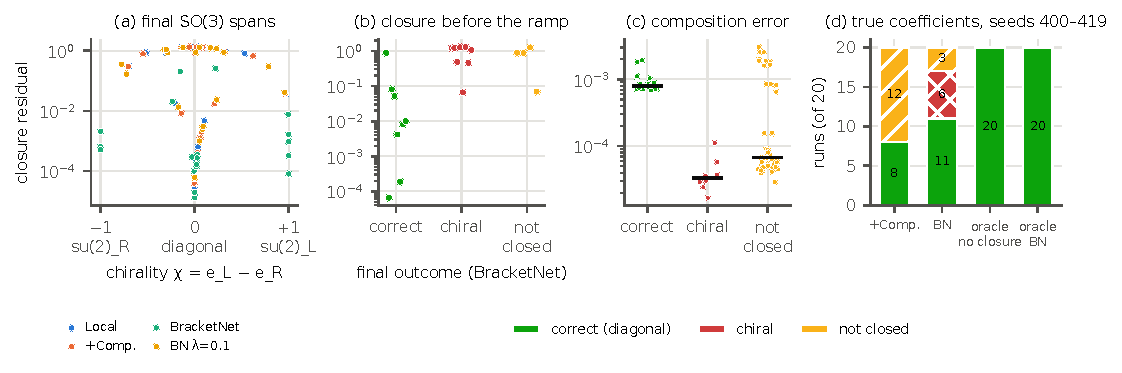
\includegraphics[width=\linewidth]{fig_mechanism.pdf}
\caption{(a) Final SO(3) span chirality $\chi$ vs.\ closure residual for every fresh-seed run: closed runs sit at
$\chi\in\{-1,0,1\}$, the classes of Prop.~\ref{prop:classify}. (b) Closure of the BracketNet span when the closure
penalty switches on, by final outcome (post hoc). (c) Composition error by outcome class, all SO(3) runs.
(d) Outcomes with endpoint-inferred vs.\ true (oracle) action coefficients, seeds 400--419.}\label{fig:mech}
\end{figure}

\subsection{A rendered-image benchmark}\label{sec:render}
To test a harder observation process, we rendered the SO(3) state as $20{\times}20$ images: the 3-D position of a
Gaussian blob sets its image position and size, and the invariant coordinate sets its brightness ($p=400$). The
frozen protocol was applied unchanged on 20 new seeds (300--319), with predictions registered in advance.
\begin{itemize}
\item \emph{No baseline run closes} (Local \REfourLocalNonclosed/20, \textsc{+Comp.} \REfourCompNonclosed/20 non-closed).
BracketNet lowers closure on \REfourClosurebnvscompWins{} seeds (\REfourBracketnetClosure{} vs.\ \REfourCompClosure,
one-sided $p=\REfourClosurebnvscompP$).
\item \emph{Every closed BracketNet run is chiral} (\REfourBracketnetChiral/20; none diagonal). This is read off the
chirality invariant, which needs no latent alignment.
\item \emph{Ground-truth recovery cannot be assessed by our alignment metric here.} The learned latents are far from
an isometry of the true state (CKA with it \REfourBracketnetCkatruth, Procrustes residual \REfourBracketnetProcrustestruth).
\item \emph{There is a small transport cost}: 10-step error rises by $\REfourMseonezerobnvscompMeandiff$
($[\REfourMseonezerobnvscompCilo,\REfourMseonezerobnvscompCihi]$).
\end{itemize}
Under rendering, closure regularization therefore produced closed algebras only of the wrong class. The benchmark is
still synthetic and does not test natural images.

\section{Representation alignment: agreement in embeddings vs.\ agreement in transformations}\label{sec:align}
Models trained from different seeds can be compared at five levels: embedding geometry, transformation algebra,
group representation, inferred action, and ground truth. We compare each pair of models on a shared probe set:
\begin{itemize}
\item \emph{alignment}: the orthogonal Procrustes map $R$ from $E_a(x)$ to $E_b(x)$, fitted on probe set A;
\item \emph{embedding agreement}: linear CKA;
\item \emph{algebra agreement}: the cross-seed algebra distance between $\spn(RA^{(a)}R^\top)$ and $\spn(A^{(b)})$;
\item \emph{transfer}: on a held-out probe set B, apply the action inferred by $a$ in $b$'s space,
$\hat x_{t+1}=D_b(R\rho_aR^\top E_b(x_t))$. The \emph{transfer gap} is $0$ when this is as good as $b$'s own action
and $1$ when it is no better than the identity.
\end{itemize}
Independent units are \NNpairs{} disjoint seed pairs, the same for every method.

\begin{table}[t]
\centering\scriptsize
\setlength{\tabcolsep}{3.5pt}
\caption{Cross-seed alignment on \NNpairs{} disjoint pairs (mean$\pm$s.d.). Algebra distance chance: $0.80$
($T^2$), $0.50$ (SO(3)). Transfer gap: 0 = native, 1 = identity. Projected: transferred actions re-expressed in
$b$'s generators.}
\label{tab:align}
\begin{tabular}{llccccc}
\toprule
Group & Method & CKA & Algebra dist. & Action disagr. & Transfer gap & Projected gap\\
\midrule
\tabinput{../../results/final/tables/alignment.tex}
\bottomrule
\end{tabular}
\end{table}

\paragraph{Algebras agree more, through a few discrete classes.}
For SO(3), the cross-seed algebra distance falls from \NHthreeSOthreeMeanb{} to \NHthreeSOthreeMeana{} (lower in
\NHthreeSOthreeWins{} pairs, Holm $p=\NHthreeSOthreeHolmp$). For $T^2$ it does not change significantly.

The SO(3) pairs separate by class:
\begin{itemize}
\item both models correct: distance $0$ (\NPtSOthreeBNBothcorrect{} pair);
\item both in the same \emph{wrong} chiral class: distance $0$ (\NPtSOthreeBNBothsameincorrecttype{} pair);
\item correct vs.\ chiral: distance $\approx\frac12$, as fixed by Prop.~\ref{prop:classify} (\NPtSOthreeBNCloseddifferenttypes{} pairs);
\item at least one model non-closed: \NPtSOthreeBNInvolvesnonclosedorcollapsed{} pairs.
\end{itemize}
All \NPtSOthreeCompInvolvesnonclosedorcollapsed{} \textsc{+Comp.} pairs involve a non-closed model and spread over
$[0,1]$. Closure thus replaces continuous disagreement with disagreement between a few closed classes, so
cross-model agreement does not certify correctness (Cor.~\ref{cor:agree}).

\paragraph{Transfer tracks structural \emph{agreement}, not correctness.}
Over all 190 pairs of each method (pooled, descriptive):
\begin{itemize}
\item SO(3) pairs of two correct models transfer almost perfectly: median gap \REfiveSOthreeBothcorrectGap{},
\REfiveSOthreeBothcorrectFail\% failures (gap $>0.5$), over \REfiveSOthreeBothcorrectN{} pairs.
\item Pairs of two models in the same wrong class also transfer: median gap \REfiveSOthreeBothsameincorrectGap{},
\REfiveSOthreeBothsameincorrectFail\% failures. Aligning them through the ground truth instead of to each other
breaks transfer (median gap \REfiveSOthreeBothsameincorrectOraclegap).
\item Correct-vs-chiral pairs transfer worse: median gap \REfiveSOthreeCorrectvsincorrectGap{},
\REfiveSOthreeCorrectvsincorrectFail\% failures.
\end{itemize}
What makes transformations reusable across models is that both models learned the \emph{same} algebra, whether or not
it is correct.

\paragraph{CKA vs.\ structural distance as predictors of transfer failure (pre-registered; prediction not supported).}
We pre-registered that the label-free algebra distance would predict transfer failure better than CKA. It did not.
\begin{itemize}
\item AUC for $T^2$: CKA \REfiveTtwoAuccka{} vs.\ algebra distance \REfiveTtwoAucdist.
\item AUC for SO(3): CKA \REfiveSOthreeAuccka{} vs.\ algebra distance \REfiveSOthreeAucdist; difference interval
$[\REfiveSOthreeDifflo,\REfiveSOthreeDiffhi]$ (seed-level cluster bootstrap).
\end{itemize}
Most transfer failures come from seed-level encoder failures, which CKA detects. CKA is, however, blind to
\emph{class} mismatches: SO(3) correct-vs-chiral pairs have median CKA \REfiveSOthreeCorrectvsincorrectCka{}, the same as
correct pairs (\REfiveSOthreeBothcorrectCka), yet a far larger transfer gap. Embedding similarity and algebra
agreement capture different failure modes, and a structural comparison needs both.

\section{Ablations}\label{sec:ablations}
Ablations use seeds 200--209 with same-seed references (Appendix Table~\ref{tab:ablations}).
\begin{itemize}
\item \emph{Replication.} \textsc{+Comp.}\ again has higher SO(3) closure and ground-truth distance than BracketNet
($+\NAbpSOthreeCompreferenceGtdistanceMeandiff$,
$[\NAbpSOthreeCompreferenceGtdistanceCilo,\NAbpSOthreeCompreferenceGtdistanceCihi]$).
\item \emph{Anti-collapse term.} Essential: at weight 1 the $T^2$ latent distorts (CKA with the truth
\NAbTtwoWeakanticollapseCkatruth) and correct-closed runs fall to \NAbTtwoWeakanticollapseCc.
\item \emph{No detectable effect}: the fit--close--refit schedule (constant penalty or no freeze), the Gram penalty,
and a span-only closure objective. We do not claim the schedule is necessary.
\item \emph{Misspecified $K$.} With $K{+}1$ no run is correct-closed (\NAbSOthreeKplusoneCc{} for SO(3)), as
Prop.~\ref{prop:classify}(c) requires.
\end{itemize}

\section{Limitations}\label{sec:limits}
\begin{itemize}
\item \textbf{Synthetic scope.} Both benchmarks, including the rendered one, are synthetic, low-dimensional and
compact, with known $K$ and orthogonal actions. We make no claim about natural images, physical systems or large models.
\item \textbf{No identifiability.} Wrong closed algebras are frequent for SO(3), and correct algebras still have
irreducible action ambiguity (Prop.~\ref{prop:endpoint}c). Our ground-truth comparisons use orthogonal Procrustes, so
they assume a near-isometric encoder; the $T^2$ failures are seed-level fitting failures shared by all methods.
\item \textbf{Limited baselines.} We compare controlled objective variants and an action-supervised oracle; we do not
reimplement published methods with different supervision.
\item \textbf{Statistics and protocol.} We use 20 seeds; effects outside SO(3) are small or concentrated in few
seeds. No transport improvement is established; on rendered images transport is slightly worse. The closure-weight rule needed an amendment, committed before any fresh
run. One pre-registered prediction (structure beats CKA at predicting transfer failure) was not supported.
\item \textbf{Theory is local, qualitative and self-checked.} The escape bound covers only small actions; the
classification is specific to $\so(4)$ and $\so(5)$; Prop.~\ref{prop:endpoint} concerns exact zeros at the
ground-truth embedding, gives no quantitative gap and says nothing about the optimization path. The proofs have not
been checked independently of the AI system that drafted them.
\end{itemize}

\section{Conclusion}\label{sec:conclusion}
Closure turns continuous disagreement between transformation models into a choice among a few closed subalgebras.
For SO(3) the choice is often wrong, because endpoints cannot reveal rotations about the axis through a point.
Agreement, of embeddings or of transformations, is not evidence of correctness.


\bibliographystyle{plainnat}
\bibliography{refs}

\newpage
\appendix
\section{Proofs}\label{app:proofs}
\paragraph{Invariance law.}
Under $B\mapsto BM$, $[A'_i,A'_j]=\sum_{k,l}M_{ki}M_{lj}[A_k,A_l]$, so the commutator matrix becomes
$C(M\otimes M)$, while $P_0(BM)=P_0(B)$. Hence $R\mapsto R(M\otimes M)$, and the bounds follow from
$\sigma(M\otimes M)=\{\sigma_i\sigma_j\}$. For $\varepsilon>0$,
$P_\varepsilon(BM)=BM(M^\top GM+\varepsilon I)^{-1}M^\top B^\top=B(G+\varepsilon M^{-\top}M^{-1})^{-1}B^\top$.

\paragraph{Proposition~\ref{prop:basic}.}
\emph{(a)} The commutator is bilinear and antisymmetric and satisfies Jacobi, so closure makes $\mathfrak a$ a Lie
subalgebra; the Lie subgroup theorem \citep[Ch.~5]{hall2015lie} gives the integrating subgroup. It need not be
closed: an irrational line in a torus is an example.

\emph{(b)} Write $X=\sum x_iA_i$, $Y=\sum y_jA_j$ and $r_{ij}=N[A_i,A_j]$. Then
$\|N[X,Y]\|\le\|x\|\|y\|(\sum\|r_{ij}\|^2)^{1/2}=\|x\|\|y\|K\sqrt{\Lc}$ by Cauchy--Schwarz, and
$\|X\|^2=x^\top Gx\ge\lambda_{\min}\|x\|^2$.

\emph{(c)} Dynkin's form \citep{bonfiglioli2012topics} is
$\log(e^Xe^Y)=\sum_{m\ge1}\frac{(-1)^{m-1}}{m}\sum\frac{[w]}{|w|\prod r_i!s_i!}$, summed over words
$w=X^{r_1}Y^{s_1}\cdots X^{r_m}Y^{s_m}$ with $r_i+s_i\ge1$, where $[w]$ is right-nested.
\begin{itemize}
\item By submultiplicativity, $\|[w]\|\le2^{|w|-1}r^{|w|}$.
\item Let $e_n$ bound $\|N[w]\|$ for $|w|=n$, so $e_1=0$ and $e_2\le\delta r^2$. Write $[w]=[W,Z]$ with $W$ a letter.
\item $[W,P_0Z]$ has both arguments in $\mathfrak a$, so its escape is at most $\delta r\|Z\|\le\delta2^{n-2}r^n$;
and $\|[W,NZ]\|\le2re_{n-1}$. By induction $e_n\le(n-1)2^{n-2}\delta r^n$.
\item Each word therefore contributes at most $\frac{\delta}{4}(2r)^{|w|}/\prod r_i!s_i!$. The full sum is
$\sum_m\frac1m(e^{4r}-1)^m=-\ln(2-e^{4r})$ for $r<\ln2/4$.
\item The length-1 words lie in $\mathfrak a$ and account for $4r$; subtracting them gives the bound.
\item The length-2 words sum to $\frac12[X,Y]$, whose escape is at most $\frac12\delta r^2$; replacing their crude
contribution $4\delta r^2$ gives $\frac12\delta r^2+O(\delta r^3)$.
\item The series converges absolutely on this ball, and the principal logarithm is analytic there
($\|e^Xe^Y-I\|<1$). Both sides agree near $0$, hence on the whole connected ball.
\end{itemize}

\emph{(d)} With $d_t=\hat z_t-z_t$: $d_{t+1}=R_td_t-e_t$ and $\|R_td_t\|=\|d_t\|$.
$\square$

\paragraph{Proposition~\ref{prop:classify}.}
Subalgebras of $\so(d)$ carry the ad-invariant negative-definite form $\operatorname{tr}(XY)$, hence are compact and
reductive.

\emph{(a)} A 2-dimensional reductive algebra is abelian. It is maximal abelian because
$\operatorname{rank}\so(5)=2$, and maximal abelian subalgebras of a compact Lie algebra are conjugate
\citep{adams1969lectures}.

\emph{(b)} A 3-dimensional reductive $\mathfrak h$ is its center plus a semisimple part of dimension $0$ or $3$.
It cannot be abelian (the rank is 2), so $\mathfrak h\cong\su(2)$. Its projections onto the ideals $\su(2)_{L},\su(2)_{R}$ are zero or injective, because
$\mathfrak h$ is simple.
\begin{itemize}
\item If one projection is zero, $\mathfrak h$ is a factor. The factors are ideals, hence invariant under all of
$SO(4)$, and a reflection exchanges them.
\item Otherwise $\mathfrak h$ is the graph of an isomorphism $\su(2)_L\to\su(2)_R$. Any two such graphs differ
by an automorphism of $\su(2)$, which is inner, and $SU(2)\times SU(2)\to SO(4)$ is onto, so all such $\mathfrak h$
are $SO(4)$-conjugate. The stabilizer of $e_4$, $\so(3)$ on $\mathbb R^3\oplus\mathbb R$, is one of them (it is not
an ideal).
\item $SO(4)$ is connected, so it cannot exchange the two ideals; hence three classes under $SO(4)$ and, since a
reflection fixing $e_4$ exchanges them and preserves the diagonal, two under $O(4)$.
\end{itemize}
The Pfaffian is $SO(4)$-invariant and odd under reflections. It vanishes on rank-2 rotations and equals
$\pm\frac12$ on unit elements of $\su(2)_{L/R}$.

\emph{(c)} A 4-dimensional reductive subalgebra is $\su(2)\oplus\mathfrak u(1)$ with the $\mathfrak u(1)$ central.
The centralizer of the diagonal $\so(3)$ is trivial, because $\so(4)\cong\Lambda^2\mathbb R^4$ decomposes as
$\mathbf 3\oplus\mathbf 3$ under it, with no trivial summand; the same holds for its conjugates. So the $\su(2)$ is
a factor, which equals the derived algebra $[\mathfrak h,\mathfrak h]$. A diagonal $\so(3)\subset\mathfrak h$ would
satisfy $\so(3)=[\so(3),\so(3)]\subset[\mathfrak h,\mathfrak h]$, a factor, which is impossible.

\emph{Scope.} The classification is for exactly closed spans. Learned spans are only approximately closed; we assign
them to classes using continuous invariants (Pfaffian, chirality) and the closure-flow check, without a stability
theorem relating approximate closure to distance from a closed class. $\square$

\paragraph{Proposition~\ref{prop:endpoint}.}
Here $g\in SO(3)$ acts on $z_{1:3}$ and fixes $z_4$, so transitions preserve $\|z\|$.

\emph{(a)} Identify $\mathbb R^4$ with the quaternions $\mathbb H$. The exponential of $\su(2)_L$ is left
multiplication by unit quaternions, which acts simply transitively on each sphere $\|z\|=\rho>0$. For
$\|z\|=\|z'\|$, $u=z'z^{-1}$ is the unique unit quaternion with $L_uz=z'$.
\begin{itemize}
\item $q=\log u$ is smooth wherever $u\neq-1$, and $\exp(\log u)=u$ for every branch.
\item $u_{02}=z_2z_0^{-1}=(z_2z_1^{-1})(z_1z_0^{-1})=u_{12}u_{01}$, so composition is exact.
\item Closure is exact, the basis is orthonormal so the Gram penalty is $0$, and $\mathrm{Cov}(z)=I$ in population
(states are $\mathcal N(0,I)$ and rotations preserve that law).
\end{itemize}
The coefficient of a rotation by angle $\theta=\angle(z,z')$ has entries up to $\sqrt2\theta$; only pairs beyond the
bound $0.65$ break exactness.

\emph{(b)} Fix the sphere $S$ and suppose a continuous rule gives $R(z,z')=\rho(q(z,z'))\in SO(3)$ with
$R(z,z')z=z'$ and $R(z_0,z_2)=R(z_1,z_2)R(z_0,z_1)$ for all $z_i\in S$ with pairwise angles $<\epsilon$.
\begin{itemize}
\item The triple $(z,z,z)$ gives $R(z,z)=R(z,z)^2$, so $R(z,z)=I$.
\item For a chain $x_0,\dots,x_n$ with consecutive angles $<\epsilon/3$, let $P=R(x_{n-1},x_n)\cdots R(x_0,x_1)$.
Inserting or deleting a point inside an $\epsilon$-small triangle leaves $P$ unchanged. Two chains with the same
endpoints and pointwise angles $<\epsilon/3$ are joined by such moves (replace one point at a time; each move is a
triangle of diameter $<\epsilon$), so $P$ is unchanged. Fine subdivisions of a continuous path therefore define one
$P$, and by uniform continuity it is constant along a homotopy of paths with fixed endpoints.
\item $S\cong S^2$ is simply connected, so fixing $e\in S$, $s(z)=P(e\to z)$ is well defined, with $s(z)e=z$.
It is continuous, because $s(z')=R(z,z')s(z)$ for nearby $z'$ and $R$ is continuous with $R(z,z)=I$.
\item For a unit $f\perp e$ (in the $\mathbb R^3$ part), $z\mapsto s(z)f$ is orthogonal to $s(z)e=z$: a
nowhere-vanishing tangent field on $S^2$, contradicting the hairy-ball theorem.
\end{itemize}
The rule takes values in the true (diagonal) group; the argument uses no property of $q$ beyond continuity.

\emph{(c)} For fixed endpoints $(z,z')$ with $z_{1:3}\neq0$, the set $\{g:gz=z'\}$ is a coset of the circle
stabilizing $z$. The states have a density and $\exp$ pushes the Gaussian coefficients to a law with a density on
$SO(3)$, so the conditional law of $g$ on that circle has a density for almost every $(z,z')$. Hence
$\mathbb E\|\hat g-g\|^2\ge\mathbb E\,\operatorname{tr}\operatorname{Cov}(g\mid z,z')>0$ for every endpoint
estimator $\hat g$. $\square$

\paragraph{Remark (what Prop.~\ref{prop:endpoint}b does not show).}
\begin{itemize}
\item \emph{Continuity is essential.} $S$ minus one point is contractible, so $SO(3)\to S^2$ has a continuous
section $s$ there. Ignoring the coefficient bound, $R(z,z')=s(z')s(z)^{-1}$ is a measurable rule that is exact on
every triple avoiding that point, i.e.\ off a null set.
\item \emph{A gap for any fixed Lipschitz class.} Let $J_\epsilon(q)$ be the expected transport and composition loss
on data triples with pairwise angles $<\epsilon$, small enough that the chiral rule is within the bound
($J_\epsilon=0$ for it). For every $L$, the infimum of $J_\epsilon$ over $L$-Lipschitz rules with bounded
coefficients is positive for the true algebra. Otherwise, by Arzel\`a--Ascoli a subsequence converges locally
uniformly to such a rule with $J_\epsilon=0$, by dominated convergence (bounded integrand). The integrand is
continuous and the support contains every such triple on every orbit sphere, so the rule is exact there, which
contradicts (b).
\item \emph{No quantitative statement.} We do not bound this gap, and it may vanish as $L\to\infty$. Nor do we
compare the full training objective, which includes large steps and clipping, between the two algebras.
\end{itemize}

\paragraph{Corollary~\ref{cor:agree}.}
This is Prop.~\ref{prop:endpoint}(a) applied to both models, together with Prop.~\ref{prop:classify}(b) and the
distance $\frac12$ between the diagonal and a chiral span. $\square$


\section{Protocol details}\label{app:protocol}
\paragraph{Architecture and optimization.}
$E,D,q$ are two-hidden-layer SiLU MLPs of width 64. The latent dimension is $d$, generators are initialized as
$W\sim\mathcal N(0,1/d)$, and coefficients are $0.65\tanh(\cdot)$. Training uses AdamW (lr $2\times10^{-3}$, weight
decay $10^{-5}$), batch 160, gradient clipping at 5, $\varepsilon=10^{-6}$, Gram weight 1 and anti-collapse weight 16.
The anti-collapse weight was chosen in a preliminary round on seeds 5--6 by a method-agnostic criterion. The final
iterate is evaluated, with no early stopping. All runs are CPU-only and bit-identical on repeat.

\paragraph{Order of operations.}
\begin{enumerate}
\item Selection rules committed.
\item Development grid (280 runs).
\item Rules applied by script.
\item Fresh seeds 100--119 and ablation seeds 200--209, each run once.
\item Review predictions committed.
\item Trace, oracle and rendered runs.
\end{enumerate}
No setting was changed after any fresh-seed result was seen.

\paragraph{Rendered benchmark.}
The image has $20\times20$ pixels on $[-3.2,3.2]^2$. The blob centre is $(z_1,z_2)$, its width is
$0.45\,e^{0.3z_3}$ and its amplitude is $1+0.5\tanh z_4$. Positions are scaled by $0.7$ so that blobs stay in view.
Centre, width and amplitude determine $z$, so the map is injective.

\paragraph{Oracle intervention.}
The transport terms use the true coefficients of each training edge. The composition term is dropped, because
$a_{02}$ is a product rather than a single coefficient. $q$ is trained only by regression to the true coefficients,
for evaluation.

\section{Statistical audit}\label{app:stats}
The six primary tests were recomputed from the raw run files by an independent implementation, and all matched. The
$t$-interval can disagree with the primary sign-flip test when differences are skewed, so we also report the interval
obtained by inverting the two-sided exact sign-flip test, which matches the primary procedure, and a percentile
bootstrap interval.

\begin{table}[ht]
\centering\scriptsize
\setlength{\tabcolsep}{2.4pt}
\caption{Paired differences (BracketNet $-$ +Comp.). Intervals: $t$; sign-flip-inverted; bootstrap.}
\begin{tabular}{llcccccc}
\toprule
Test & Group & $n$ & median diff. & skew & $t$ 95\% & inverted sign-flip 95\% & bootstrap 95\%\\
\midrule
\tabinput{../../results/review/tables/stats_audit.tex}
\bottomrule
\end{tabular}
\end{table}

\paragraph{Threshold sensitivity (robustness check, not pre-registered).}
SO(3) fresh-seed counts (correct / chiral / other closed / non-closed) under alternative thresholds, as a fraction of
the random-span closure level and of the chance distance:
\begin{center}\scriptsize
\begin{tabular}{cccc}
\toprule
closed & correct & +Comp. & BracketNet\\
\midrule
\tabinput{../../results/review/tables/threshold_sensitivity.tex}
\bottomrule
\end{tabular}
\end{center}
The qualitative conclusions (no chiral solutions without closure; several with it; more correct-closed runs with
closure) hold at every setting.

\section{Comparison of settings}\label{app:novelty}
\begin{table}[ht]
\centering\scriptsize
\setlength{\tabcolsep}{3pt}
\begin{tabular}{p{2.9cm}p{2.6cm}p{2.3cm}p{2.0cm}p{1.9cm}}
\toprule
Work & Supervision & Learned structure & Closure & Cross-model structure\\
\midrule
Rao \& Ruderman; Sohl-Dickstein et al. & transformed pairs & linear generators & not enforced & no\\
Cohen \& Welling 2014 & pairs, commutative group & irreps of a torus & abelian by design & no\\
LieGAN / LaLiGAN & distributional invariance & generators (latent) & not penalized & no\\
Homomorphism AE & transitions + action labels & homomorphism into matrix group & via composition & no\\
CKA / shape metrics & trained networks & --- & --- & embeddings only\\
This work & transitions, no labels & generators + endpoint actions & closure penalty & algebras, transfer\\
\bottomrule
\end{tabular}
\end{table}
These summaries describe each setting at the level needed to judge overlap; see the cited papers for details.

\section{Additional results}\label{app:results}
\begin{table}[ht]
\centering\scriptsize
\setlength{\tabcolsep}{3pt}
\caption{Structural breakdown of fresh-seed runs (counts out of 20). Incorrect-closed runs are shown with the chiral
count in parentheses. ``Bad action'' counts correct-closed runs whose action disagreement with the truth exceeds 0.5.
PR: participation ratio.}
\label{tab:structure}
\begin{tabular}{llccccccc}
\toprule
Group & Method & Correct & Incorrect (chiral) & Non-closed & Collapsed & Bad action & Action disagr. & PR\\
\midrule
\tabinput{../../results/final/tables/structure.tex}
\bottomrule
\end{tabular}
\end{table}

\begin{table}[ht]
\centering\scriptsize
\setlength{\tabcolsep}{3pt}
\caption{Ablations on seeds 200--209 (mean$\pm$s.d.). Coverage is the fraction of the true span contained in the
learned span. Categories: correct / incorrect / non-closed / collapsed. With misspecified $K$, ``correct'' is
impossible by definition.}
\label{tab:ablations}
\begin{tabular}{llccccc}
\toprule
Group & Variant & 10-step MSE & Closure & GT dist. & Coverage & Categories\\
\midrule
\tabinput{../../results/final/tables/ablations.tex}
\bottomrule
\end{tabular}
\end{table}

\begin{table}[ht]
\centering\scriptsize
\caption{Development grid (seeds 5--9; selection only; means over 5 seeds). For each method: 10-step MSE,
closure, correct-closed count.}
\label{tab:devbudget}
\begin{tabular}{llccccccccc}
\toprule
& & \multicolumn{3}{c}{Local} & \multicolumn{3}{c}{+Comp.} & \multicolumn{3}{c}{BracketNet}\\
Group & Updates & MSE & closure & CC & MSE & closure & CC & MSE & closure & CC\\
\midrule
\tabinput{../../results/final/tables/dev_budget.tex}
\bottomrule
\end{tabular}
\end{table}

\begin{figure}[ht]\centering
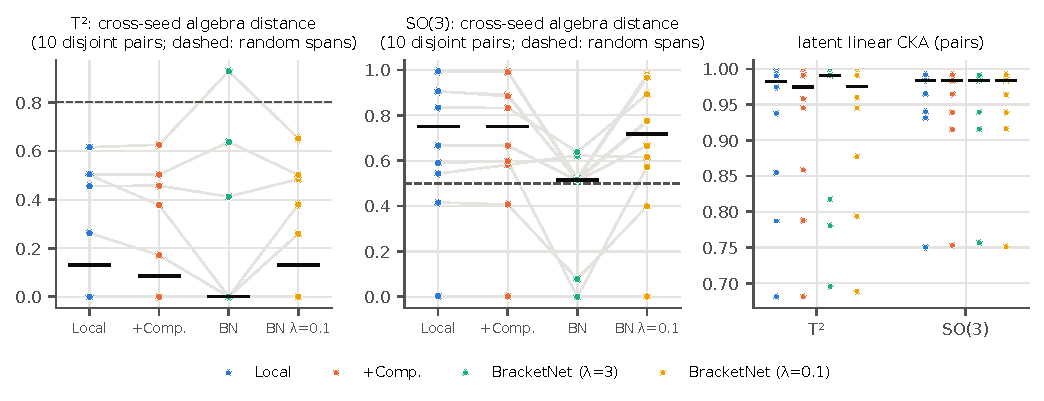
\includegraphics[width=\linewidth]{fig_alignment.pdf}
\caption{Cross-seed algebra distance on 10 disjoint pairs (grey lines join the same pair across methods; BN =
BracketNet) and latent CKA.}\label{fig:align}
\end{figure}

\begin{figure}[ht]\centering
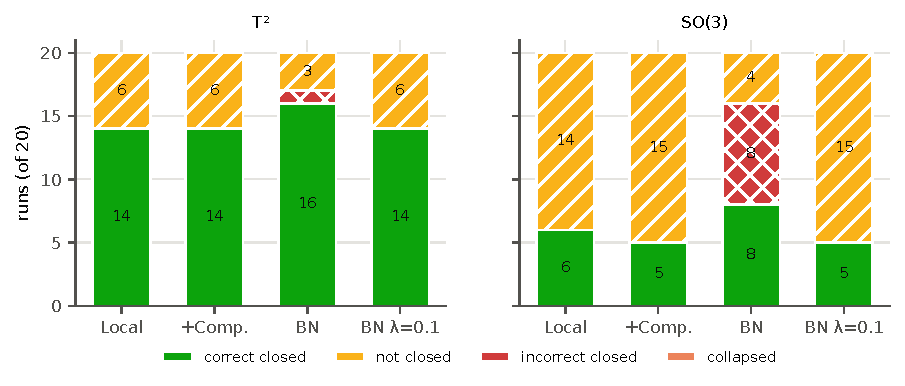
\includegraphics[width=\linewidth]{fig_categories.pdf}
\caption{Structural category of each fresh-seed run (BN = BracketNet).}\label{fig:cat}
\end{figure}

\begin{figure}[ht]\centering
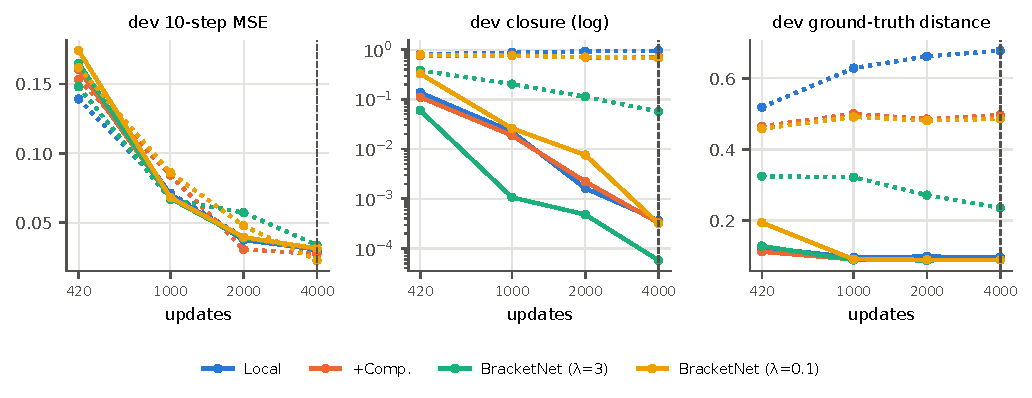
\includegraphics[width=\linewidth]{fig_dev_budget.pdf}
\caption{Development-seed budget sweep (solid: $T^2$; dotted: SO(3)); the vertical line marks the selected budget.}
\end{figure}

\begin{figure}[ht]\centering
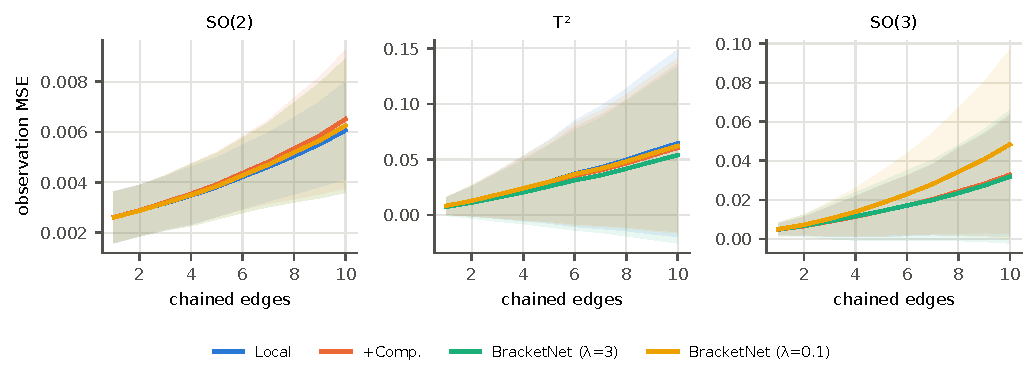
\includegraphics[width=\linewidth]{fig_transport.pdf}
\caption{Chained transport error (mean $\pm$ s.d., 20 fresh seeds).}
\end{figure}

\section{Reproducibility}
The anonymized supplement contains the data generator, models, training and analysis code, the selection rules and
review predictions, per-run result files for every run, the fresh-seed checkpoints, figure scripts and unit tests.
Every number in the text is generated as a \LaTeX{} macro from the raw files.


\section{Use of AI assistance}
Code, experiments, analyses and drafts of this manuscript were developed with substantial assistance from an AI
coding assistant. The authors are responsible for all content and have checked the claims, proofs and results.

\end{document}
